\chapter{Sample Data}
\label{chp:data-summary-tables}
This chapter contains full summary tables for the first hand data collected (Section \ref{sec:summary-tables}) and plots of sample data (Section \ref{sec:example-data-plots}).

\clearpage
\section{Summary Tables of Collected Data}
\label{sec:summary-tables}
Table \ref{tab:complete-demographic-data} contains the demographic data for all test subjects. Table \ref{tab:methods-phase-1-data-summary} contains a summary of the data collected during the first phase of data collection. Table \ref{tab:methods-phase-2-data-summary} show a summary of the data collected during the second phase. Table \ref{tab:methods-phase-3-data-summary} contains a summary of the first hand data collected during for one left trans-tibial individual.

\begin{table}[!htb]
    \centering
    \caption{Table of demographic data for study subjects}
    \label{tab:complete-demographic-data}
    \begin{tabularx}{\textwidth}{cYYYY}
    \noalign{\hrule height 1.5pt}
        \textbf{Subject ID} & \textbf{Age} & \textbf{Gender} & \textbf{Height [cm]} & \textbf{Weight [Kg]} \\
        \hline
        01 & 27 & Male & 185 & 75 \\
        02 & 24 & Male & 180 & 77 \\ 
        03 & 25 & Male & 180 & 80 \\ 
        04 & 23 & Male & 180 & 72 \\ 
        05 & 24 & Male & 178 & 82 \\ 
        06 & 23 & Male & 170 & 68 \\ 
        07 & 24 & Male & 172 & 68 \\ 
        08 & 24 & Male & 165 & 80 \\ 
        09 & 26 & Female & 173 & 65 \\
        10 & 23 & Male & 180 & 75 \\ 
        11 & 26 & Male & 185 & 75 \\
        12 & 26 & Female & 170 & 68 \\
        13 & 45 & Male & 175 & 80 \\
        14 & 26 & Male & 182 & 85 \\
        15 & 25 & Male & 180 & 75 \\
        16 & 26 & Male & 187 & 80 \\
        17 & 25 & Female & 161 & 60 \\
        18 & 23 & Female & 163 & 63 \\
        19 & 24 & Female & 165 & 65 \\
        20 & 26 & Male & 186 & 90 \\
        21 & 63 & Female & 165 & 75 \\
        22 & 25 & Male & 185 & 70 \\
        A1 & 56 & Male & 178 & 70 \\
        \noalign{\hrule height 1.5pt}
    \end{tabularx}
\end{table}

% General data
\begin{table}[p]
    \centering
    \caption[Data samples of non-amputee data collected during the first phase of collection]{Summary of non-amputee data collected during the first phase of collection. (\acrfull{ra}, \acrfull{rd}, \acrfull{sa}, \acrfull{sd})}
    \label{tab:methods-phase-1-data-summary}
    %W---Walking, RA---Ramp Ascent, RD---Ramp Descent, SA---Stair Ascent, SD---Stair Descent, S---Stopped
    \begin{tabularx}{\textwidth}{cYYYYYY}
      \noalign{\hrule height 1.5pt}
      \textbf{Subject ID} & \textbf{WALK} & \textbf{\glsentryshort{ra}} & \textbf{\glsentryshort{rd}} & \textbf{\glsentryshort{sa}} & \textbf{\glsentryshort{sd}} & \textbf{STOP} \\
      \hline
        01 & 34618 & 0 & 0 & 5349 & 5025 & 1281 \\
        02 & 13564 & 0 & 0 & 4614 & 4447 & 1020 \\
        03 & 5005 & 0 & 0 & 3633 & 2568 & 1587 \\
        04 & 32336 & 0 & 0 & 6045 & 5482 & 0 \\
        05 & 32525 & 0 & 0 & 6621 & 5767 & 0 \\
        06 & 37895 & 0 & 0 & 8424 & 5636 & 0 \\
        07 & 21843 & 0 & 0 & 14074 & 10873 & 0 \\
        08 & 38590 & 0 & 0 & 11036 & 17801 & 0 \\
        09 & 40384 & 0 & 0 & 10826 & 7953 & 0 \\
        10 & 37353 & 0 & 0 & 10812 & 8084 & 0 \\
        11 & 8341 & 0 & 0 & 1614 & 1566 & 0 \\
        12 & 9038 & 0 & 0 & 6273 & 4926 & 0 \\
        13 & 252022 & 48821 & 53735 & 18778 & 16220 & 16887 \\
        14 & 302440 & 18531 & 18305 & 10936 & 9581 & 73781 \\
        15 & 12249 & 0 & 0 & 1452 & 1929 & 3498 \\
        16 & 23729 & 0 & 0 & 5332 & 2578 & 1651 \\
        17 & 113222 & 2702 & 3754 & 3190 & 3949 & 19127 \\
        18 & 37352 & 0 & 0 & 3747 & 2565 & 1133 \\
        19 & 4990 & 0 & 0 & 1240 & 1245 & 0 \\
        20 & 3487 & 0 & 0 & 2383 & 3054 & 0 \\
        21 & 4806 & 0 & 0 & 2551 & 190 & 206 \\
        22 & 9033 & 3274 & 3630 & 982 & 938 & 856 \\
        \hline
        \textbf{Total} & 1075111 & 73328 & 79426 & 139915 & 122378 & 121027 \\
        \noalign{\hrule height 1.5pt}
    \end{tabularx}
\end{table}

% Personalisation data
\begin{table}[p]
    \centering
    \caption[Data samples of non-amputee data collected during the second phase of collection]{Data samples of non-amputee data collected during the second phase of collection. (\acrfull{ra}, \acrfull{rd}, \acrfull{sa}, \acrfull{sd})}
    \begin{tabularx}{\textwidth}{cYYYYYY}
      \noalign{\hrule height 1.5pt}
      \textbf{Subject ID} & \textbf{WALK} & \textbf{\glsentryshort{ra}} & \textbf{\glsentryshort{rd}} & \textbf{\glsentryshort{sa}} & \textbf{\glsentryshort{sd}} & \textbf{STOP} \\
      \hline
      01 & 462446 & 141268 & 139786 &59685 & 44024 & 62397 \\
      03 & 291213 & 77508 & 59157 & 48695 & 50210 & 157867 \\
      09 & 368090 & 115299 & 82980 & 49530 & 51698 & 60605 \\
      \hline
      \textbf{Total} & 2100308 & 404127 & 364574 & 277250 & 252494 & 363669 \\
      \noalign{\hrule height 1.5pt}
    \end{tabularx}
    \label{tab:methods-phase-2-data-summary}
\end{table}

% Amputee data
\begin{table}[p]
    \centering
    \caption[Data samples of first hand amputee data collected during the third phase of collection]{Data samples of first hand amputee data collected during the third phase of collection. (\acrfull{ra}, \acrfull{rd}, \acrfull{sa}, \acrfull{sd})}
    \begin{tabularx}{\textwidth}{cYYYYYY}
      \noalign{\hrule height 1.5pt}
      \textbf{Subject ID} & \textbf{WALK} & \textbf{\glsentryshort{ra}} & \textbf{\glsentryshort{rd}} & \textbf{\glsentryshort{sa}} & \textbf{\glsentryshort{sd}} & \textbf{STOP} \\
      \hline
      A1 & 38114 & 6159 & 7194 & 2872 & 2450 & 11763 \\
      \noalign{\hrule height 1.5pt}
    \end{tabularx}
    \label{tab:methods-phase-3-data-summary}
\end{table}

\clearpage
\section{Example Sensor Data}
\label{sec:example-data-plots}
Within this section example plots of the recorded sensor data are provided for reference. The accelerometer and gyroscope data for each of the five sensor locations are included. Each Figure shows example data for each of the six activities labelled.

Figures \ref{fig:example-left-ankle-accel-sensor-data} and \ref{fig:example-left-ankle-gyro-sensor-data} show example data for the left ankle accelerometer and gyroscope respectively. Figures \ref{fig:example-right-ankle-accel-sensor-data} and \ref{fig:example-right-ankle-gyro-sensor-data} the right ankle. Figures \ref{fig:example-left-ankle-accel-sensor-data} and \ref{fig:example-left-hip-gyro-sensor-data} show the left hip and Figures \ref{fig:example-right-hip-accel-sensor-data} and \ref{fig:example-right-hip-gyro-sensor-data} the right hip. Figures \ref{fig:example-chest-accel-sensor-data} and \ref{fig:example-chest-gyro-sensor-data} contain example plots for the chest accelerometer and gyroscope.

%---------------------- LEFT ANKLE ------------------------
% Left Ankle - Accelerometer data
\begin{figure}[p]
\centering
    \begin{subfigure}[b]{0.49\textwidth}
         \centering
         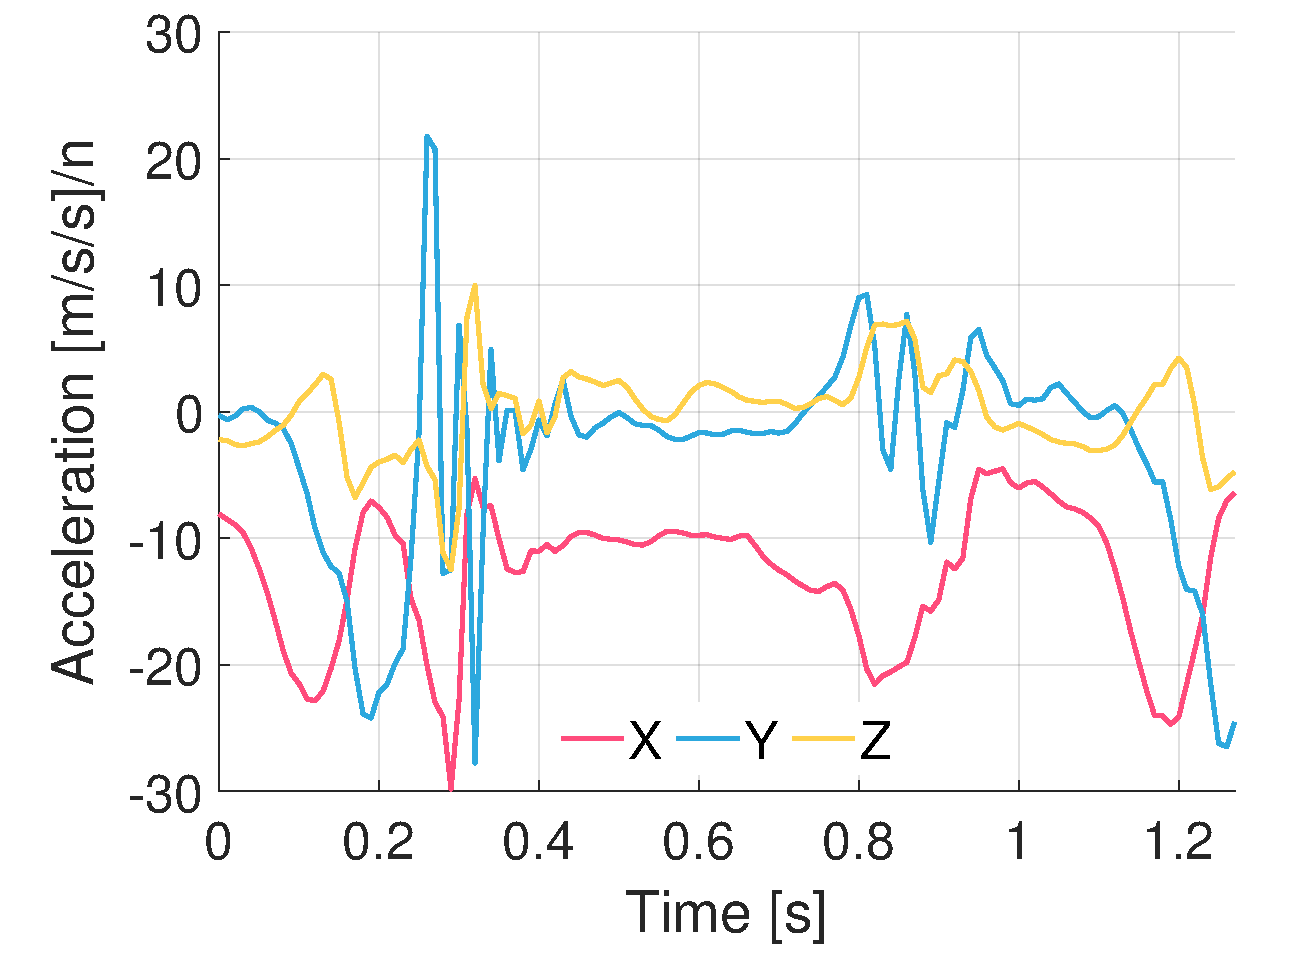
\includegraphics[width=\textwidth]{content/3-Methods/example-data/ch3_example_data_subject_01_l_ankle_accel_activity_walking.pdf}
         \caption{Walking}
    \end{subfigure}
    \begin{subfigure}[b]{0.49\textwidth}
         \centering
         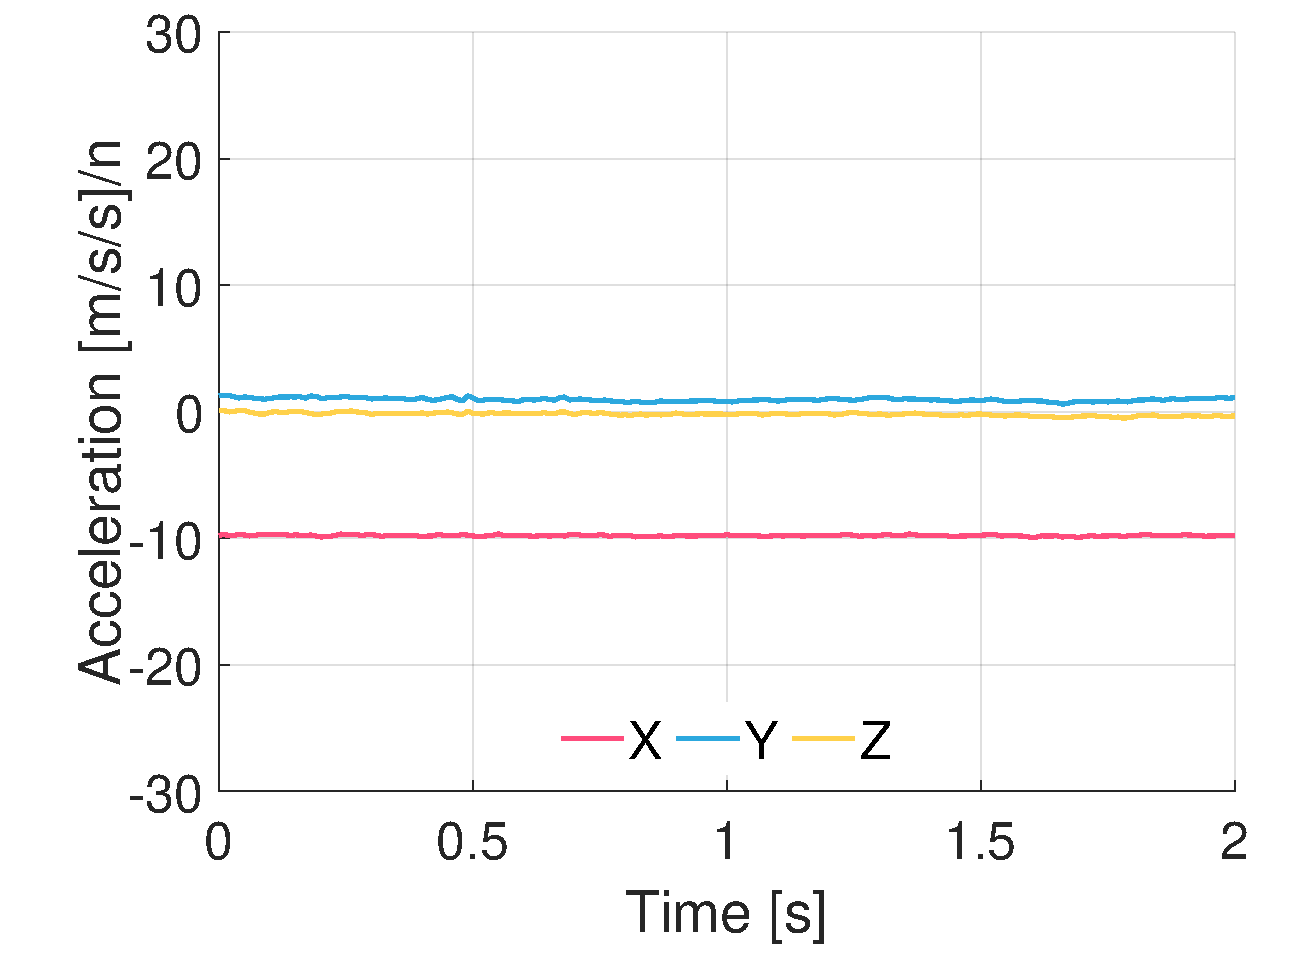
\includegraphics[width=\textwidth]{content/3-Methods/example-data/ch3_example_data_subject_01_l_ankle_accel_activity_stop.pdf}
         \caption{Stopped}
    \end{subfigure}
    
    \begin{subfigure}[b]{0.49\textwidth}
         \centering
         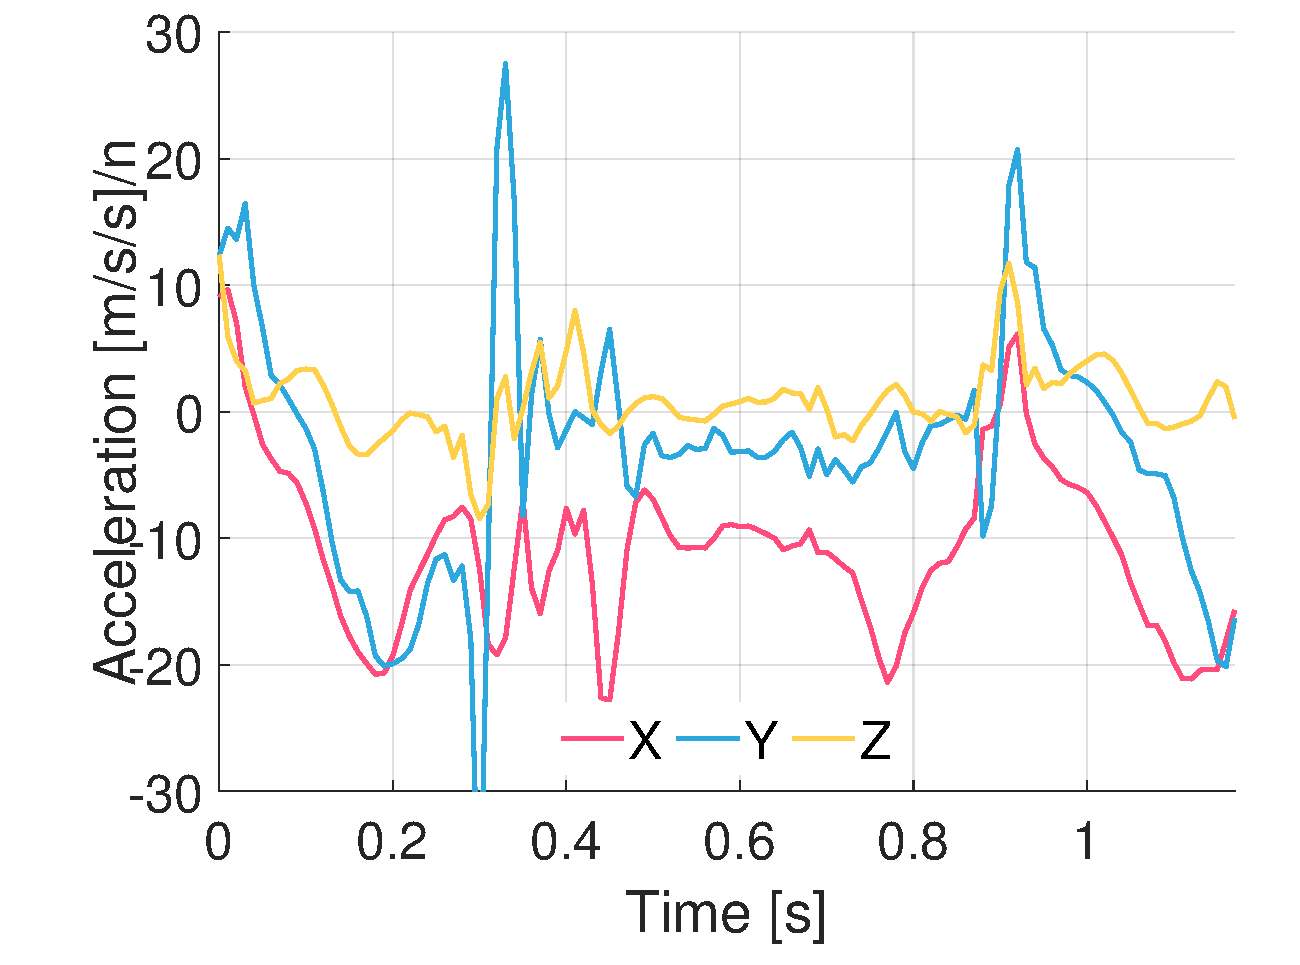
\includegraphics[width=\textwidth]{content/3-Methods/example-data/ch3_example_data_subject_01_l_ankle_accel_activity_stair_down.pdf}
         \caption{Stair Ascent}
    \end{subfigure}
    \begin{subfigure}[b]{0.49\textwidth}
         \centering
         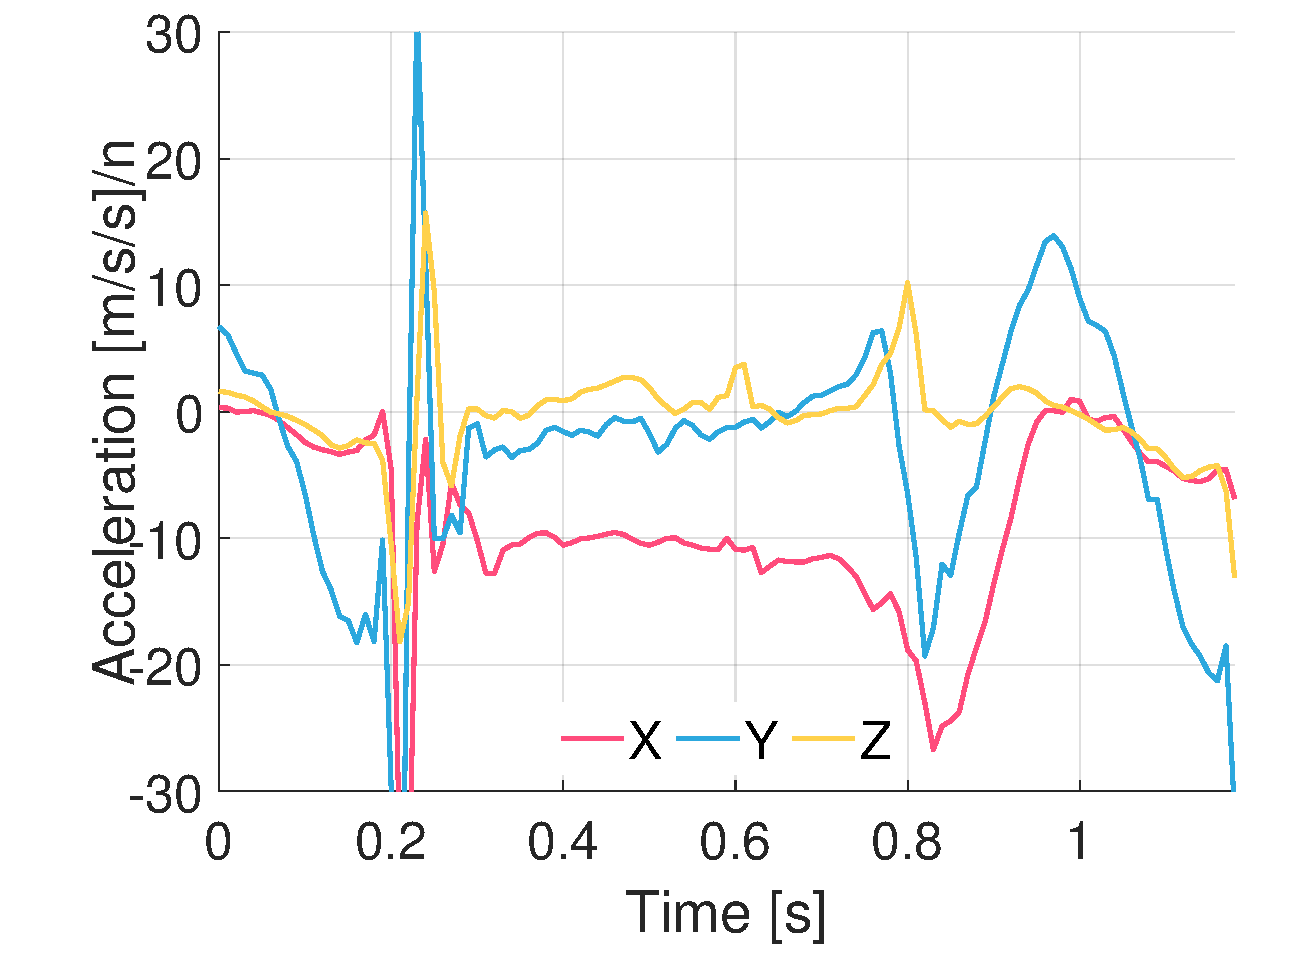
\includegraphics[width=\textwidth]{content/3-Methods/example-data/ch3_example_data_subject_01_l_ankle_accel_activity_stair_up.pdf}
         \caption{Stair Descent}
    \end{subfigure}
    
    \begin{subfigure}[b]{0.49\textwidth}
         \centering
         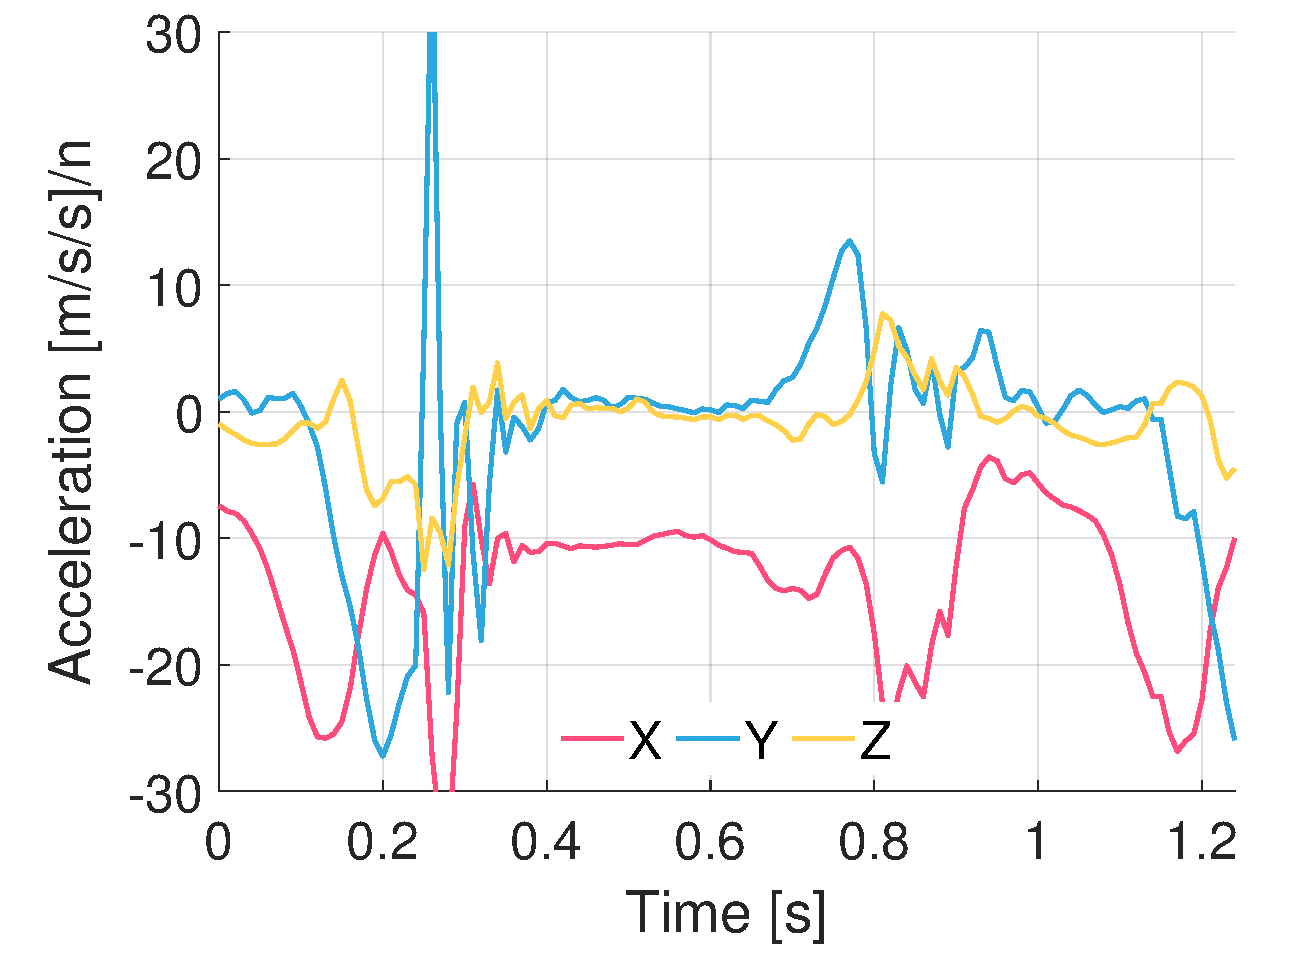
\includegraphics[width=\textwidth]{content/3-Methods/example-data/ch3_example_data_subject_01_l_ankle_accel_activity_ramp_up.pdf}
         \caption{Ramp Ascent}
    \end{subfigure}
    \begin{subfigure}[b]{0.49\textwidth}
         \centering
         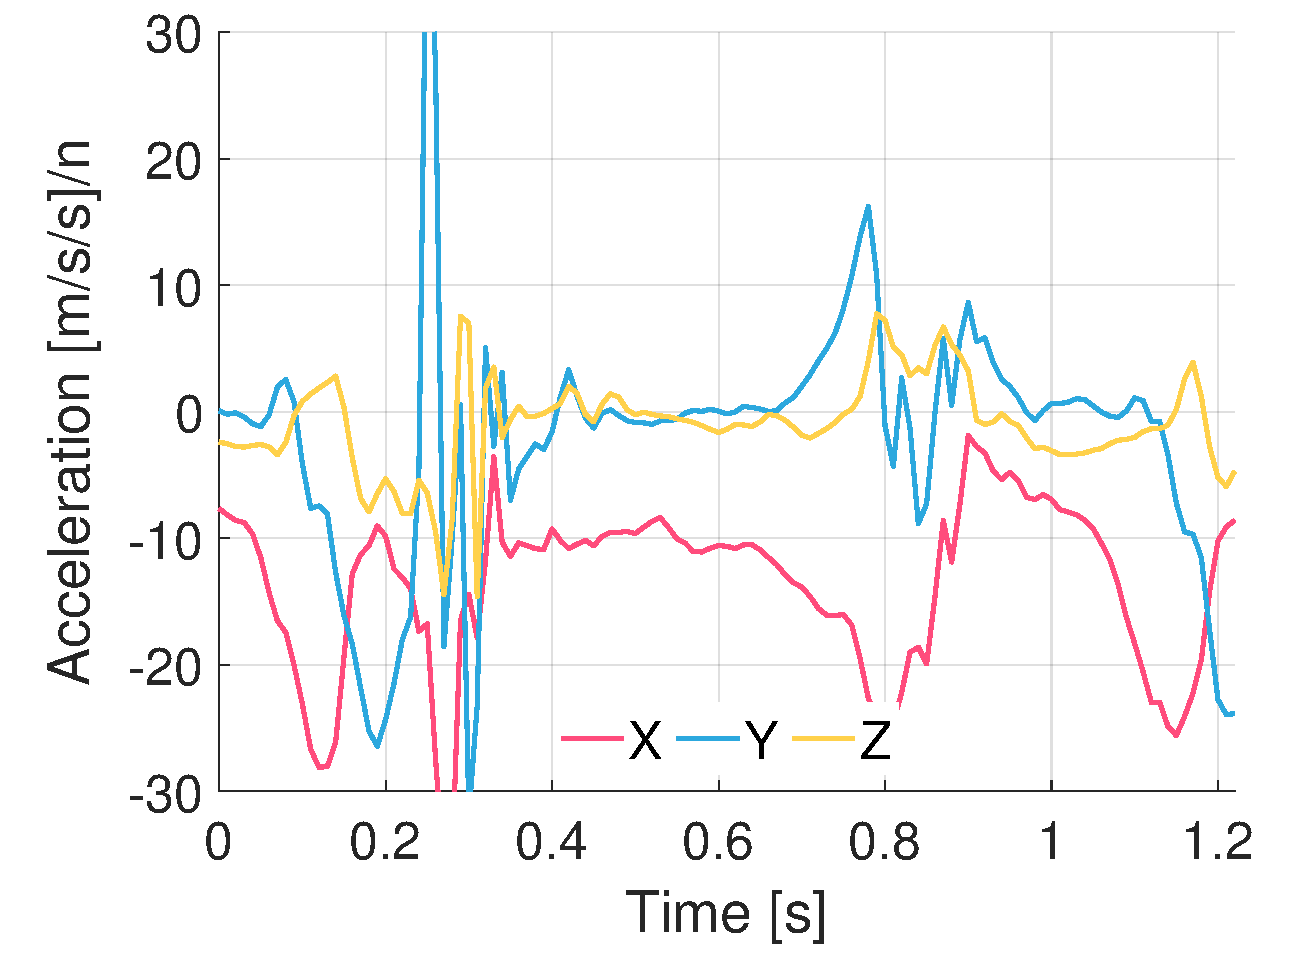
\includegraphics[width=\textwidth]{content/3-Methods/example-data/ch3_example_data_subject_01_l_ankle_accel_activity_ramp_down.pdf}
         \caption{Ramp Descent}
    \end{subfigure}
    \caption[Example left ankle accelerometer data]{Example data for the left ankle accelerometer. The $x$ represent recording time in seconds. The y axis show the measured acceleration in m/s/s. The red lines represents the $x$ axis of the sensor, the blue solid lines the $y$ axis and the yellow lines the $z$ axis.}
    \label{fig:example-left-ankle-accel-sensor-data}
\end{figure}

% Left ankle gyro
\begin{figure}[p]
\centering
    \begin{subfigure}[b]{0.49\textwidth}
         \centering
         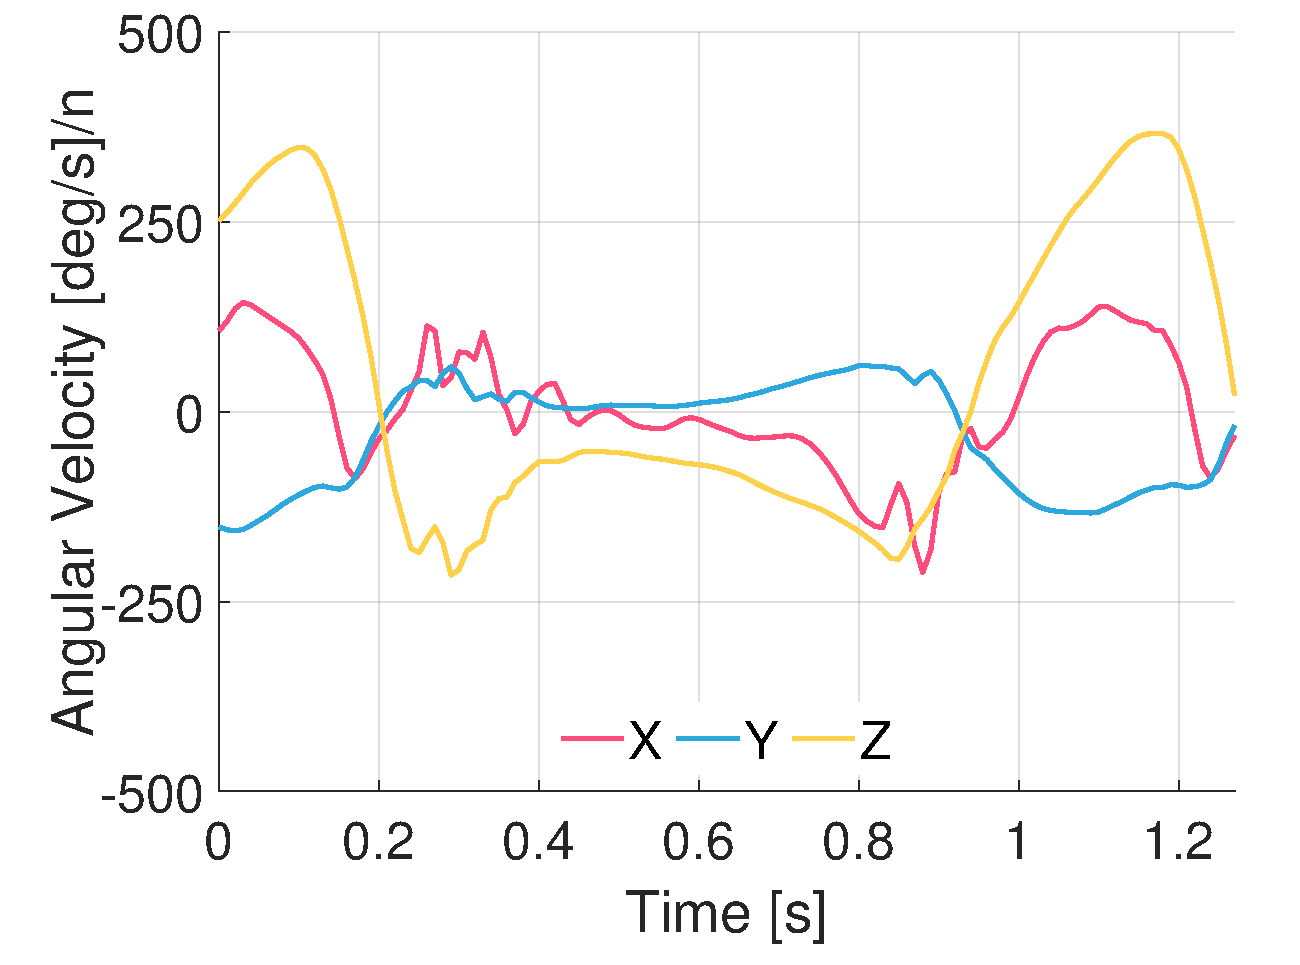
\includegraphics[width=\textwidth]{content/3-Methods/example-data/ch3_example_data_subject_01_l_ankle_gyro_activity_walking.pdf}
         \caption{Walking}
    \end{subfigure}
    \begin{subfigure}[b]{0.49\textwidth}
         \centering
         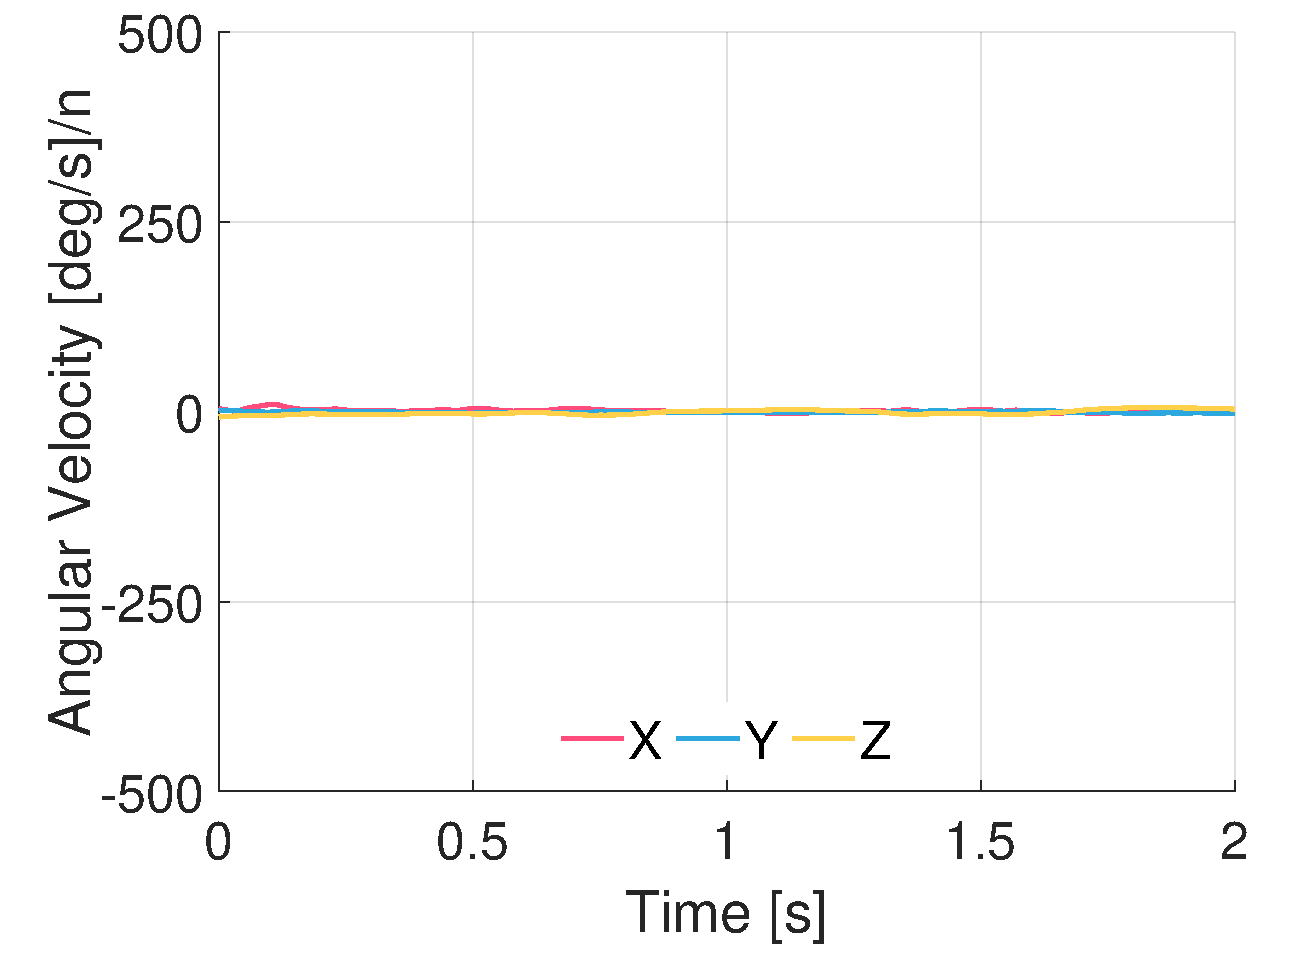
\includegraphics[width=\textwidth]{content/3-Methods/example-data/ch3_example_data_subject_01_l_ankle_gyro_activity_stop.pdf}
         \caption{Stopped}
    \end{subfigure}
    
    \begin{subfigure}[b]{0.49\textwidth}
         \centering
         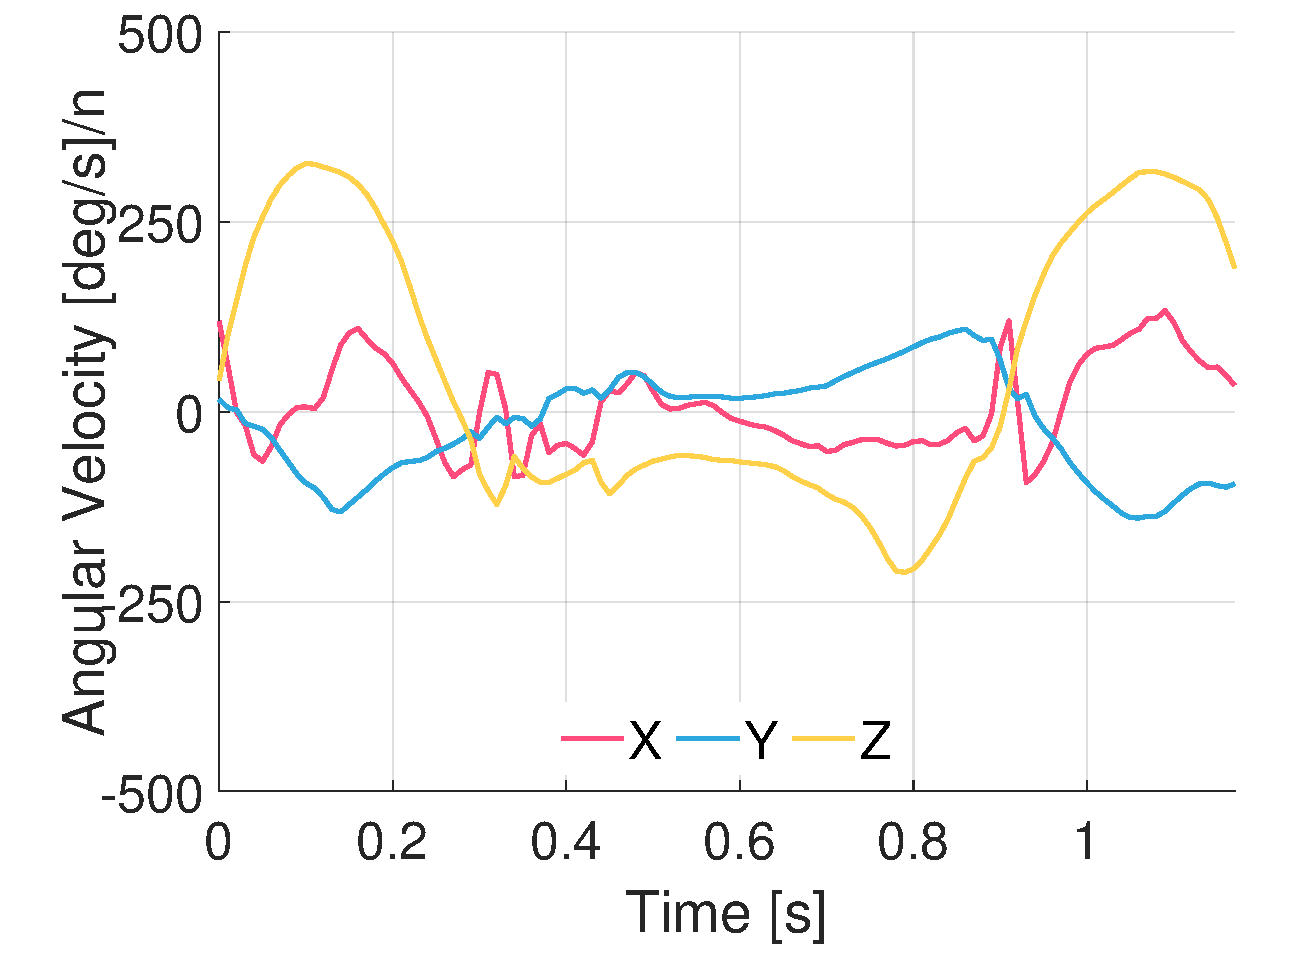
\includegraphics[width=\textwidth]{content/3-Methods/example-data/ch3_example_data_subject_01_l_ankle_gyro_activity_stair_down.pdf}
         \caption{Stair Ascent}
    \end{subfigure}
    \begin{subfigure}[b]{0.49\textwidth}
         \centering
         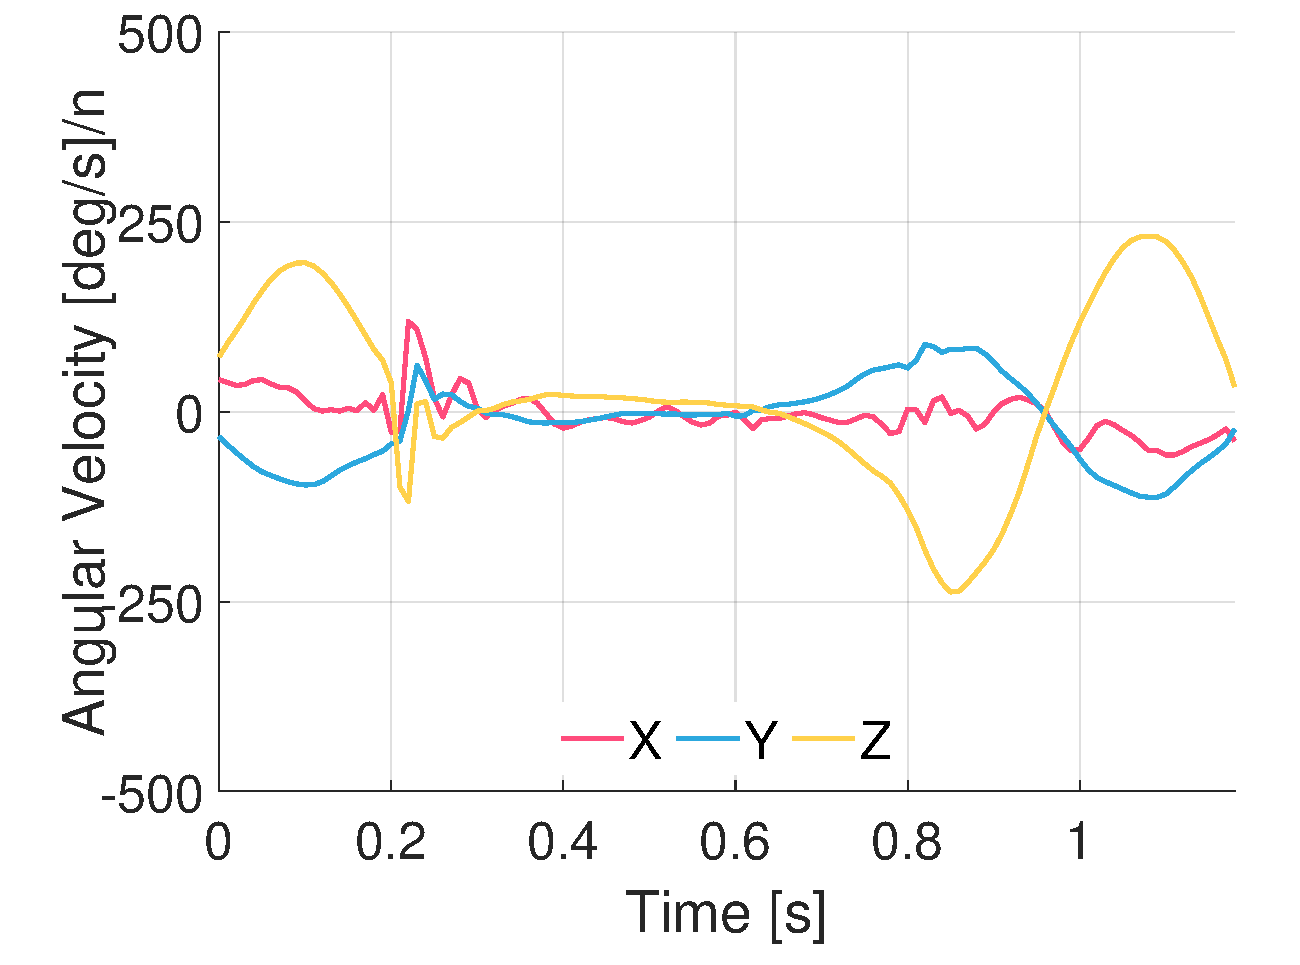
\includegraphics[width=\textwidth]{content/3-Methods/example-data/ch3_example_data_subject_01_l_ankle_gyro_activity_stair_up.pdf}
         \caption{Stair Descent}
    \end{subfigure}
    
    \begin{subfigure}[b]{0.49\textwidth}
         \centering
         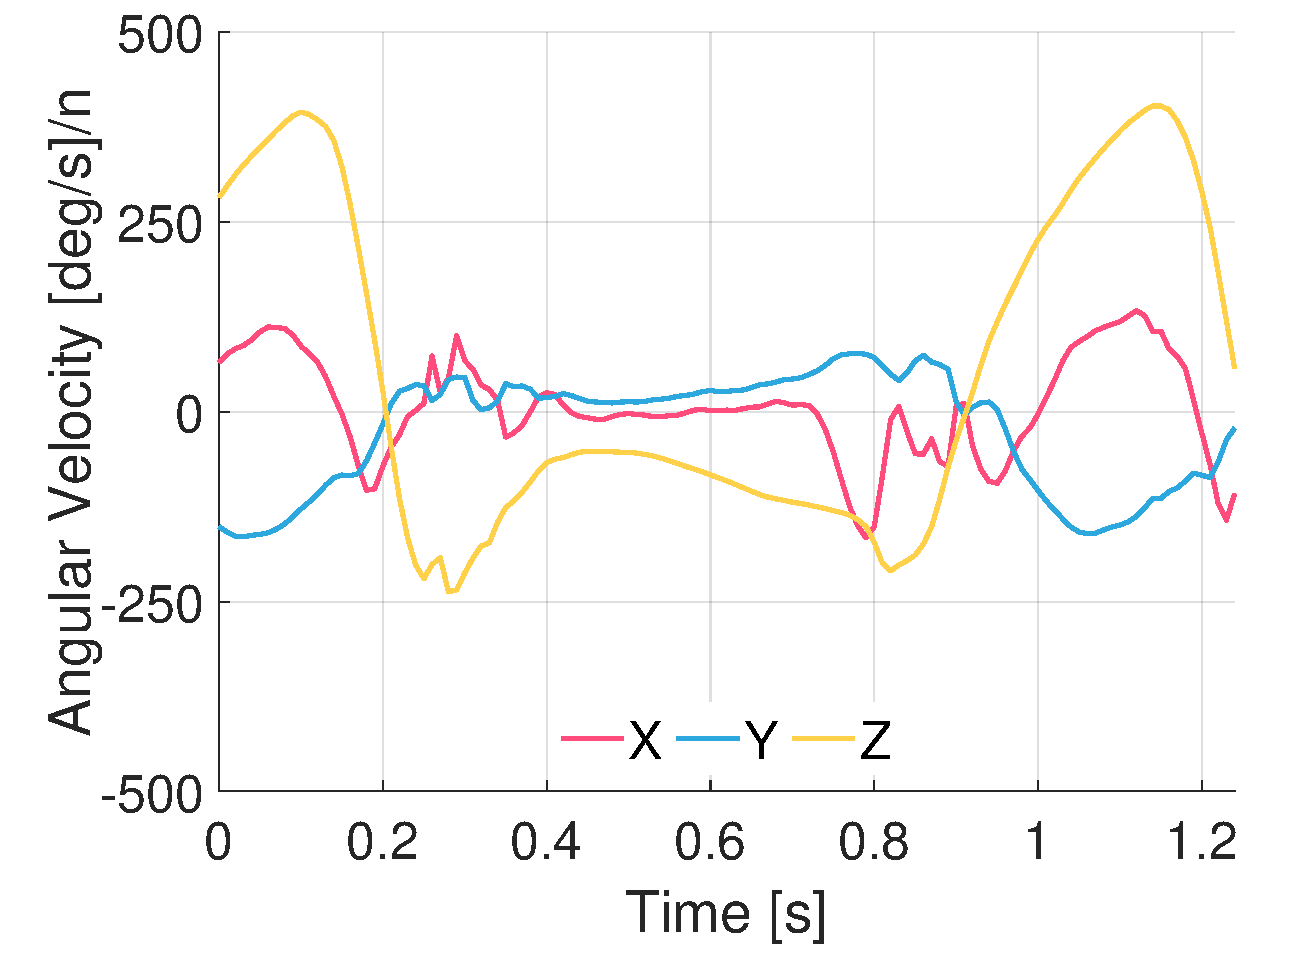
\includegraphics[width=\textwidth]{content/3-Methods/example-data/ch3_example_data_subject_01_l_ankle_gyro_activity_ramp_up.pdf}
         \caption{Ramp Ascent}
    \end{subfigure}
    \begin{subfigure}[b]{0.49\textwidth}
         \centering
         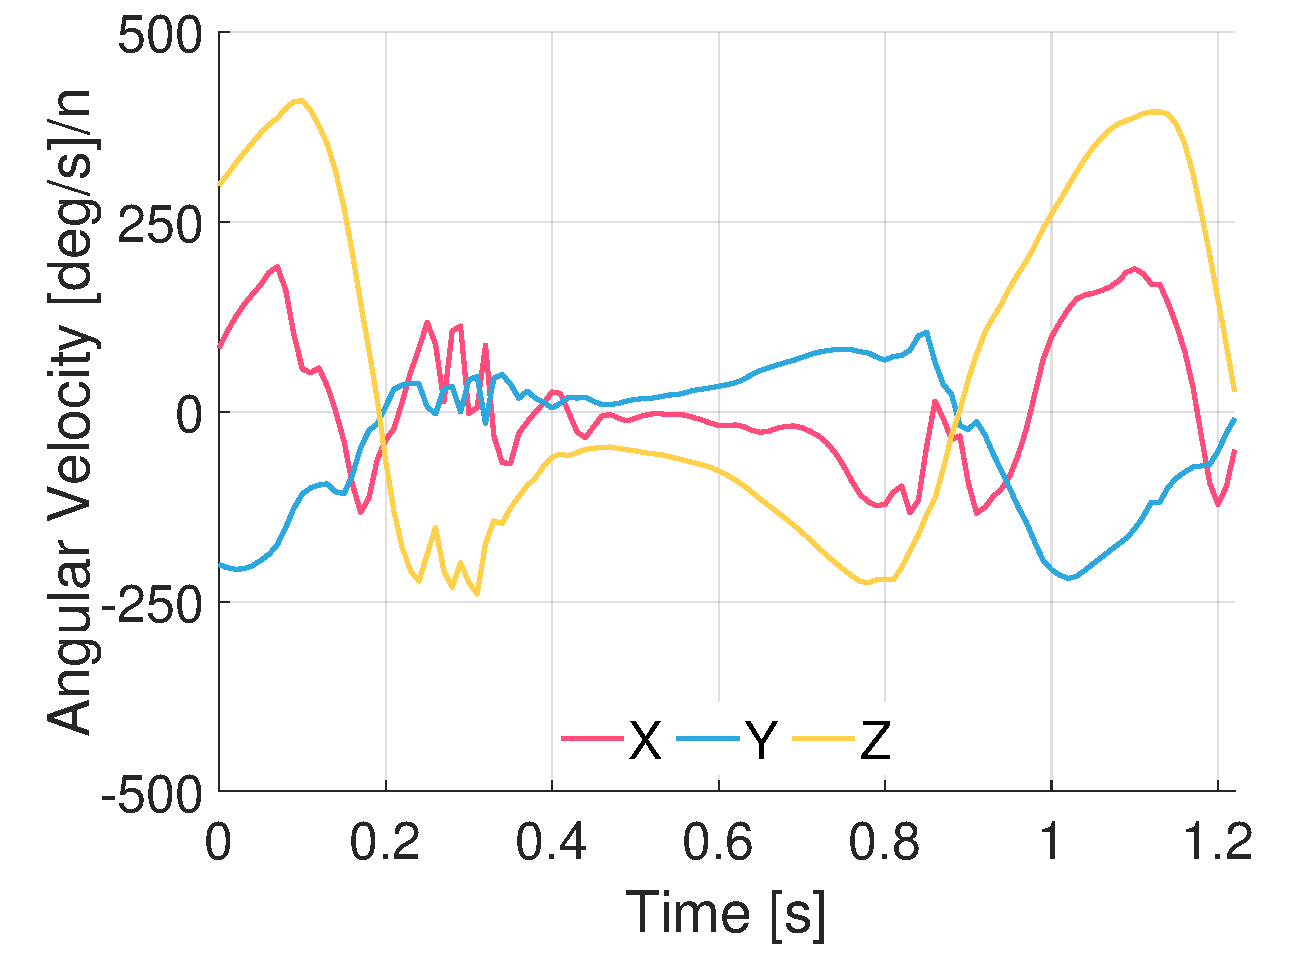
\includegraphics[width=\textwidth]{content/3-Methods/example-data/ch3_example_data_subject_01_l_ankle_gyro_activity_ramp_down.pdf}
         \caption{Ramp Descent}
    \end{subfigure}
    \caption[Example left ankle gyroscope data]{Example data for the left ankle gyroscope. The $x$ represent recording time in seconds. The y axis show the measured angular velocity in deg/s. The red lines represents the $x$ axis of the sensor, the blue solid lines the $y$ axis and the yellow lines the $z$ axis.}
    \label{fig:example-left-ankle-gyro-sensor-data}
\end{figure}

%---------------------- RIGHT ANKLE ------------------------
% Right Ankle - Accelerometer data
\begin{figure}[p]
\centering
    \begin{subfigure}[b]{0.49\textwidth}
         \centering
         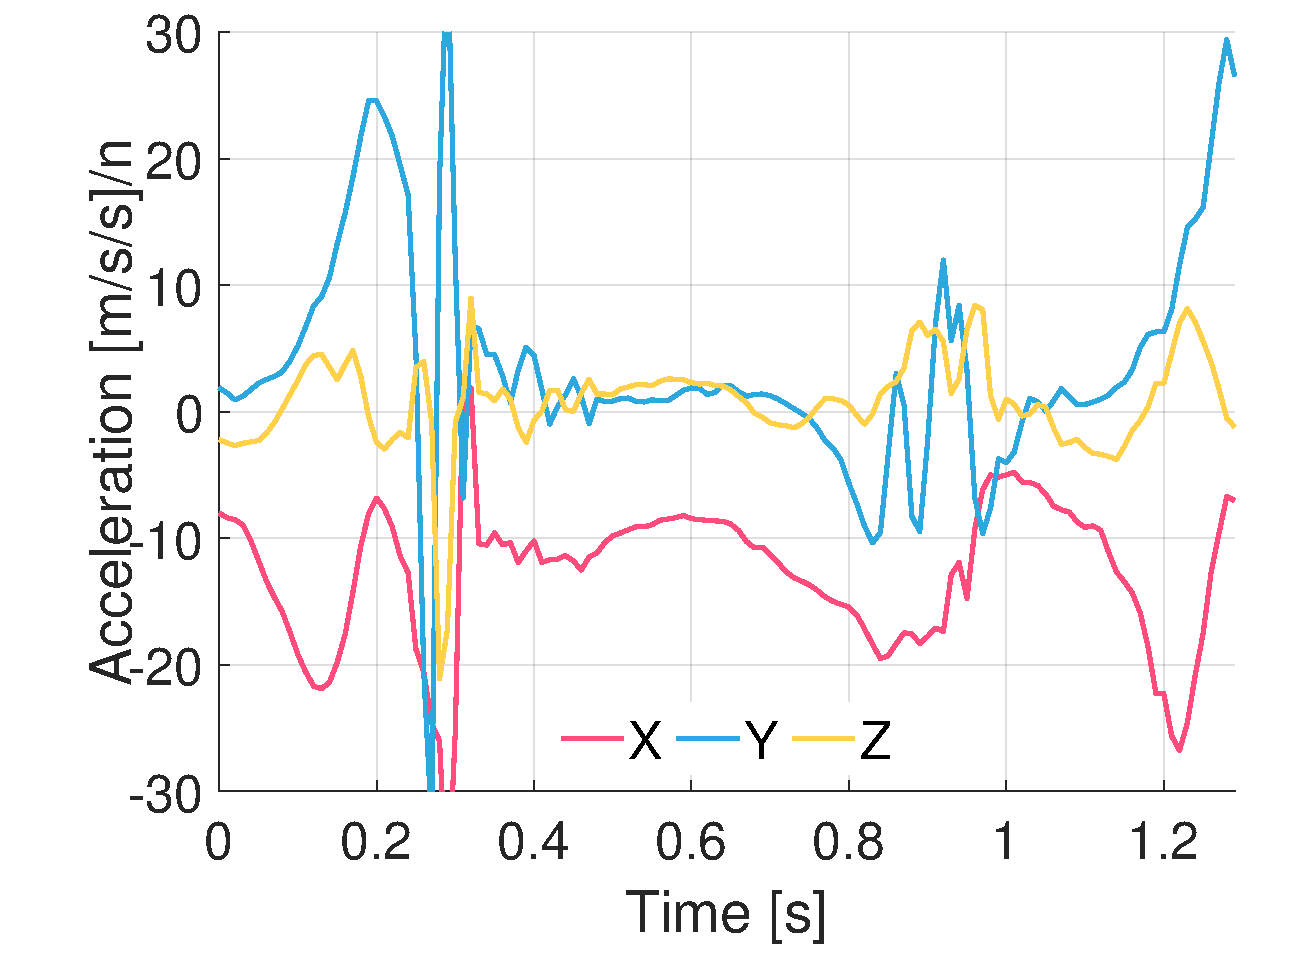
\includegraphics[width=\textwidth]{content/3-Methods/example-data/ch3_example_data_subject_01_r_ankle_accel_activity_walking.pdf}
         \caption{Walking}
    \end{subfigure}
    \begin{subfigure}[b]{0.49\textwidth}
         \centering
         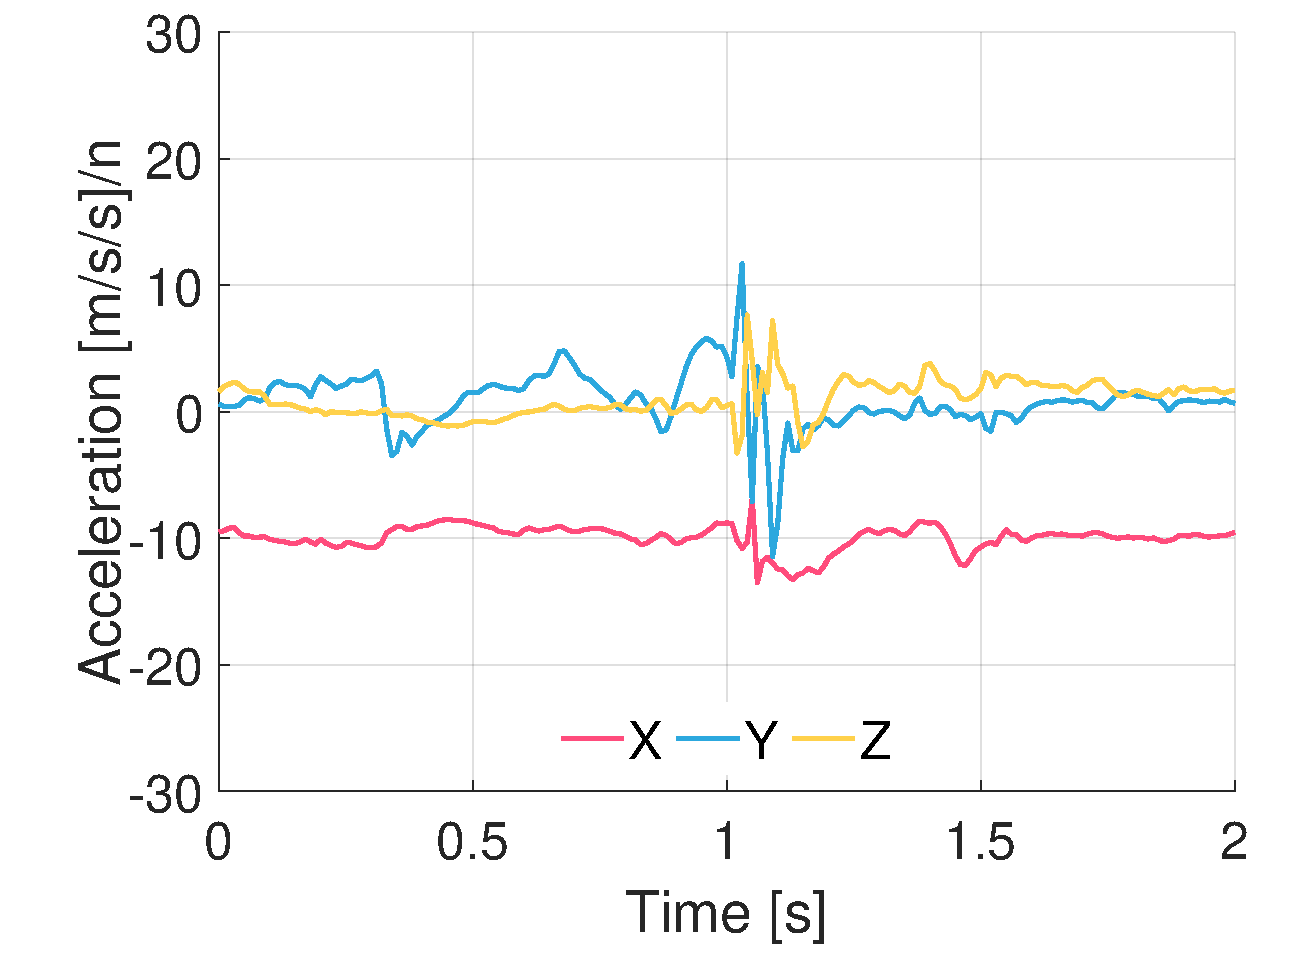
\includegraphics[width=\textwidth]{content/3-Methods/example-data/ch3_example_data_subject_01_r_ankle_accel_activity_stop.pdf}
         \caption{Stopped}
    \end{subfigure}
    
    \begin{subfigure}[b]{0.49\textwidth}
         \centering
         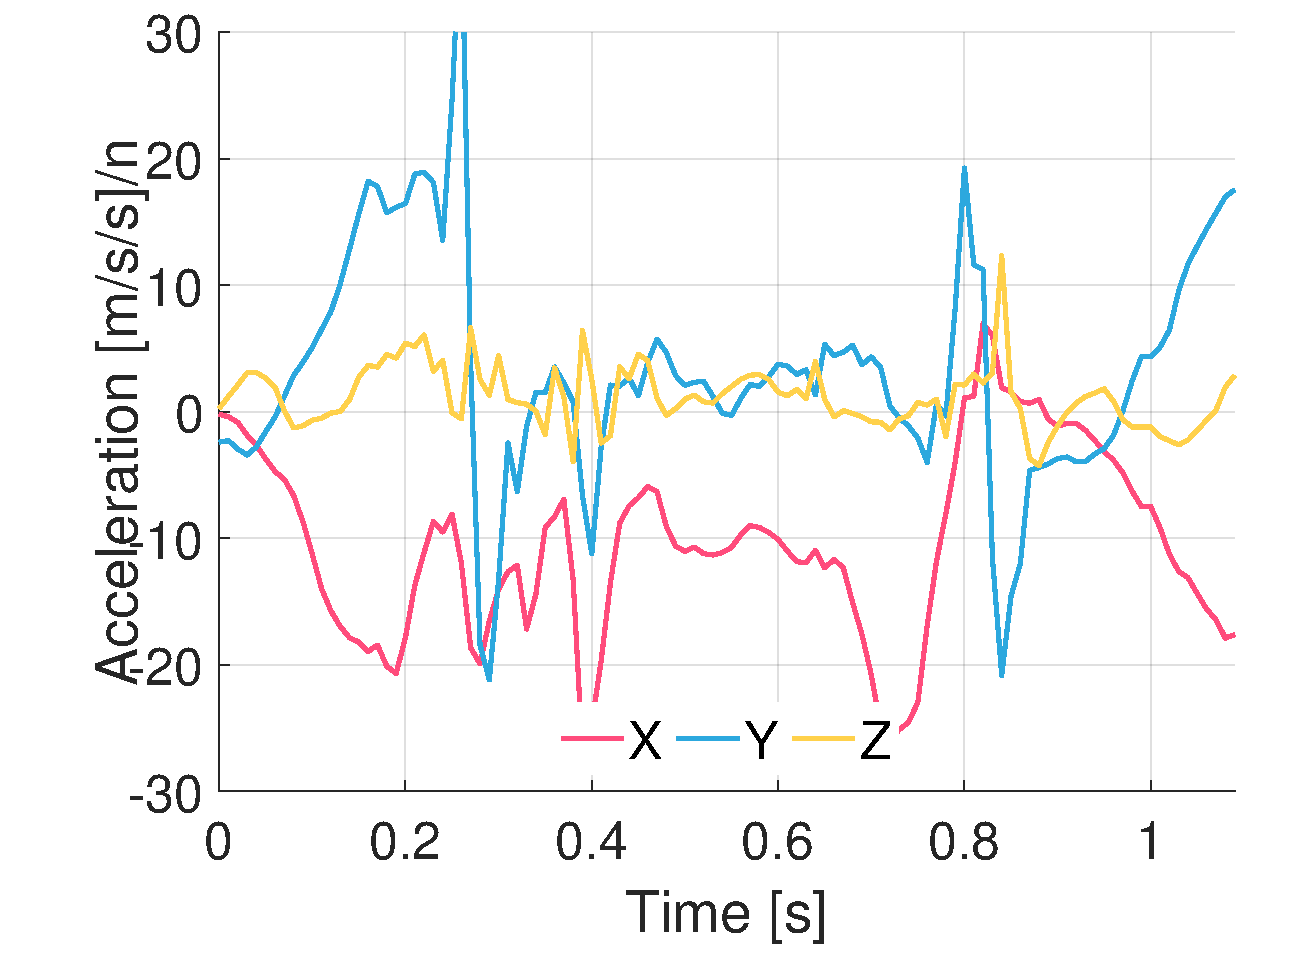
\includegraphics[width=\textwidth]{content/3-Methods/example-data/ch3_example_data_subject_01_r_ankle_accel_activity_stair_down.pdf}
         \caption{Stair Ascent}
    \end{subfigure}
    \begin{subfigure}[b]{0.49\textwidth}
         \centering
         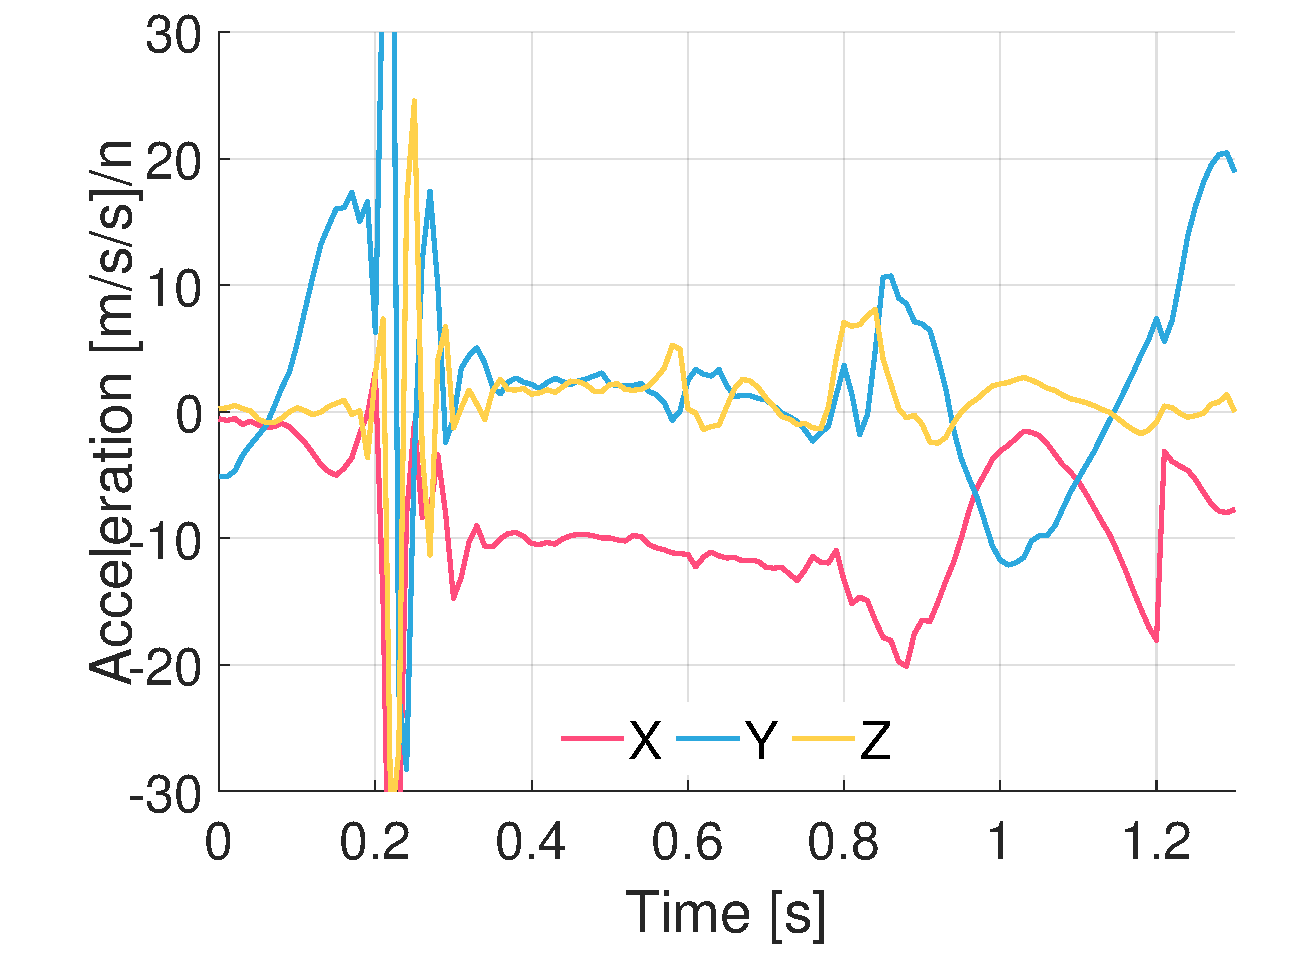
\includegraphics[width=\textwidth]{content/3-Methods/example-data/ch3_example_data_subject_01_r_ankle_accel_activity_stair_up.pdf}
         \caption{Stair Descent}
    \end{subfigure}
    
    \begin{subfigure}[b]{0.49\textwidth}
         \centering
         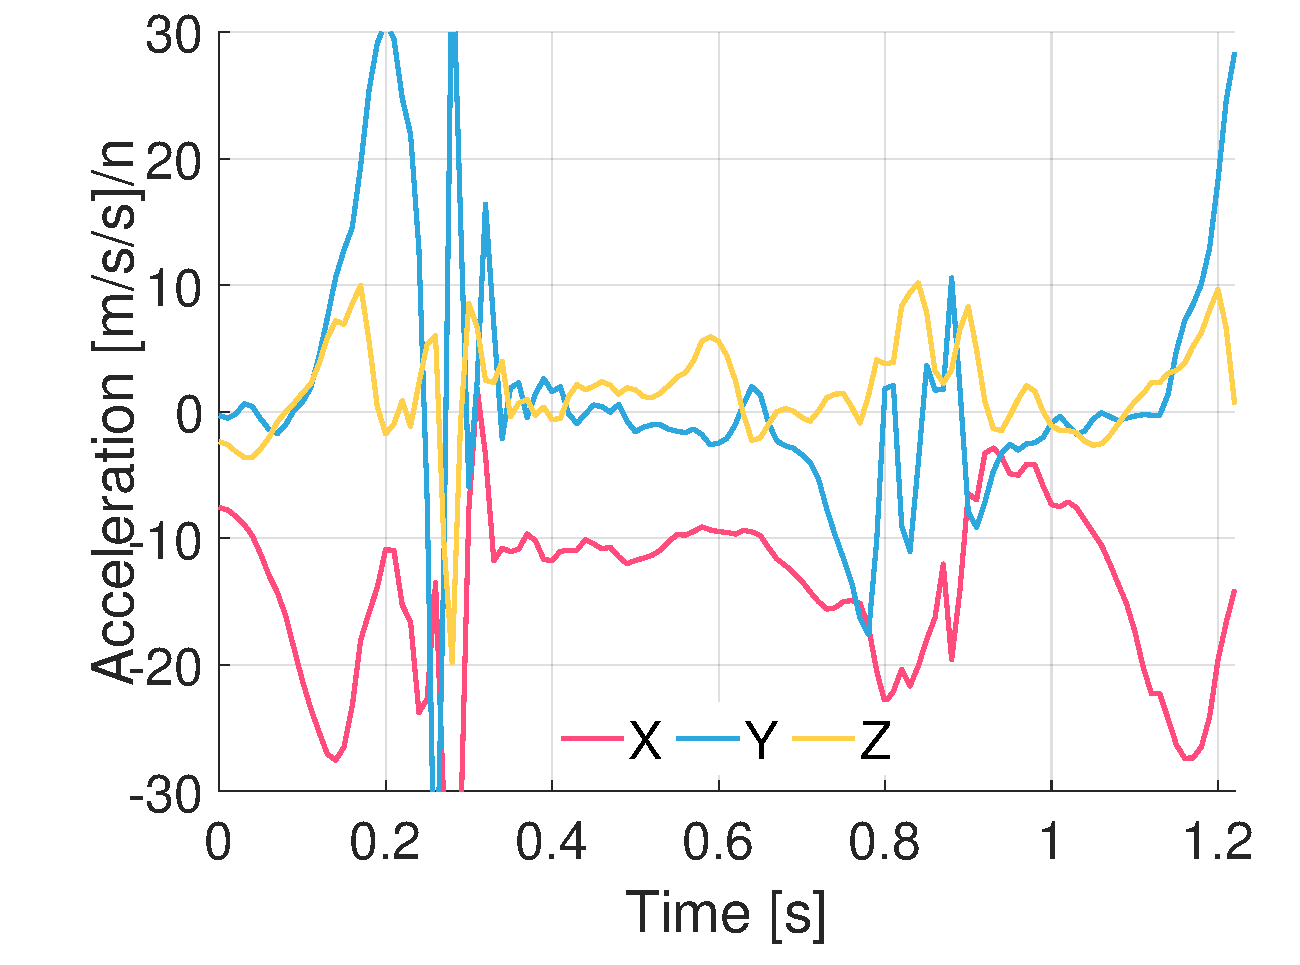
\includegraphics[width=\textwidth]{content/3-Methods/example-data/ch3_example_data_subject_01_r_ankle_accel_activity_ramp_up.pdf}
         \caption{Ramp Ascent}
    \end{subfigure}
    \begin{subfigure}[b]{0.49\textwidth}
         \centering
         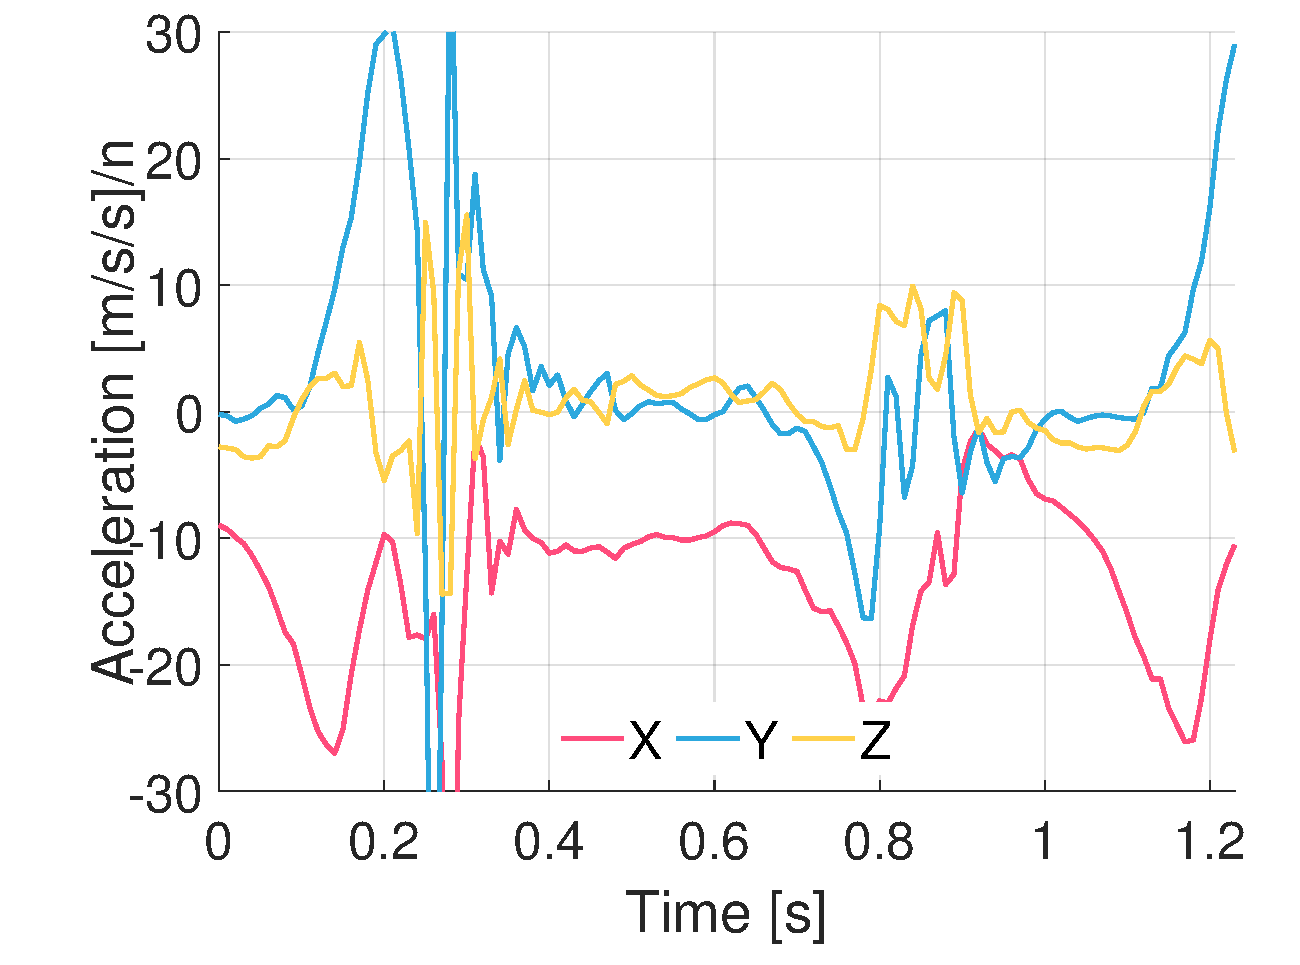
\includegraphics[width=\textwidth]{content/3-Methods/example-data/ch3_example_data_subject_01_r_ankle_accel_activity_ramp_down.pdf}
         \caption{Ramp Descent}
    \end{subfigure}
    \caption[Example right ankle accelerometer data]{Example data for the right ankle accelerometer. The $x$ represent recording time in seconds. The y axis show the measured acceleration in m/s/s. The red lines represents the $x$ axis of the sensor, the blue solid lines the $y$ axis and the yellow lines the $z$ axis.}
    \label{fig:example-right-ankle-accel-sensor-data}
\end{figure}

% Right ankle gyro
\begin{figure}[p]
\centering
    \begin{subfigure}[b]{0.49\textwidth}
         \centering
         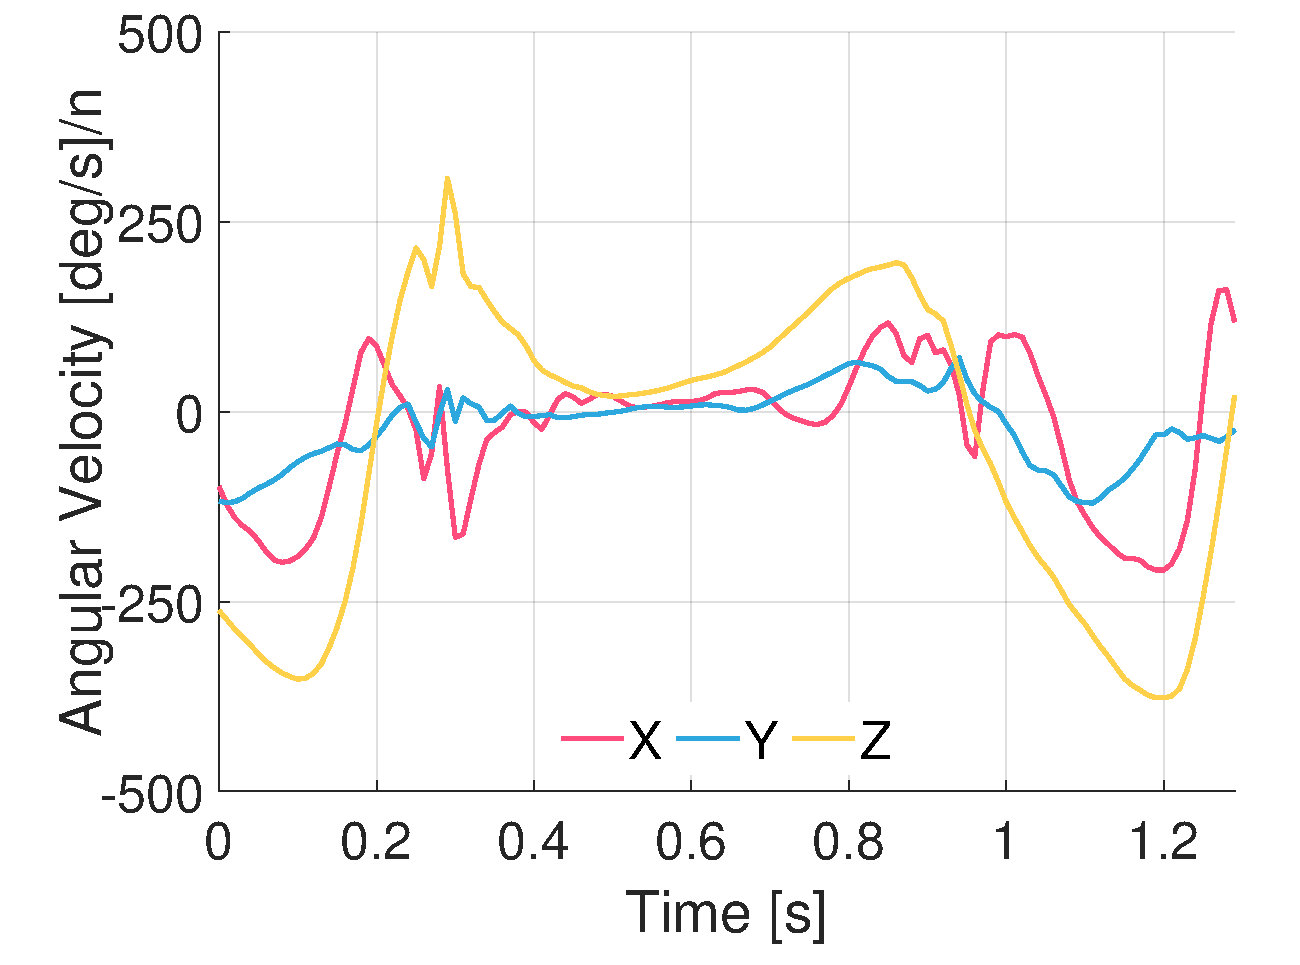
\includegraphics[width=\textwidth]{content/3-Methods/example-data/ch3_example_data_subject_01_r_ankle_gyro_activity_walking.pdf}
         \caption{Walking}
    \end{subfigure}
    \begin{subfigure}[b]{0.49\textwidth}
         \centering
         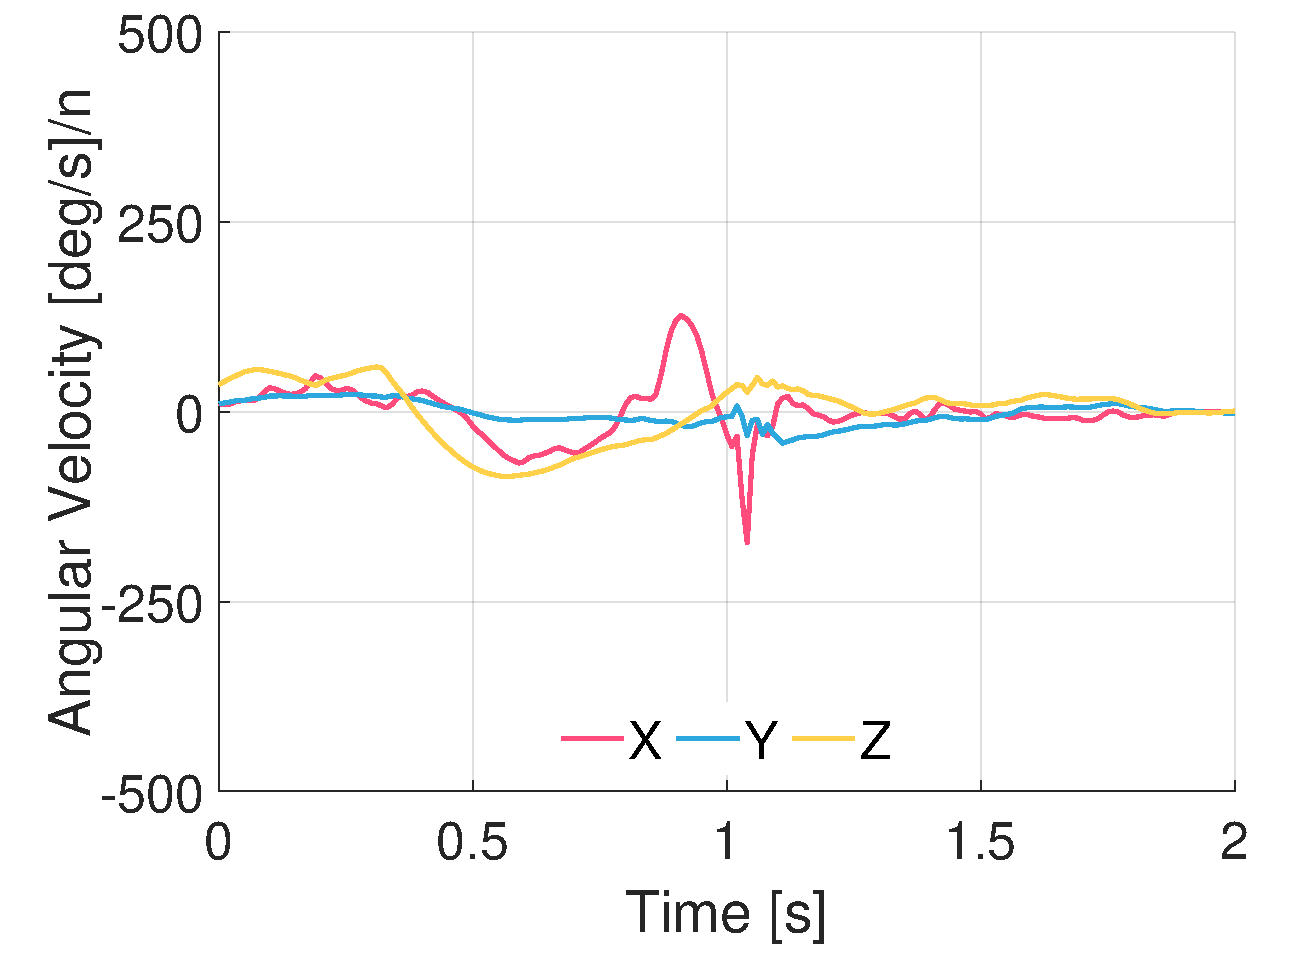
\includegraphics[width=\textwidth]{content/3-Methods/example-data/ch3_example_data_subject_01_r_ankle_gyro_activity_stop.pdf}
         \caption{Stopped}
    \end{subfigure}
    
    \begin{subfigure}[b]{0.49\textwidth}
         \centering
         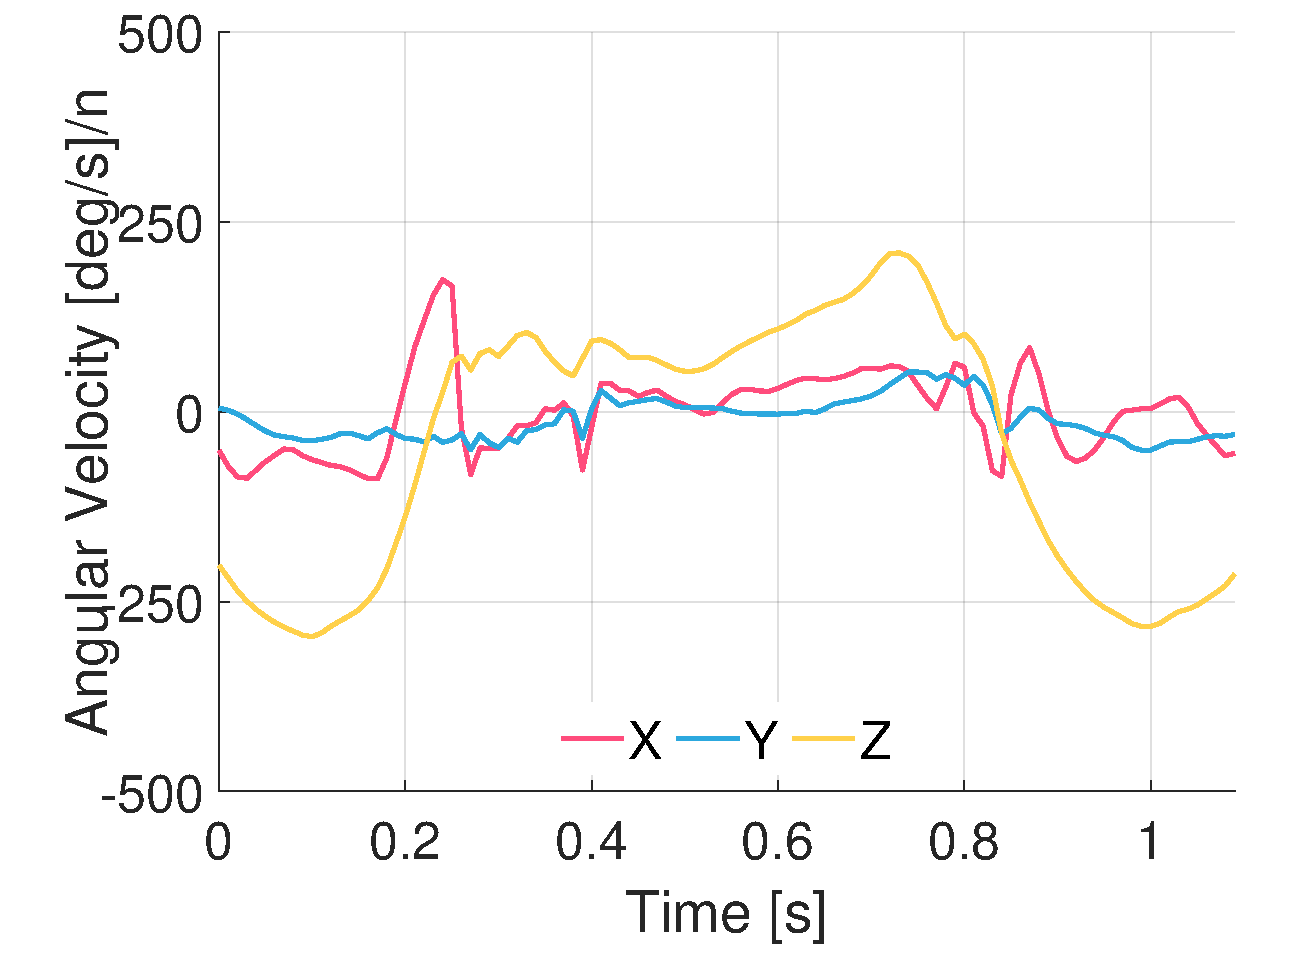
\includegraphics[width=\textwidth]{content/3-Methods/example-data/ch3_example_data_subject_01_r_ankle_gyro_activity_stair_down.pdf}
         \caption{Stair Ascent}
    \end{subfigure}
    \begin{subfigure}[b]{0.49\textwidth}
         \centering
         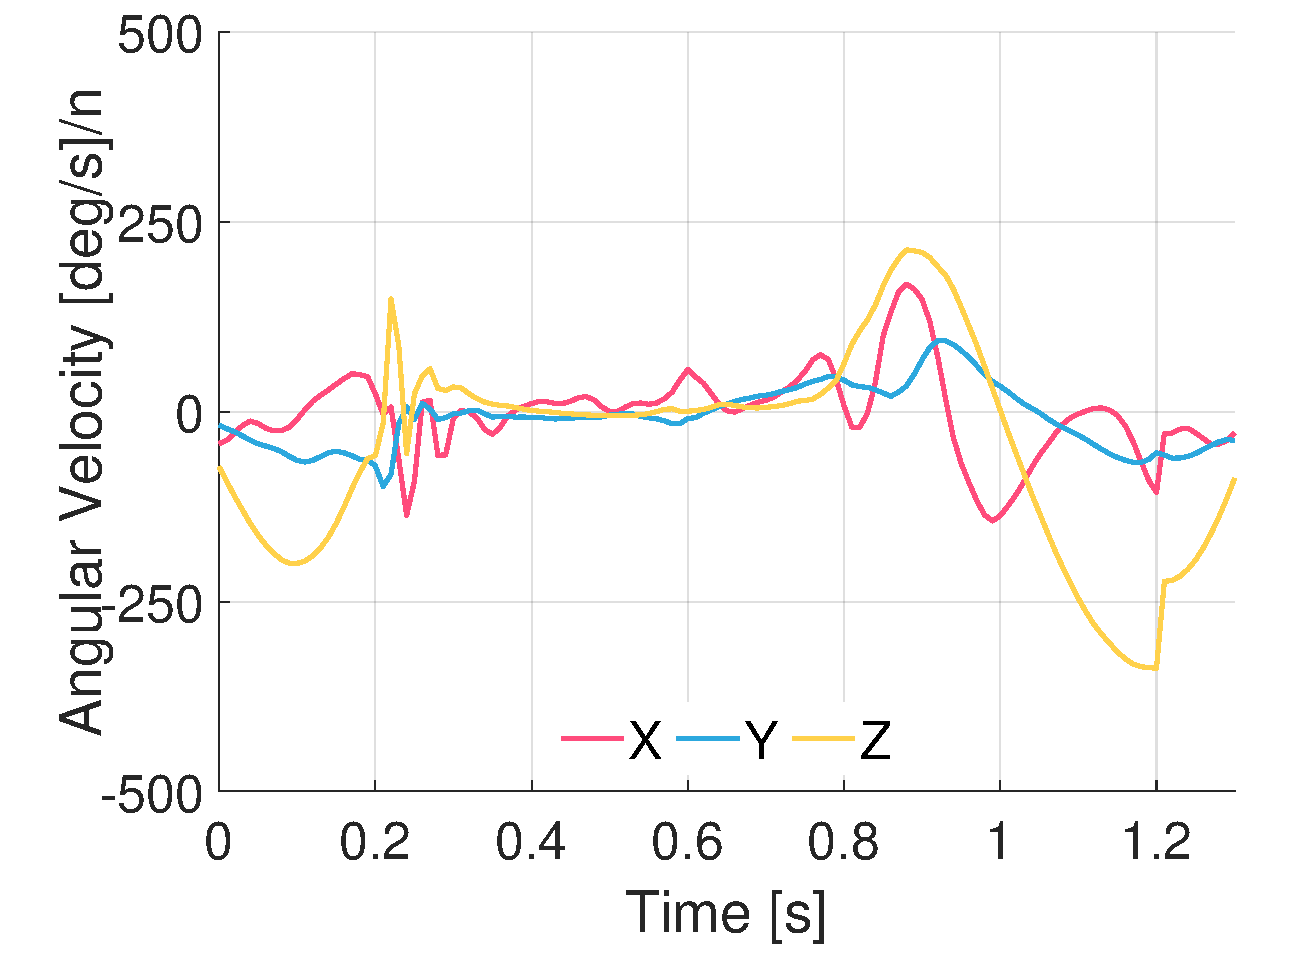
\includegraphics[width=\textwidth]{content/3-Methods/example-data/ch3_example_data_subject_01_r_ankle_gyro_activity_stair_up.pdf}
         \caption{Stair Descent}
    \end{subfigure}
    
    \begin{subfigure}[b]{0.49\textwidth}
         \centering
         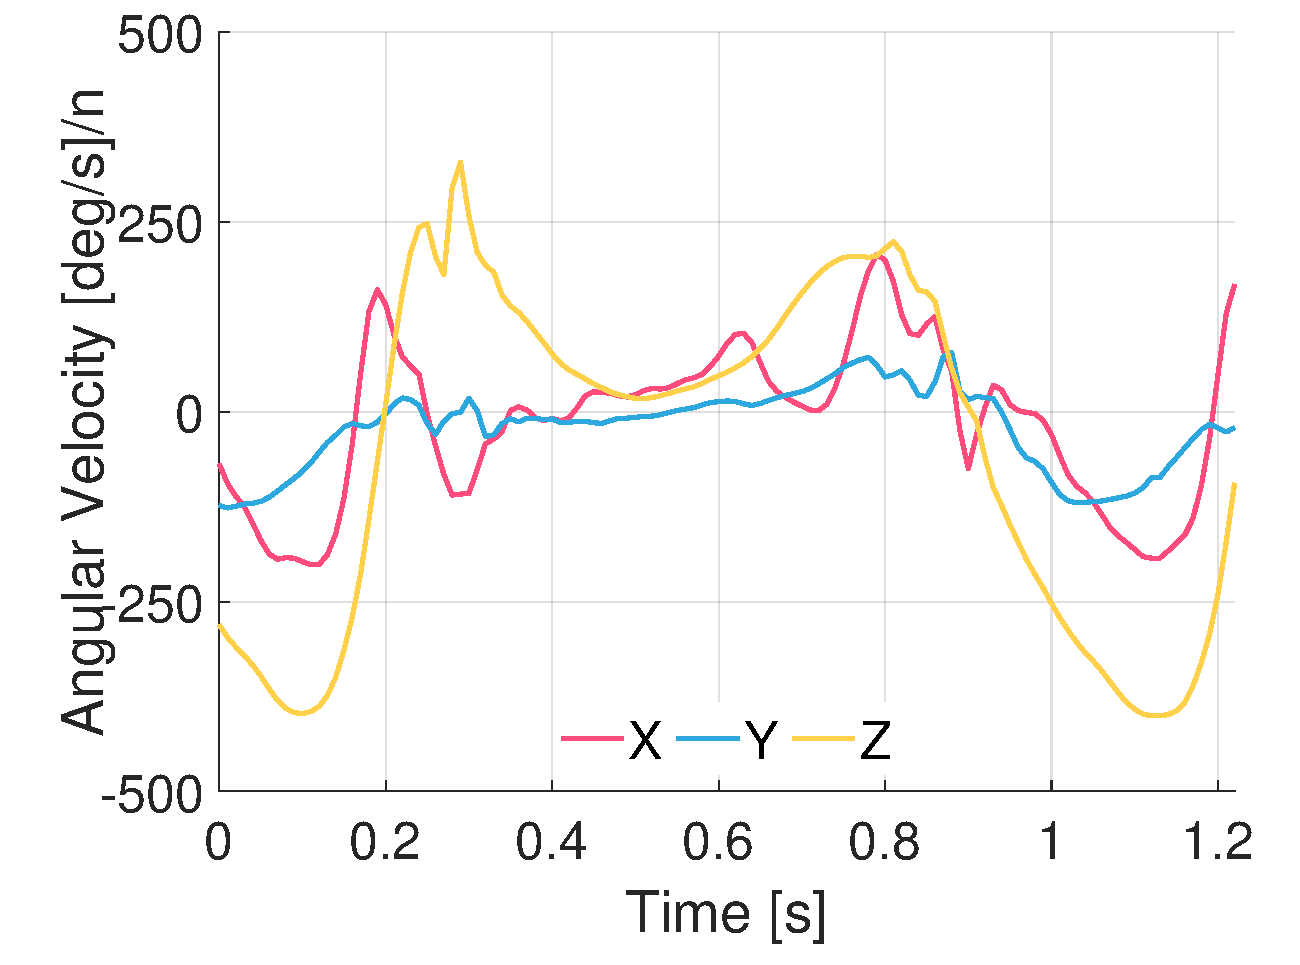
\includegraphics[width=\textwidth]{content/3-Methods/example-data/ch3_example_data_subject_01_r_ankle_gyro_activity_ramp_up.pdf}
         \caption{Ramp Ascent}
    \end{subfigure}
    \begin{subfigure}[b]{0.49\textwidth}
         \centering
         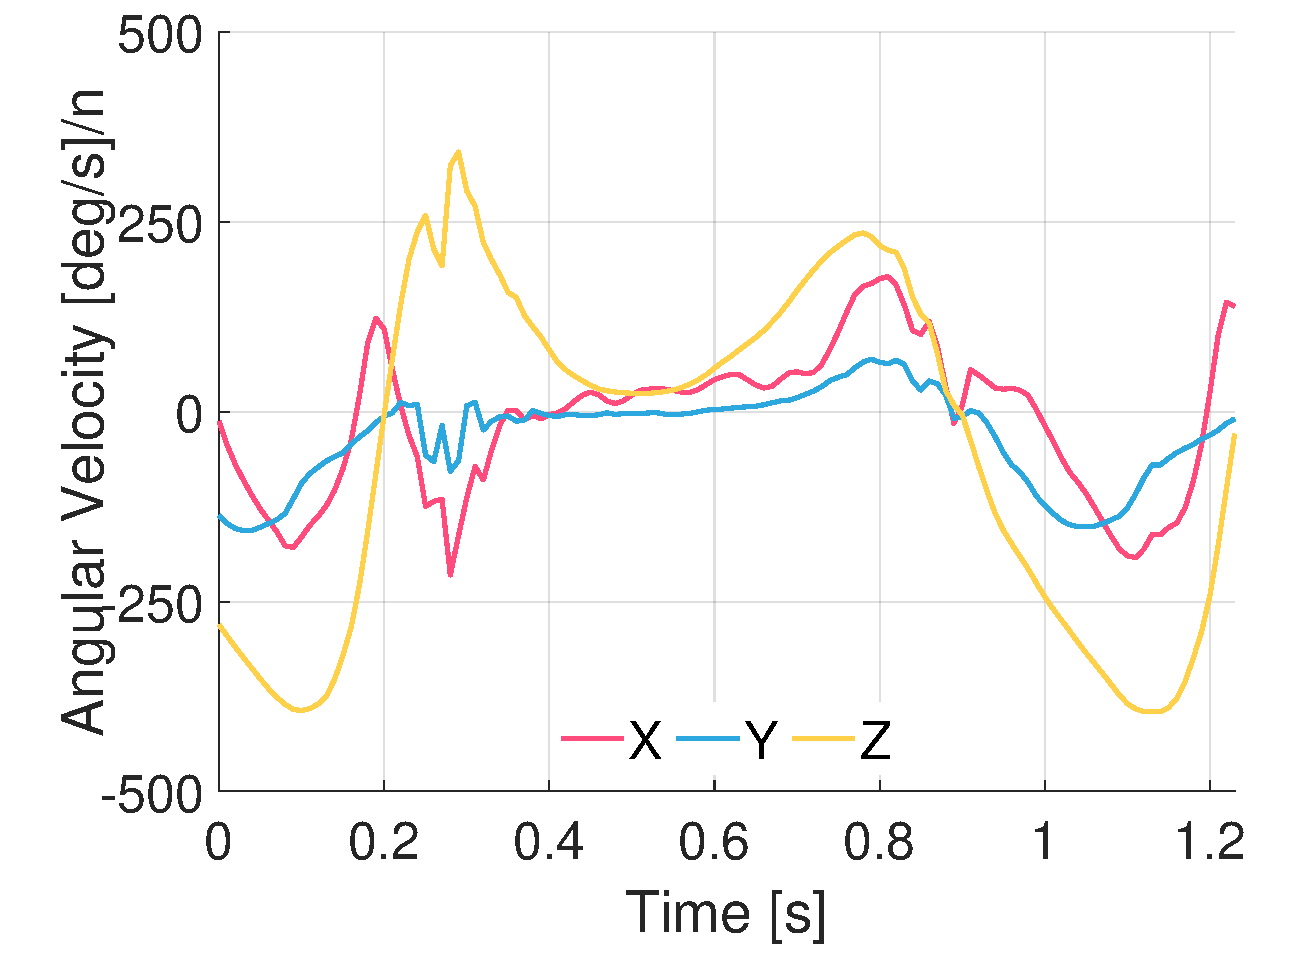
\includegraphics[width=\textwidth]{content/3-Methods/example-data/ch3_example_data_subject_01_r_ankle_gyro_activity_ramp_down.pdf}
         \caption{Ramp Descent}
    \end{subfigure}
    \caption[Example right ankle gyroscope data]{Example data for the right ankle gyroscope. The $x$ represent recording time in seconds. The y axis show the measured angular velocity in deg/s. The red lines represents the $x$ axis of the sensor, the blue solid lines the $y$ axis and the yellow lines the $z$ axis.}
    \label{fig:example-right-ankle-gyro-sensor-data}
\end{figure}

%---------------------- LEFT HIP ------------------------
% Left hip accelerometer
\begin{figure}[p]
\centering
    \begin{subfigure}[b]{0.49\textwidth}
         \centering
         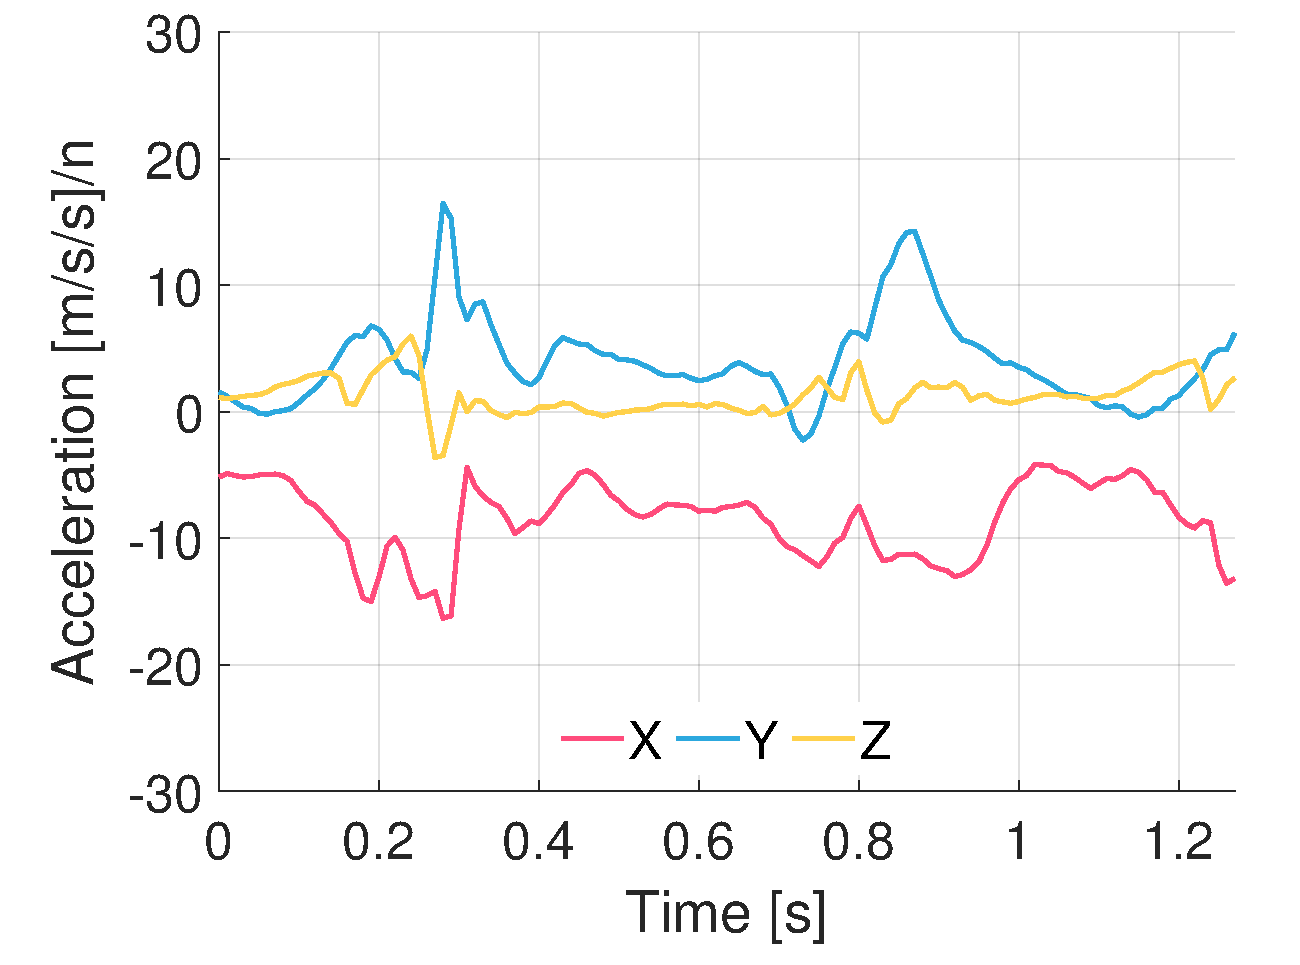
\includegraphics[width=\textwidth]{content/3-Methods/example-data/ch3_example_data_subject_01_l_hip_accel_activity_walking.pdf}
         \caption{Walking}
    \end{subfigure}
    \begin{subfigure}[b]{0.49\textwidth}
         \centering
         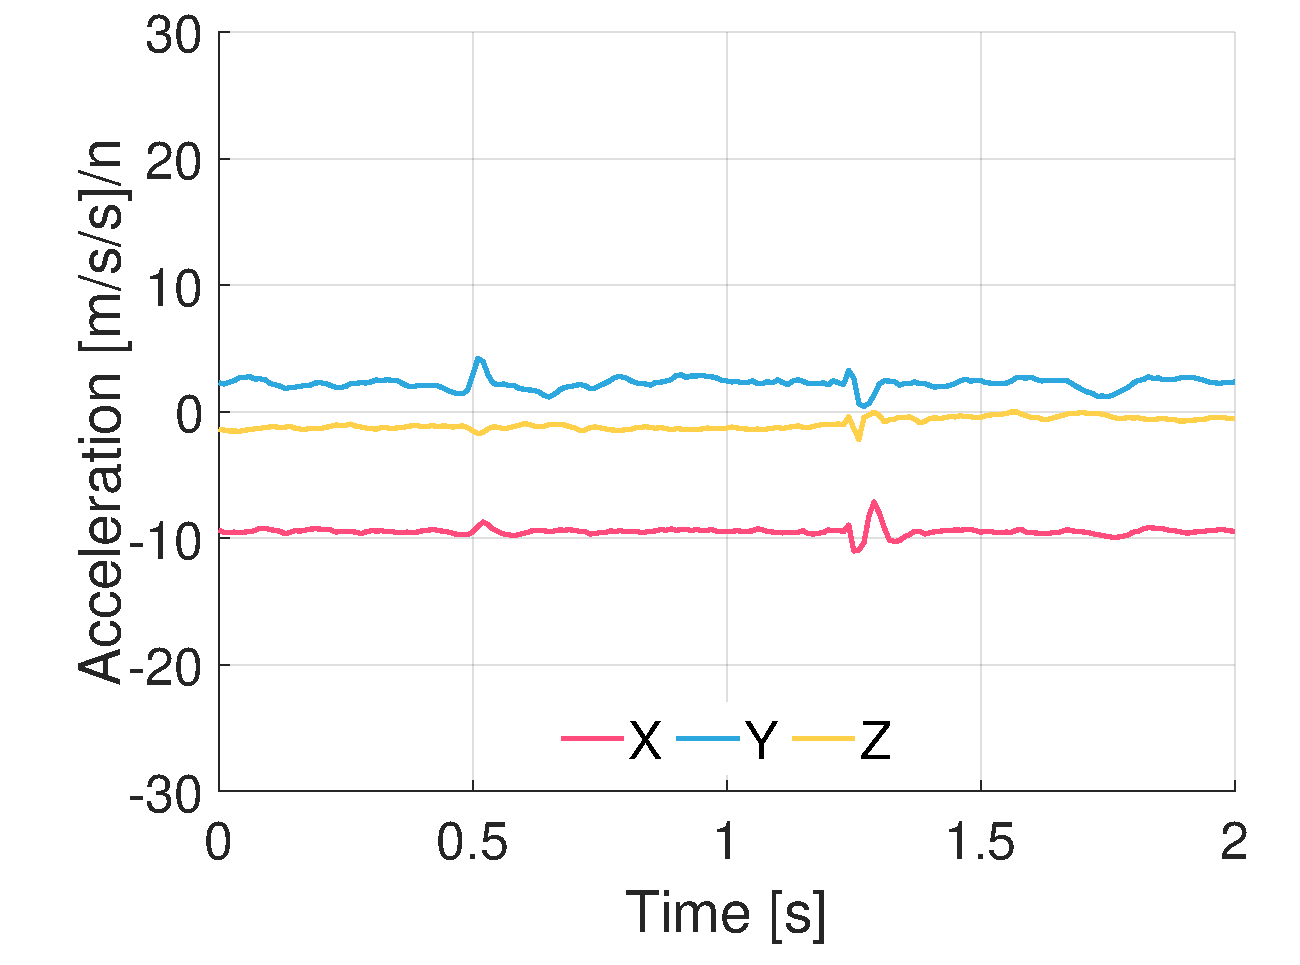
\includegraphics[width=\textwidth]{content/3-Methods/example-data/ch3_example_data_subject_01_l_hip_accel_activity_stop.pdf}
         \caption{Stopped}
    \end{subfigure}
    
    \begin{subfigure}[b]{0.49\textwidth}
         \centering
         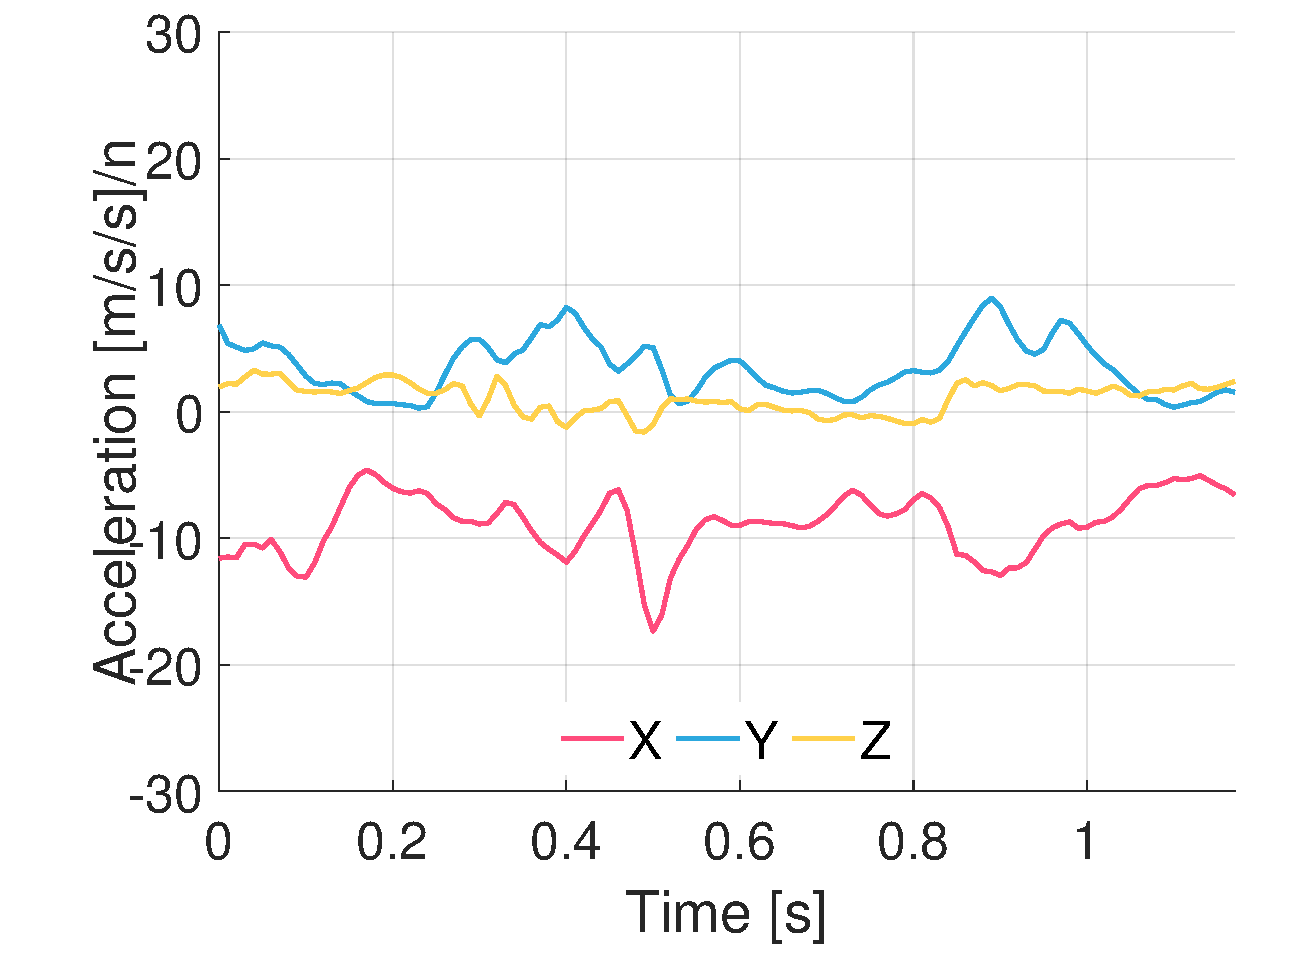
\includegraphics[width=\textwidth]{content/3-Methods/example-data/ch3_example_data_subject_01_l_hip_accel_activity_stair_down.pdf}
         \caption{Stair Ascent}
    \end{subfigure}
    \begin{subfigure}[b]{0.49\textwidth}
         \centering
         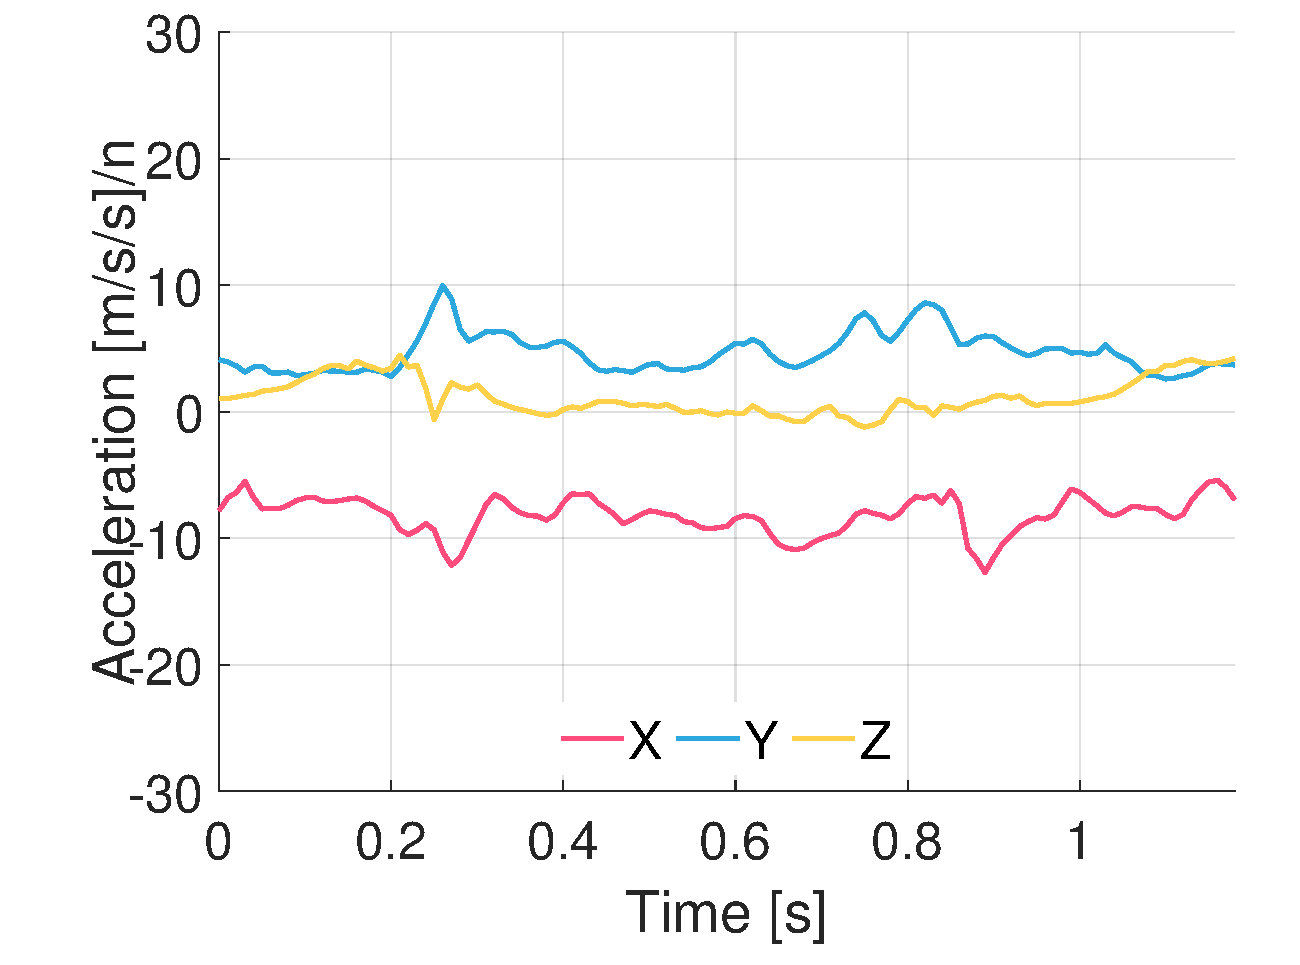
\includegraphics[width=\textwidth]{content/3-Methods/example-data/ch3_example_data_subject_01_l_hip_accel_activity_stair_up.pdf}
         \caption{Stair Descent}
    \end{subfigure}
    
    \begin{subfigure}[b]{0.49\textwidth}
         \centering
         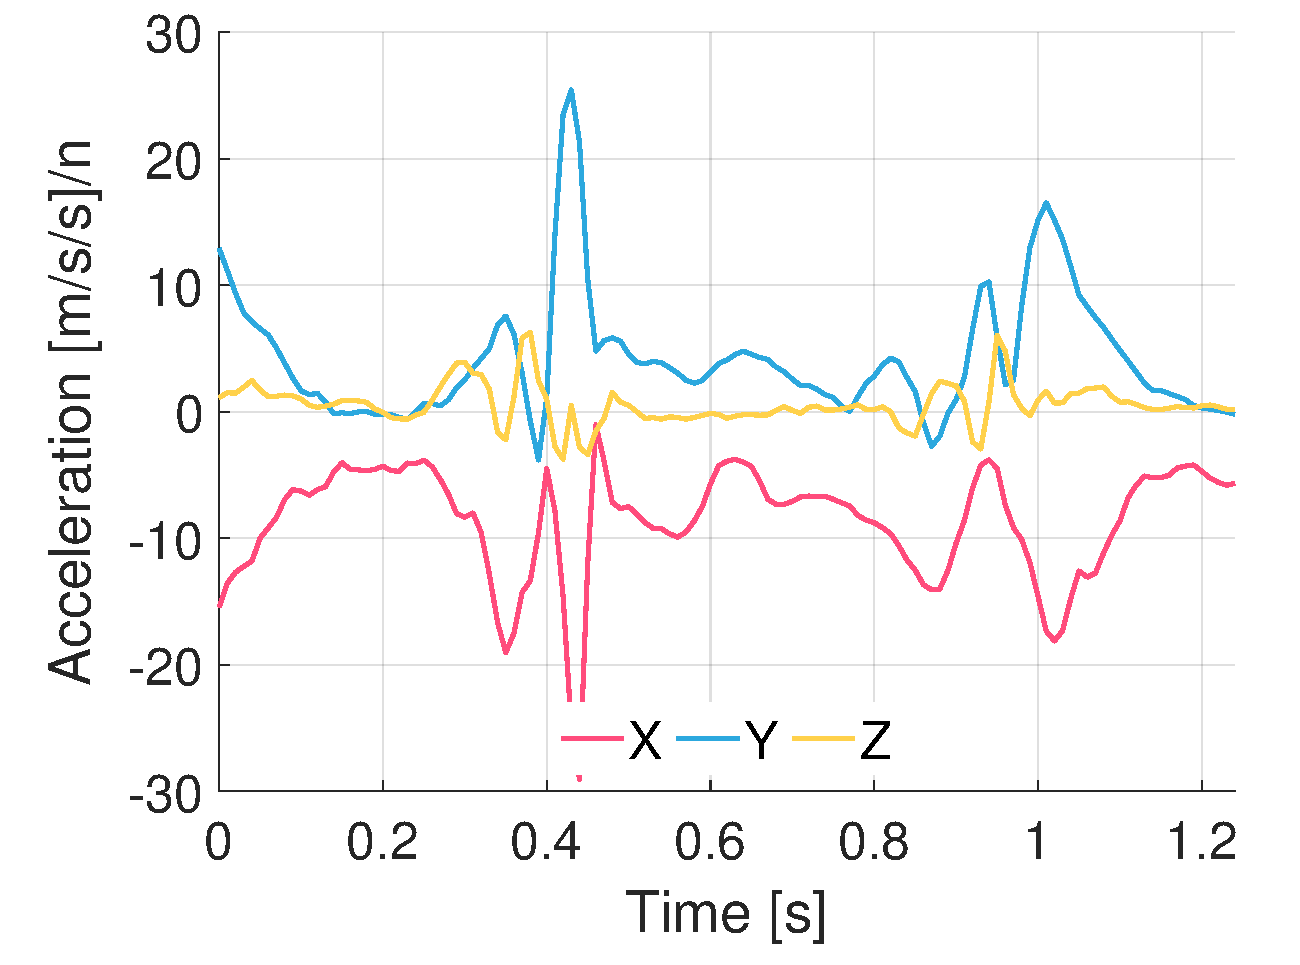
\includegraphics[width=\textwidth]{content/3-Methods/example-data/ch3_example_data_subject_01_l_hip_accel_activity_ramp_up.pdf}
         \caption{Ramp Ascent}
    \end{subfigure}
    \begin{subfigure}[b]{0.49\textwidth}
         \centering
         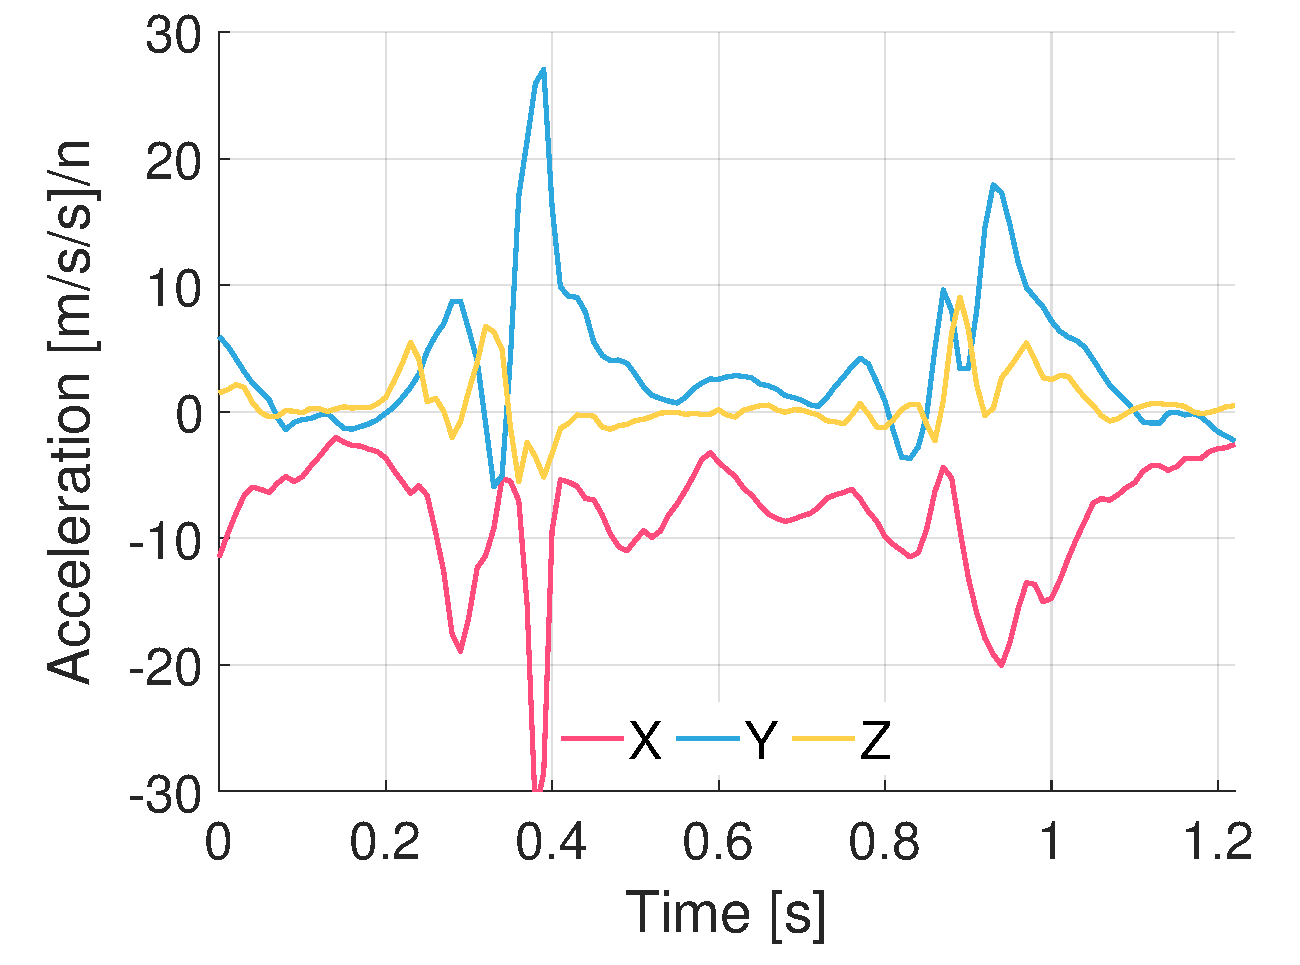
\includegraphics[width=\textwidth]{content/3-Methods/example-data/ch3_example_data_subject_01_l_hip_accel_activity_ramp_down.pdf}
         \caption{Ramp Descent}
    \end{subfigure}
    \caption[Example left hip accelerometer data]{Example data for the left hip accelerometer. The $x$ represent recording time in seconds. The y axis show the measured acceleration in m/s/s. The red lines represents the $x$ axis of the sensor, the blue solid lines the $y$ axis and the yellow lines the $z$ axis.}
    \label{fig:example-left-hip-accel-sensor-data}
\end{figure}

% Left hip gyro
\begin{figure}[p]
\centering
    \begin{subfigure}[b]{0.49\textwidth}
         \centering
         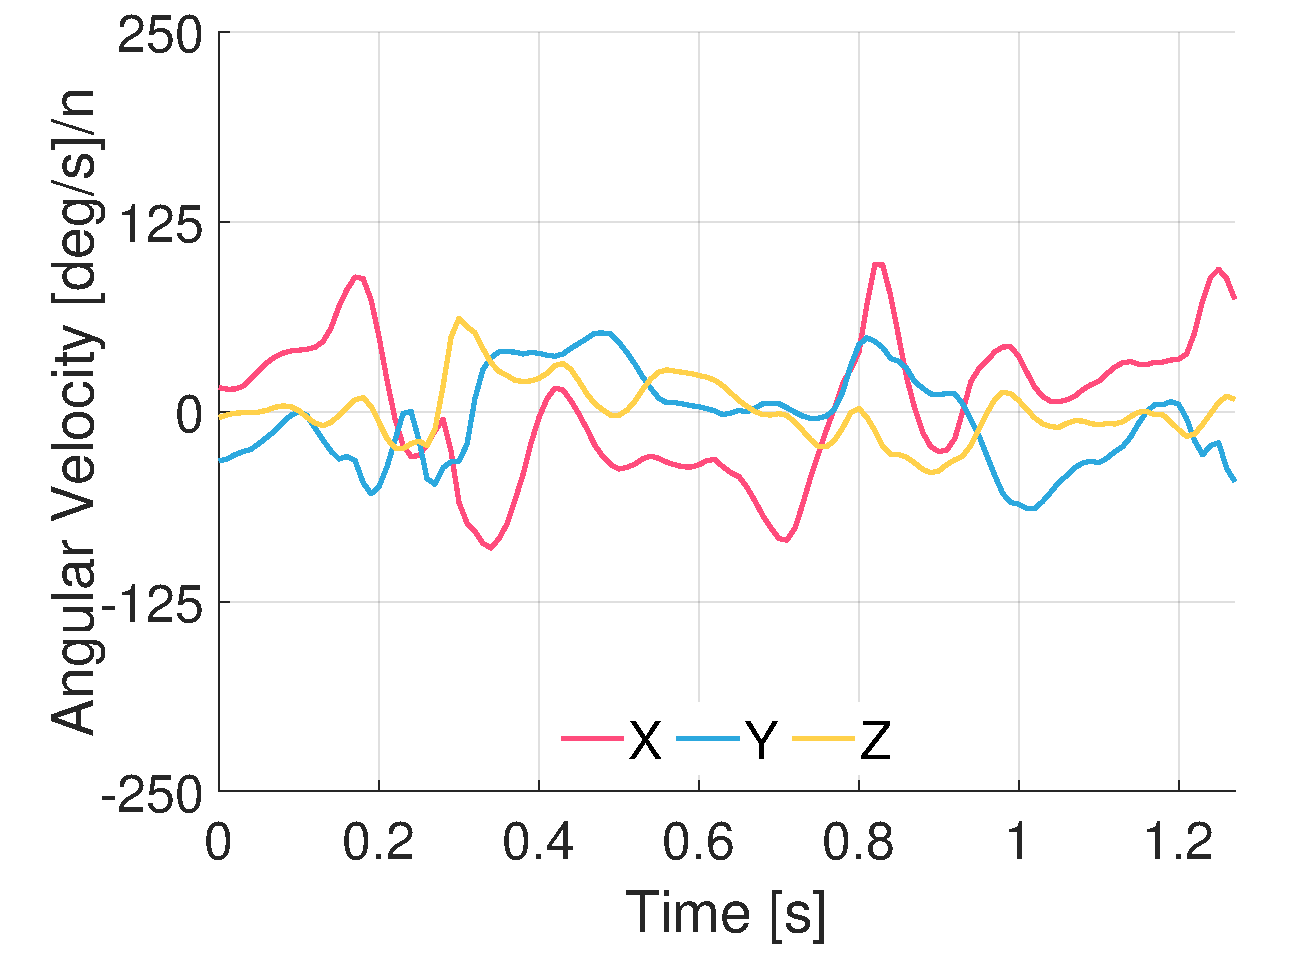
\includegraphics[width=\textwidth]{content/3-Methods/example-data/ch3_example_data_subject_01_l_hip_gyro_activity_walking.pdf}
         \caption{Walking}
    \end{subfigure}
    \begin{subfigure}[b]{0.49\textwidth}
         \centering
         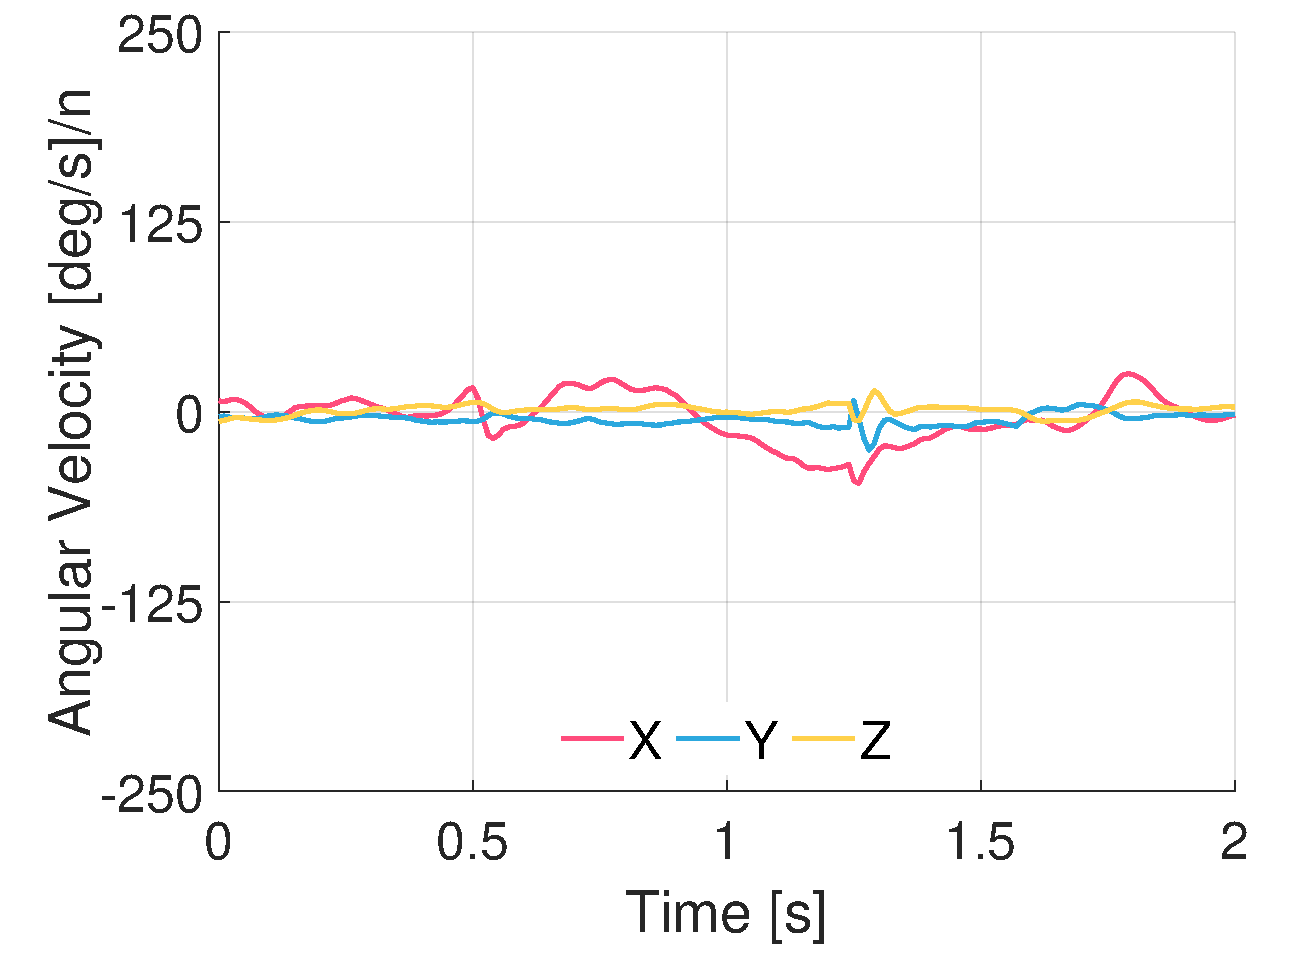
\includegraphics[width=\textwidth]{content/3-Methods/example-data/ch3_example_data_subject_01_l_hip_gyro_activity_stop.pdf}
         \caption{Stopped}
    \end{subfigure}
    
    \begin{subfigure}[b]{0.49\textwidth}
         \centering
         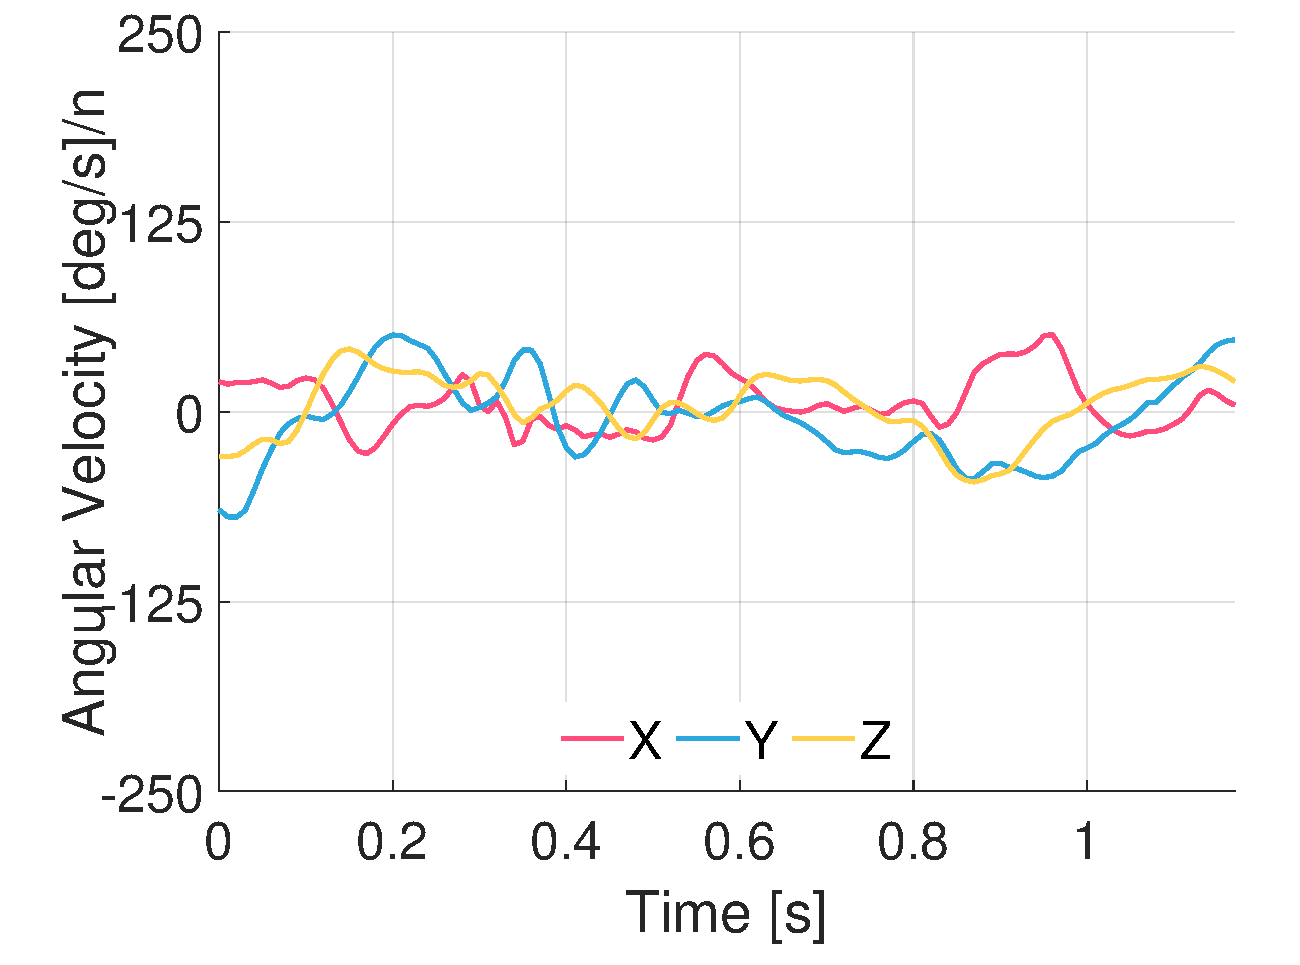
\includegraphics[width=\textwidth]{content/3-Methods/example-data/ch3_example_data_subject_01_l_hip_gyro_activity_stair_down.pdf}
         \caption{Stair Ascent}
    \end{subfigure}
    \begin{subfigure}[b]{0.49\textwidth}
         \centering
         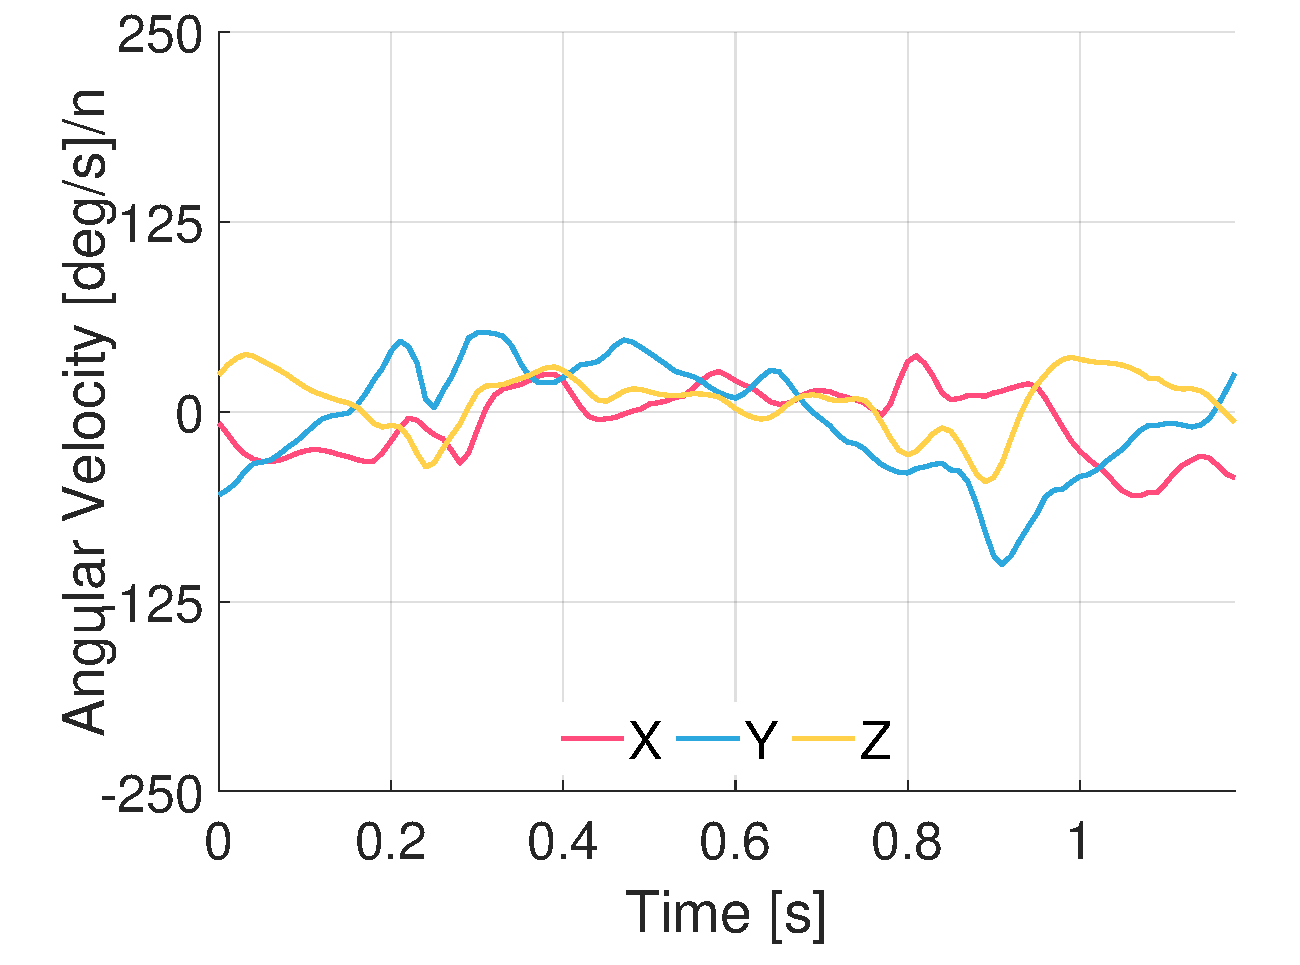
\includegraphics[width=\textwidth]{content/3-Methods/example-data/ch3_example_data_subject_01_l_hip_gyro_activity_stair_up.pdf}
         \caption{Stair Descent}
    \end{subfigure}
    
    \begin{subfigure}[b]{0.49\textwidth}
         \centering
         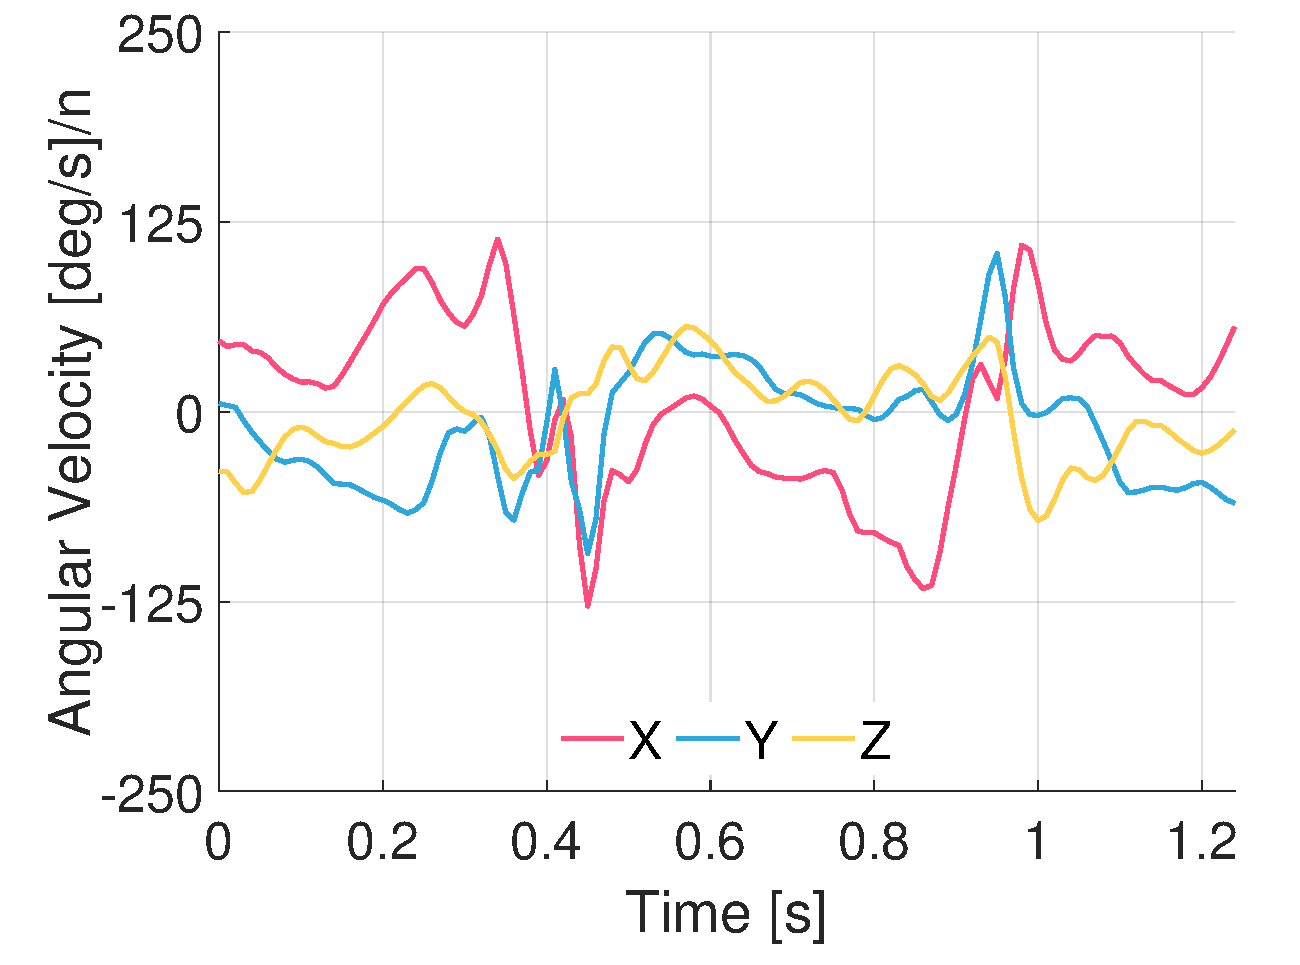
\includegraphics[width=\textwidth]{content/3-Methods/example-data/ch3_example_data_subject_01_l_hip_gyro_activity_ramp_up.pdf}
         \caption{Ramp Ascent}
    \end{subfigure}
    \begin{subfigure}[b]{0.49\textwidth}
         \centering
         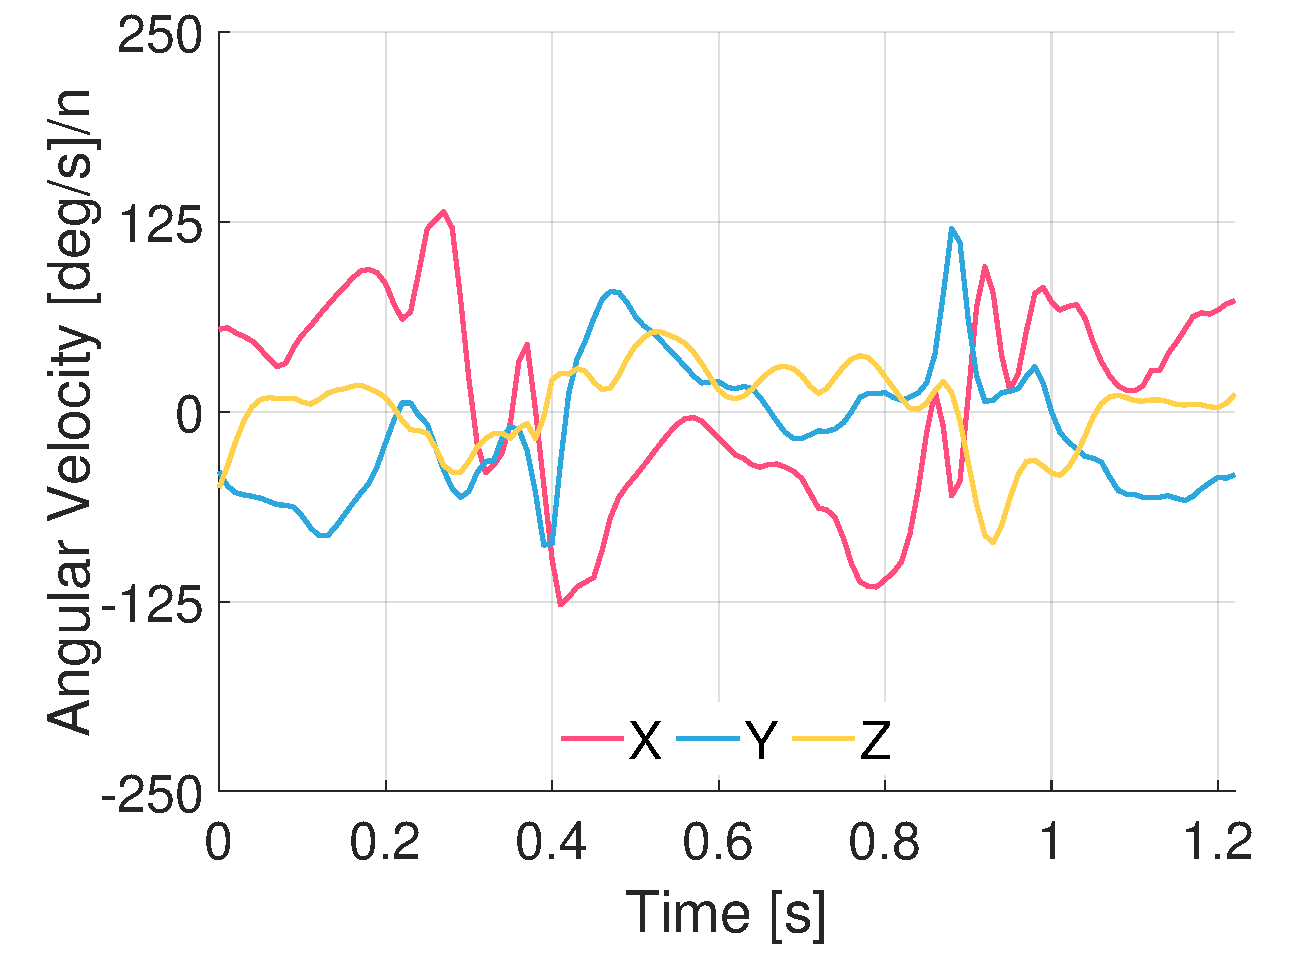
\includegraphics[width=\textwidth]{content/3-Methods/example-data/ch3_example_data_subject_01_l_hip_gyro_activity_ramp_down.pdf}
         \caption{Ramp Descent}
    \end{subfigure}
    \caption[Example left hip gyroscope data]{Example data for the left hip gyroscope. The $x$ represent recording time in seconds. The y axis show the measured angular velocity in deg/s. The red lines represents the $x$ axis of the sensor, the blue solid lines the $y$ axis and the yellow lines the $z$ axis.}
    \label{fig:example-left-hip-gyro-sensor-data}
\end{figure}

%---------------------- RIGHT HIP ------------------------
% right hip accelerometer
\begin{figure}[p]
\centering
    \begin{subfigure}[b]{0.49\textwidth}
         \centering
         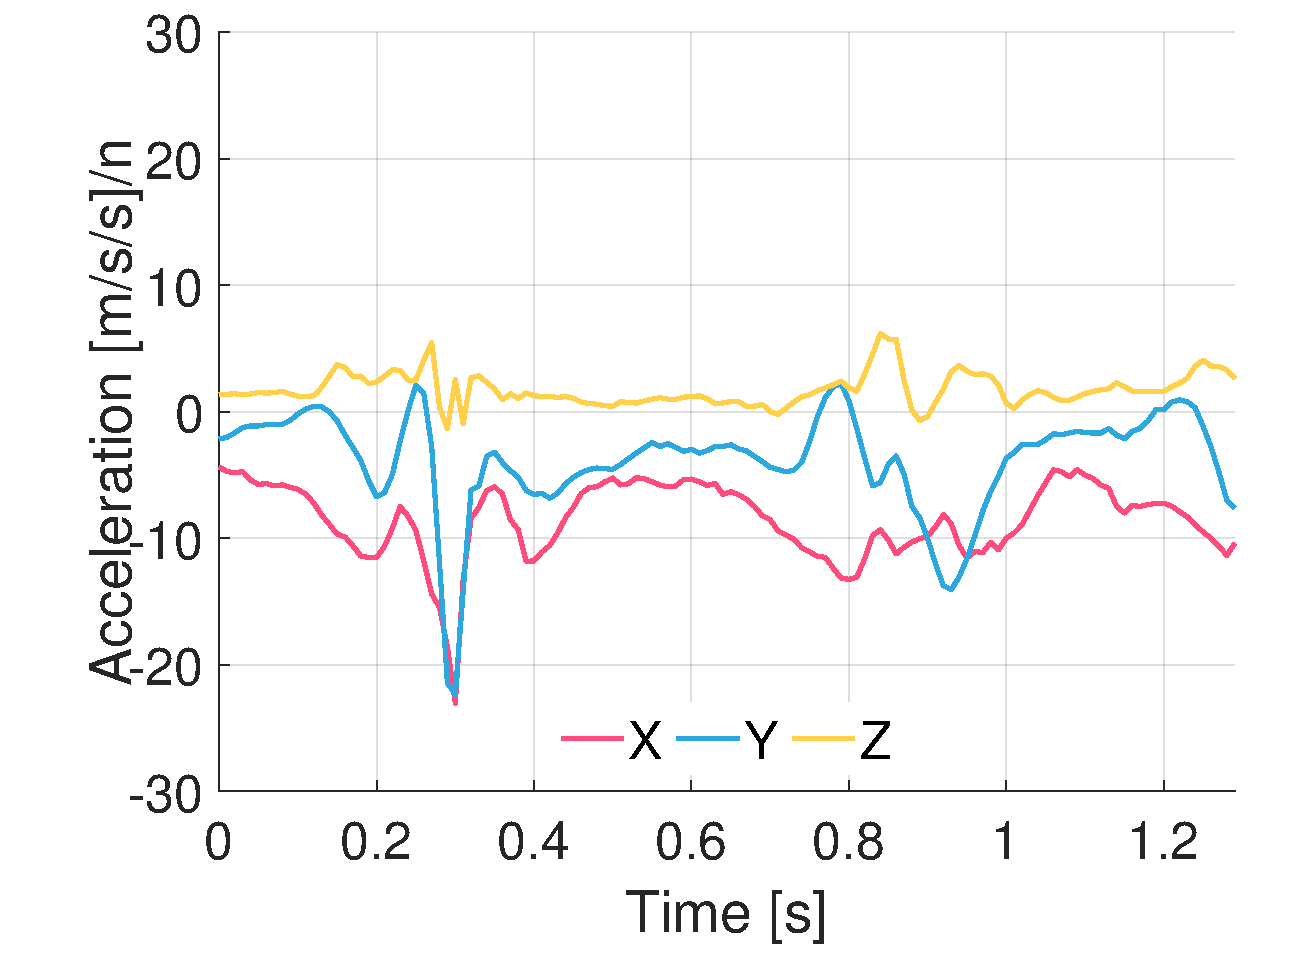
\includegraphics[width=\textwidth]{content/3-Methods/example-data/ch3_example_data_subject_01_r_hip_accel_activity_walking.pdf}
         \caption{Walking}
    \end{subfigure}
    \begin{subfigure}[b]{0.49\textwidth}
         \centering
         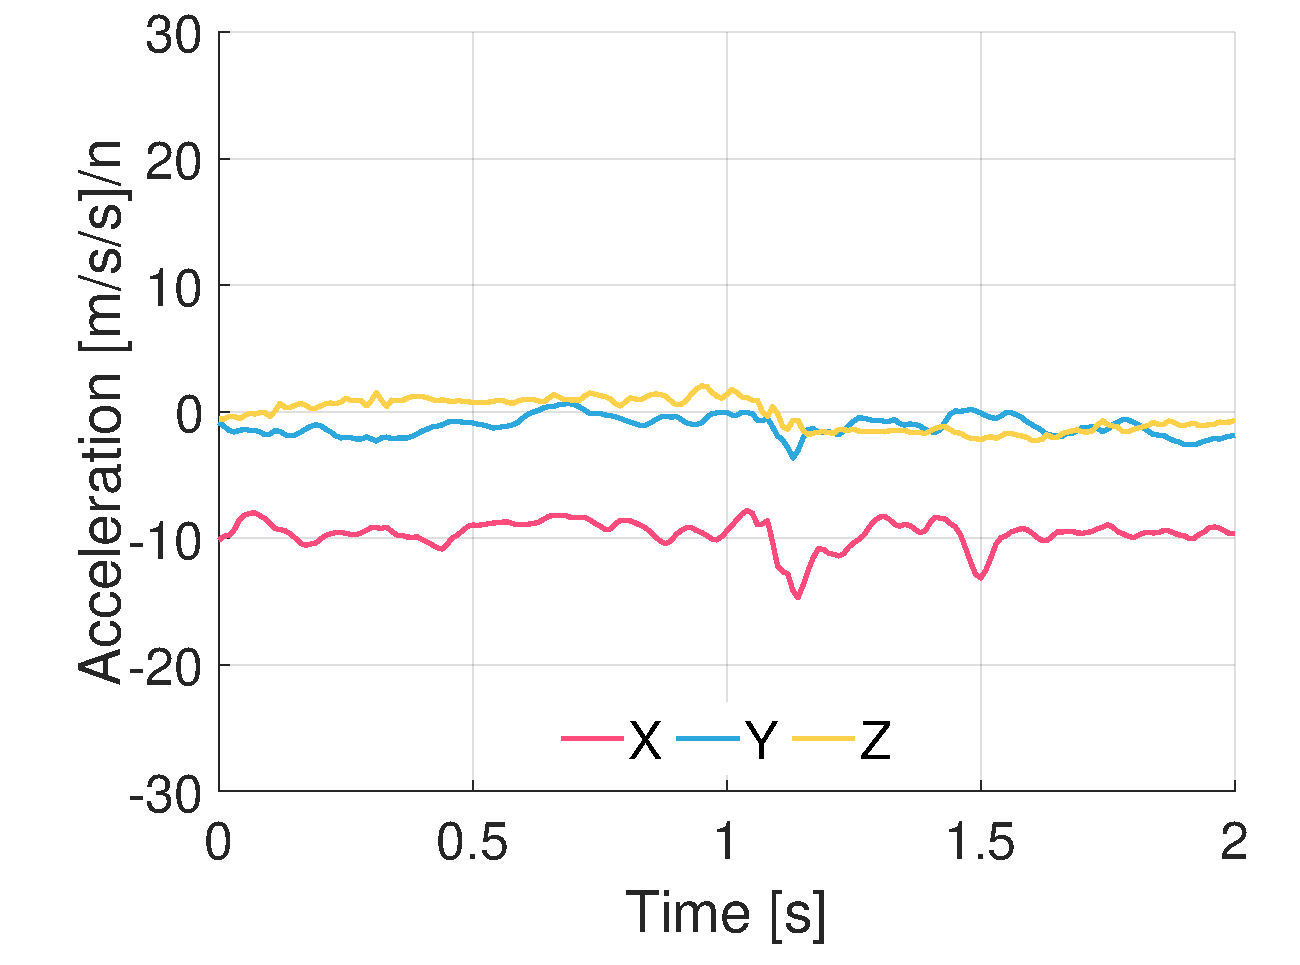
\includegraphics[width=\textwidth]{content/3-Methods/example-data/ch3_example_data_subject_01_r_hip_accel_activity_stop.pdf}
         \caption{Stopped}
    \end{subfigure}
    
    \begin{subfigure}[b]{0.49\textwidth}
         \centering
         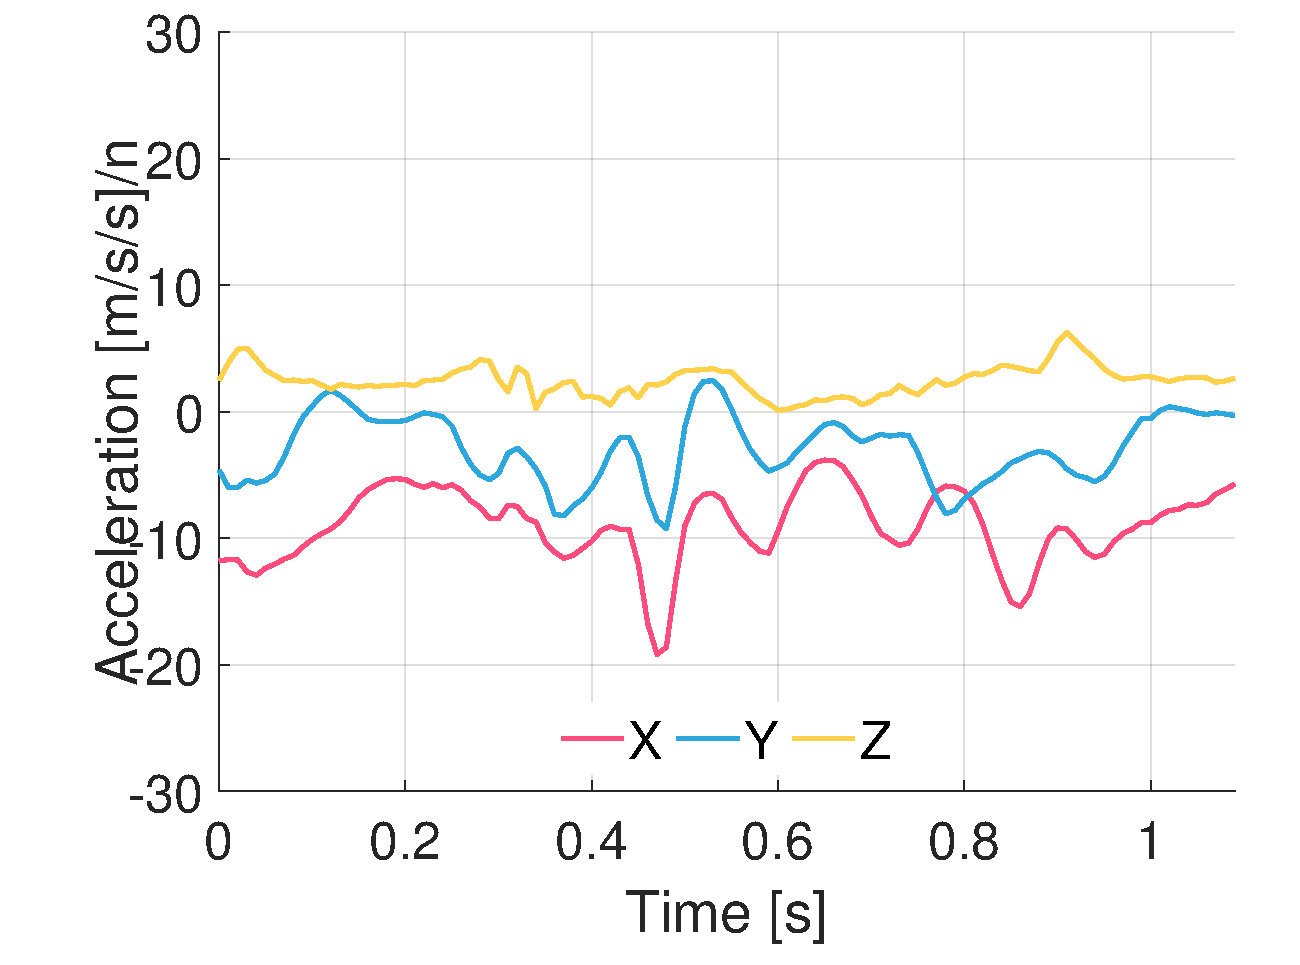
\includegraphics[width=\textwidth]{content/3-Methods/example-data/ch3_example_data_subject_01_r_hip_accel_activity_stair_down.pdf}
         \caption{Stair Ascent}
    \end{subfigure}
    \begin{subfigure}[b]{0.49\textwidth}
         \centering
         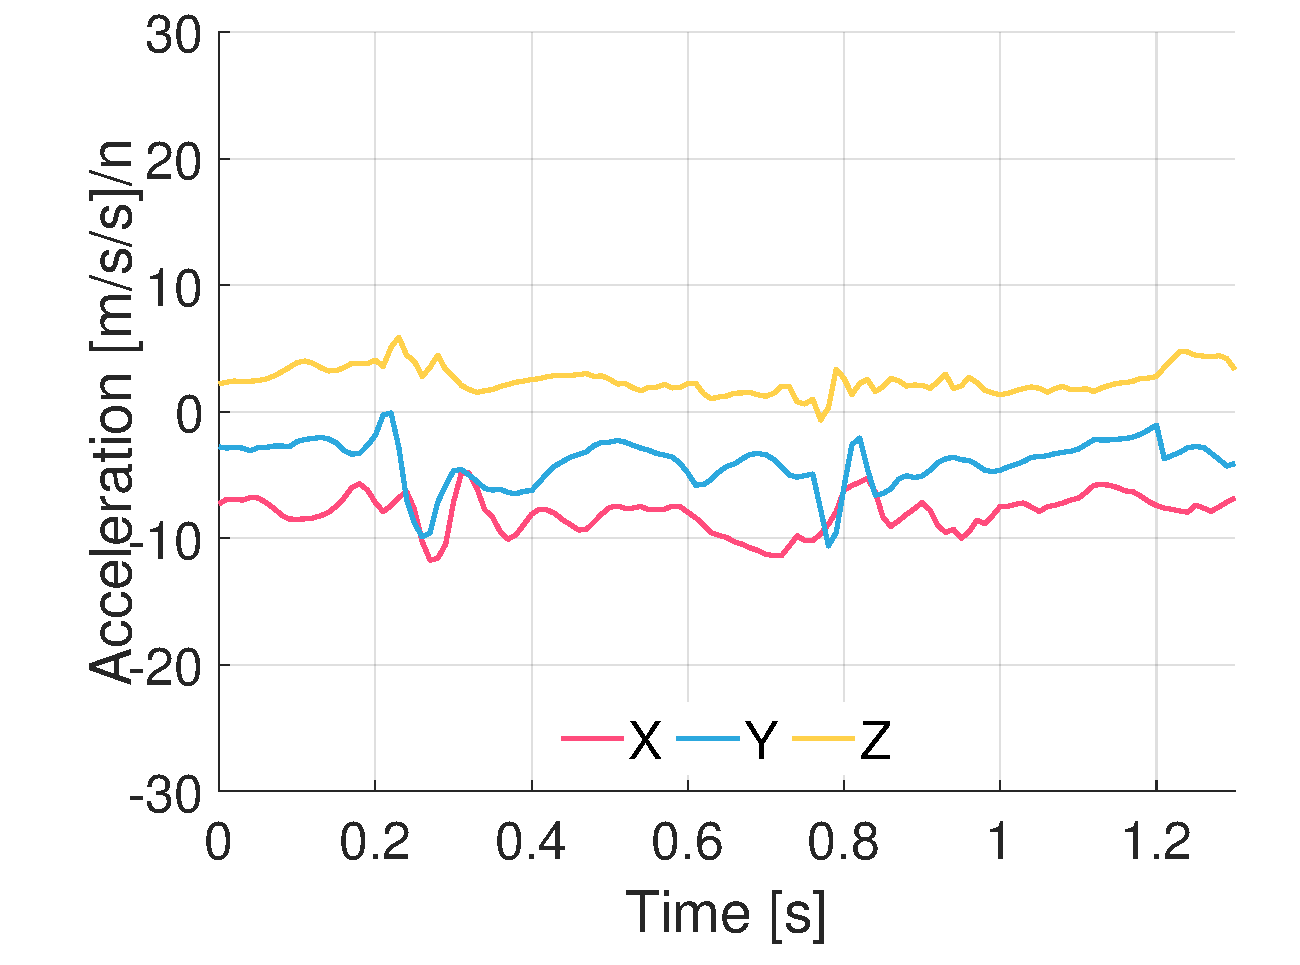
\includegraphics[width=\textwidth]{content/3-Methods/example-data/ch3_example_data_subject_01_r_hip_accel_activity_stair_up.pdf}
         \caption{Stair Descent}
    \end{subfigure}
    
    \begin{subfigure}[b]{0.49\textwidth}
         \centering
         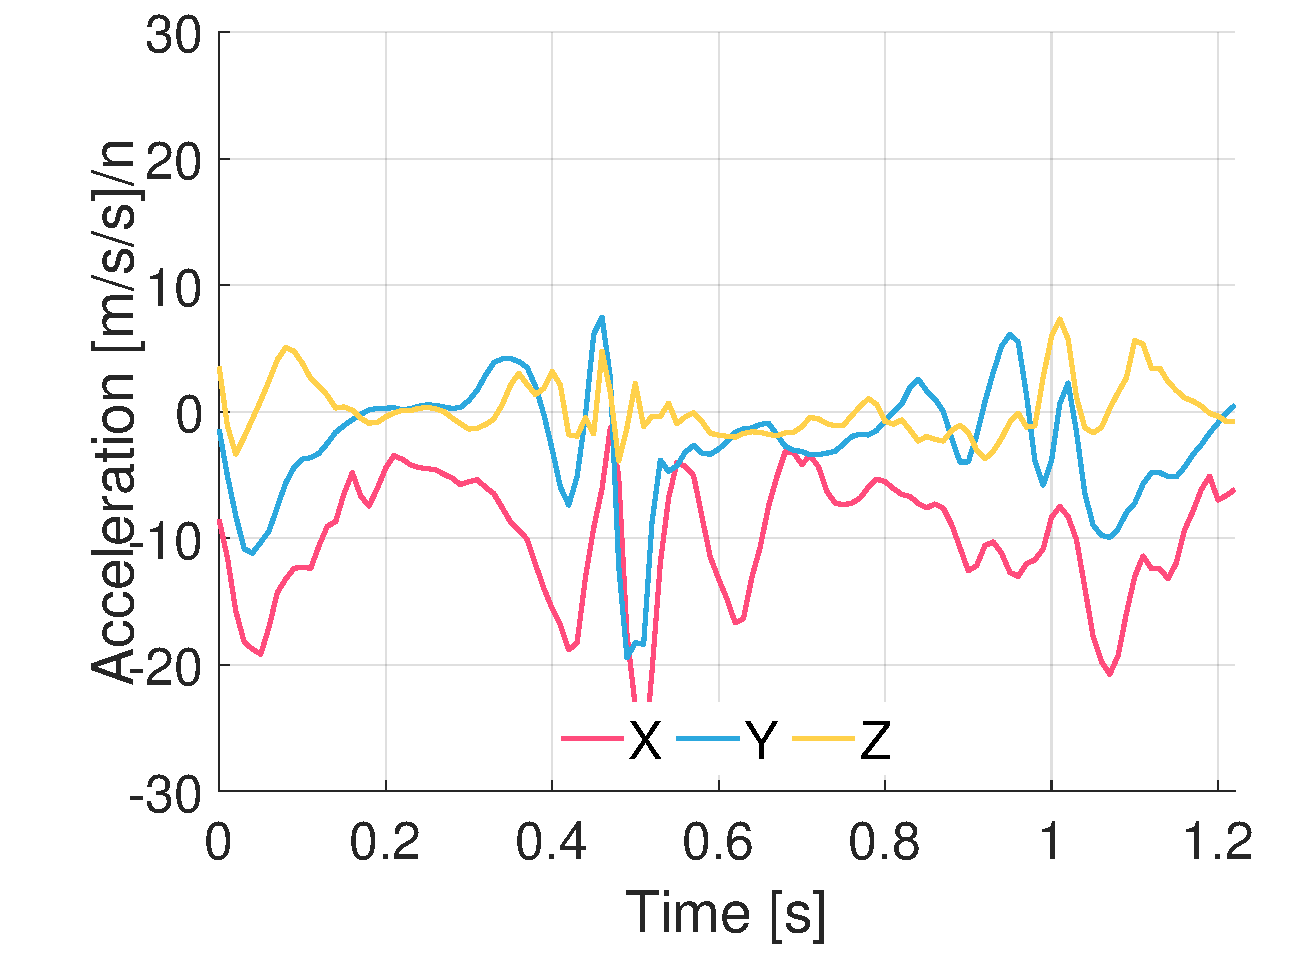
\includegraphics[width=\textwidth]{content/3-Methods/example-data/ch3_example_data_subject_01_r_hip_accel_activity_ramp_up.pdf}
         \caption{Ramp Ascent}
    \end{subfigure}
    \begin{subfigure}[b]{0.49\textwidth}
         \centering
         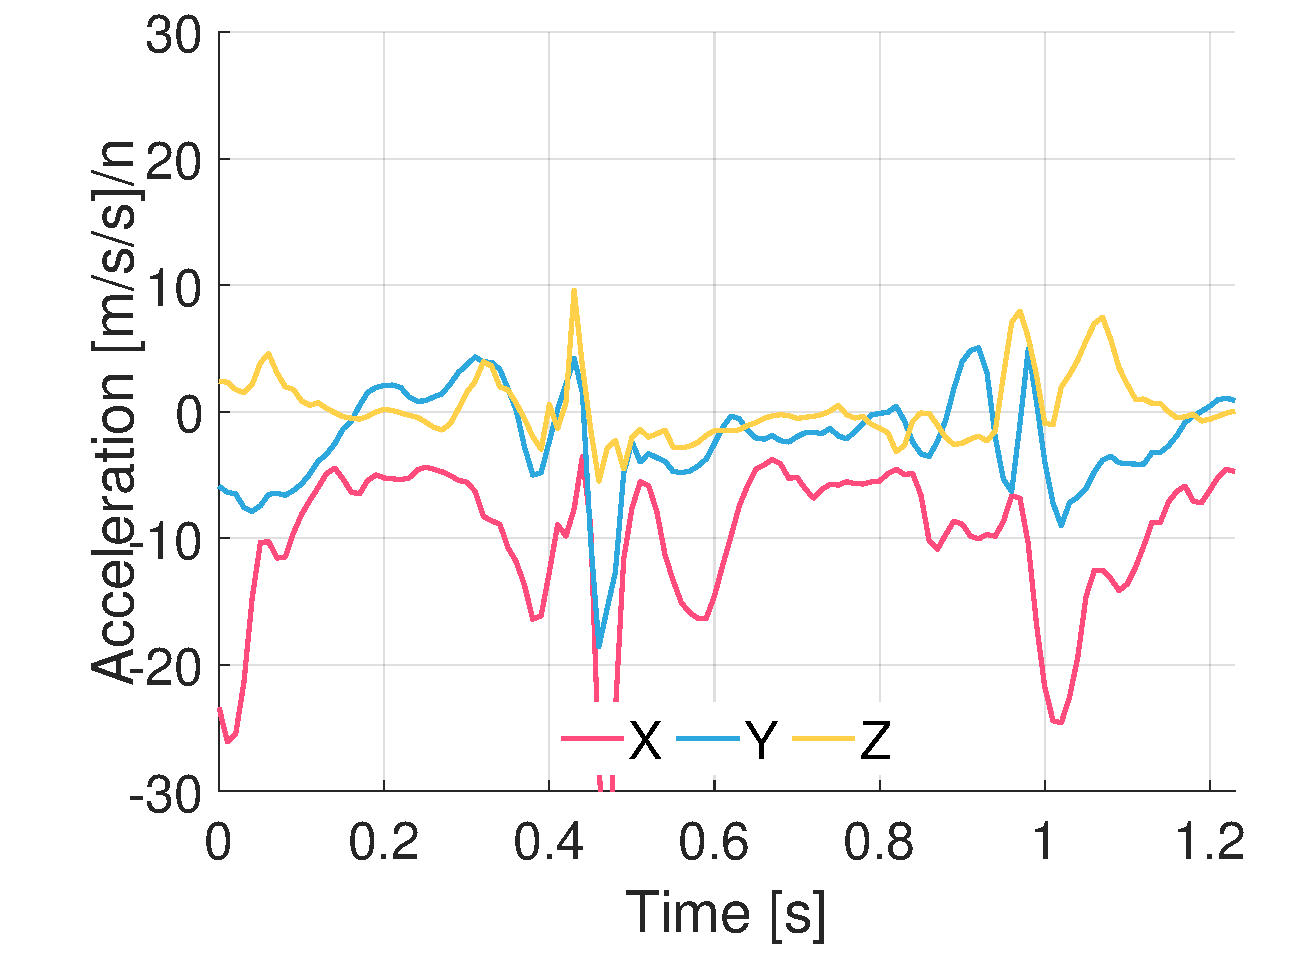
\includegraphics[width=\textwidth]{content/3-Methods/example-data/ch3_example_data_subject_01_r_hip_accel_activity_ramp_down.pdf}
         \caption{Ramp Descent}
    \end{subfigure}
    \caption[Example right hip accelerometer data]{Example data for the right hip accelerometer. The $x$ represent recording time in seconds. The y axis show the measured acceleration in m/s/s. The red lines represents the $x$ axis of the sensor, the blue solid lines the $y$ axis and the yellow lines the $z$ axis.}
    \label{fig:example-right-hip-accel-sensor-data}
\end{figure}

% Right hip gyro
\begin{figure}[p]
\centering
    \begin{subfigure}[b]{0.49\textwidth}
         \centering
         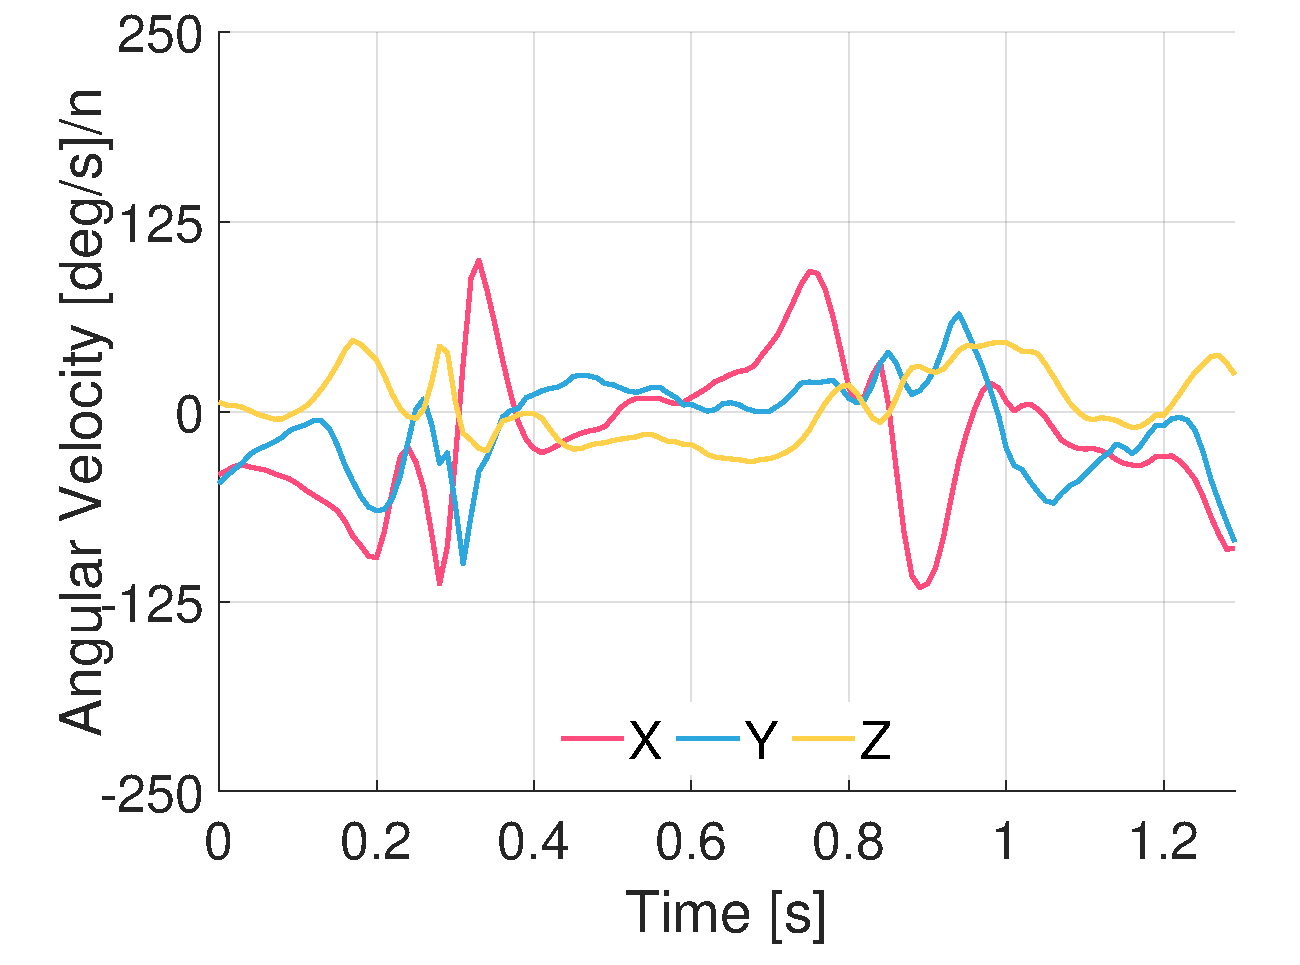
\includegraphics[width=\textwidth]{content/3-Methods/example-data/ch3_example_data_subject_01_r_hip_gyro_activity_walking.pdf}
         \caption{Walking}
    \end{subfigure}
    \begin{subfigure}[b]{0.49\textwidth}
         \centering
         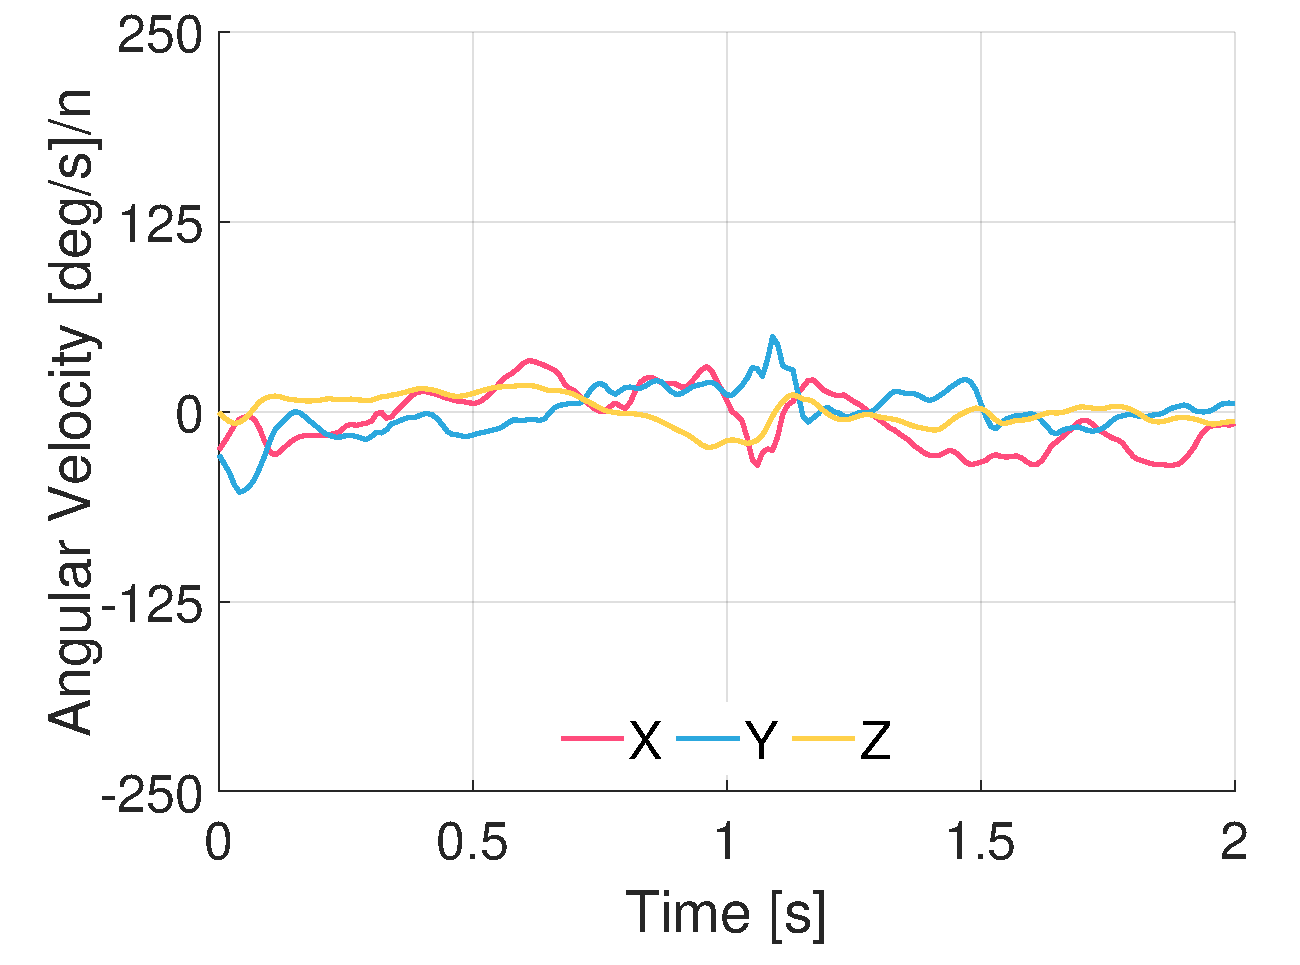
\includegraphics[width=\textwidth]{content/3-Methods/example-data/ch3_example_data_subject_01_r_hip_gyro_activity_stop.pdf}
         \caption{Stopped}
    \end{subfigure}
    
    \begin{subfigure}[b]{0.49\textwidth}
         \centering
         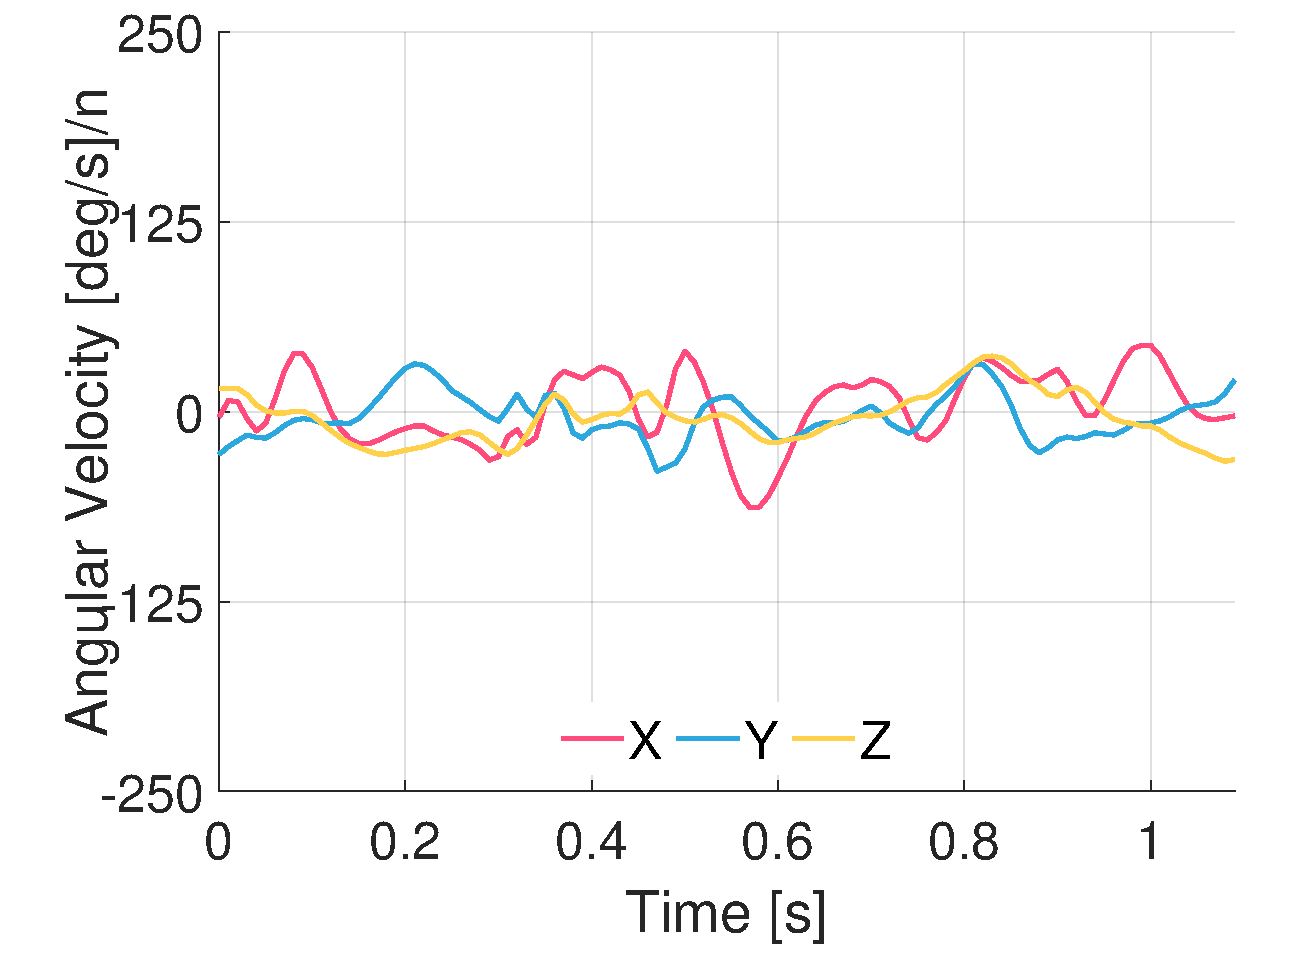
\includegraphics[width=\textwidth]{content/3-Methods/example-data/ch3_example_data_subject_01_r_hip_gyro_activity_stair_down.pdf}
         \caption{Stair Ascent}
    \end{subfigure}
    \begin{subfigure}[b]{0.49\textwidth}
         \centering
         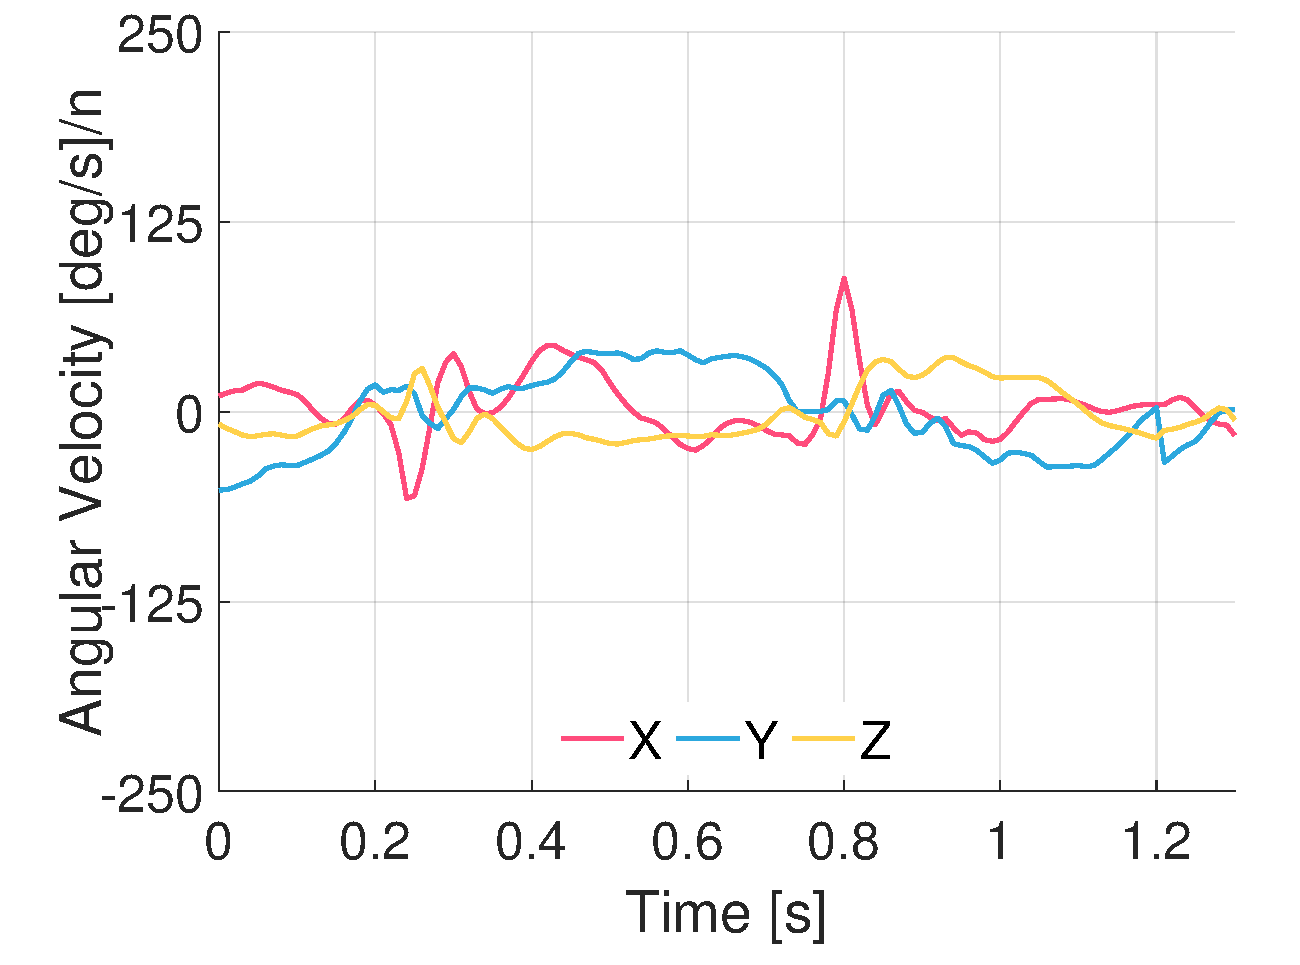
\includegraphics[width=\textwidth]{content/3-Methods/example-data/ch3_example_data_subject_01_r_hip_gyro_activity_stair_up.pdf}
         \caption{Stair Descent}
    \end{subfigure}
    
    \begin{subfigure}[b]{0.49\textwidth}
         \centering
         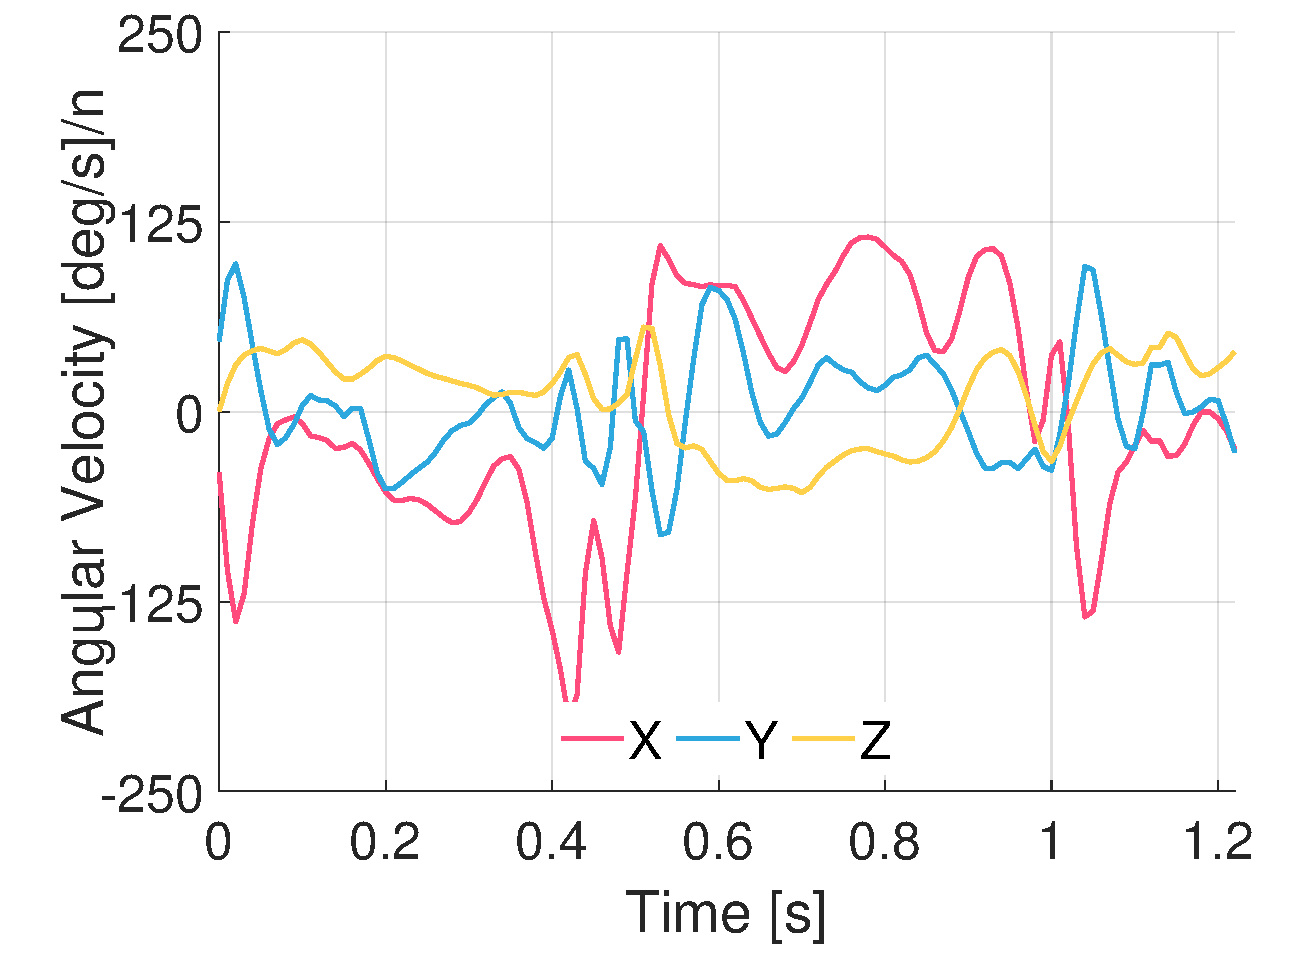
\includegraphics[width=\textwidth]{content/3-Methods/example-data/ch3_example_data_subject_01_r_hip_gyro_activity_ramp_up.pdf}
         \caption{Ramp Ascent}
    \end{subfigure}
    \begin{subfigure}[b]{0.49\textwidth}
         \centering
         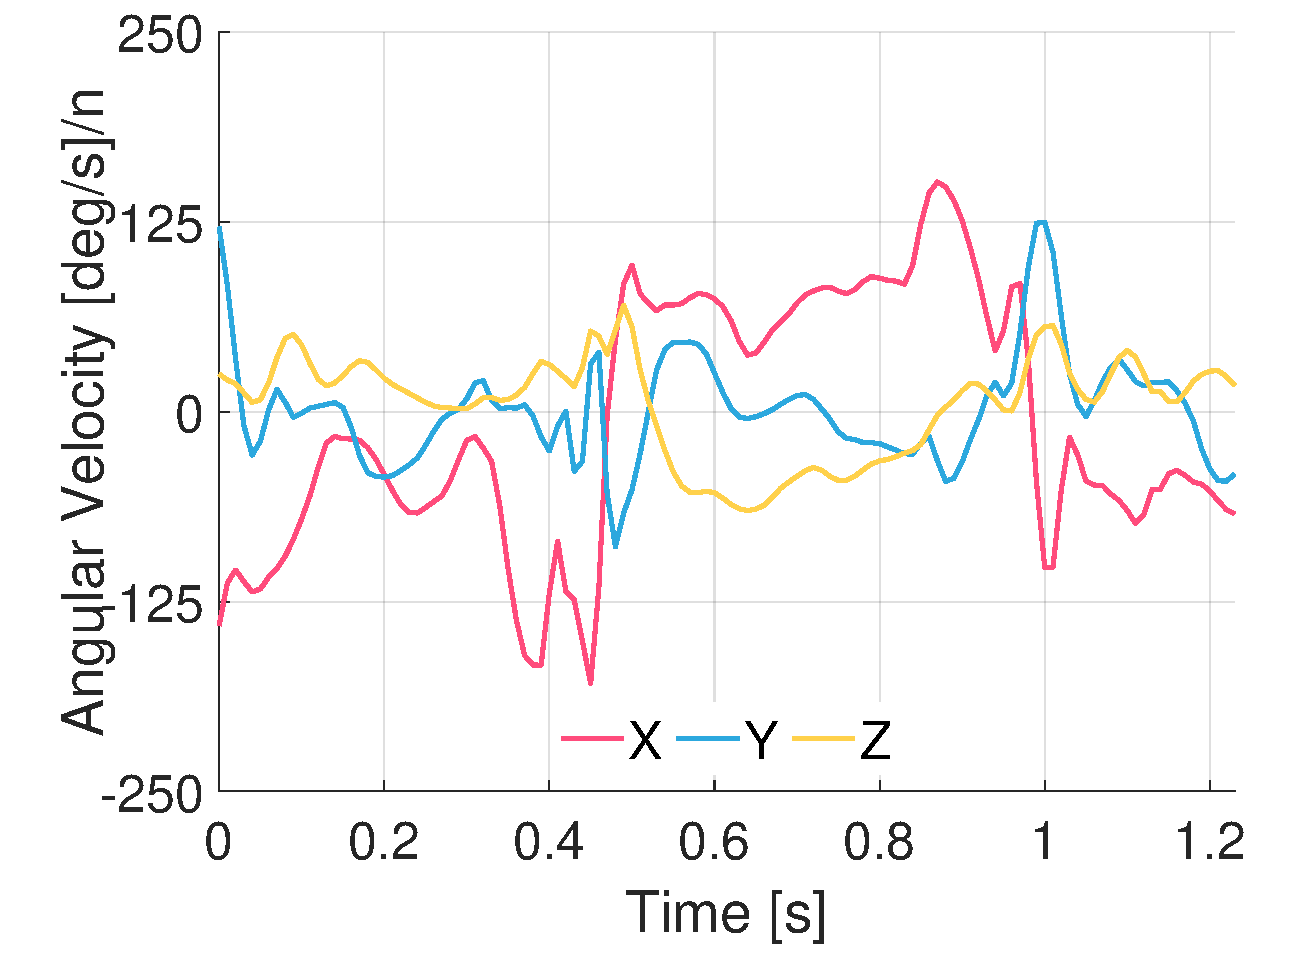
\includegraphics[width=\textwidth]{content/3-Methods/example-data/ch3_example_data_subject_01_r_hip_gyro_activity_ramp_down.pdf}
         \caption{Ramp Descent}
    \end{subfigure}
    \caption[Example right hip gyroscope data]{Example data for the right hip gyroscope. The $x$ represent recording time in seconds. The y axis show the measured angular velocity in deg/s. The red lines represents the $x$ axis of the sensor, the blue solid lines the $y$ axis and the yellow lines the $z$ axis.}
    \label{fig:example-right-hip-gyro-sensor-data}
\end{figure}

%---------------------- LEFT Chest ------------------------
% Chest accelerometer
\begin{figure}[p]
\centering
    \begin{subfigure}[b]{0.49\textwidth}
         \centering
         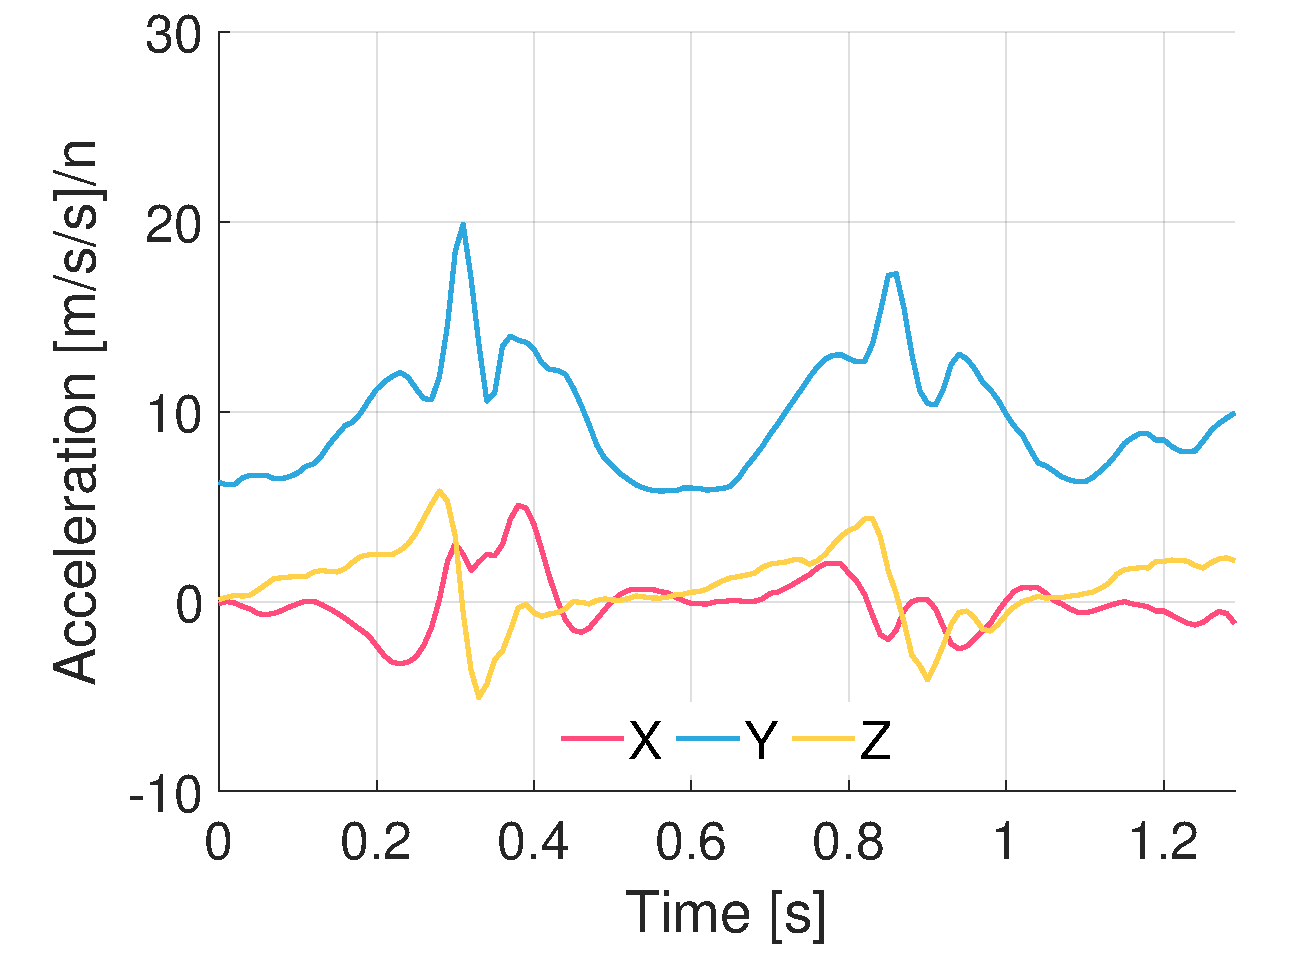
\includegraphics[width=\textwidth]{content/3-Methods/example-data/ch3_example_data_subject_01_chest_accel_activity_walking.pdf}
         \caption{Walking}
    \end{subfigure}
    \begin{subfigure}[b]{0.49\textwidth}
         \centering
         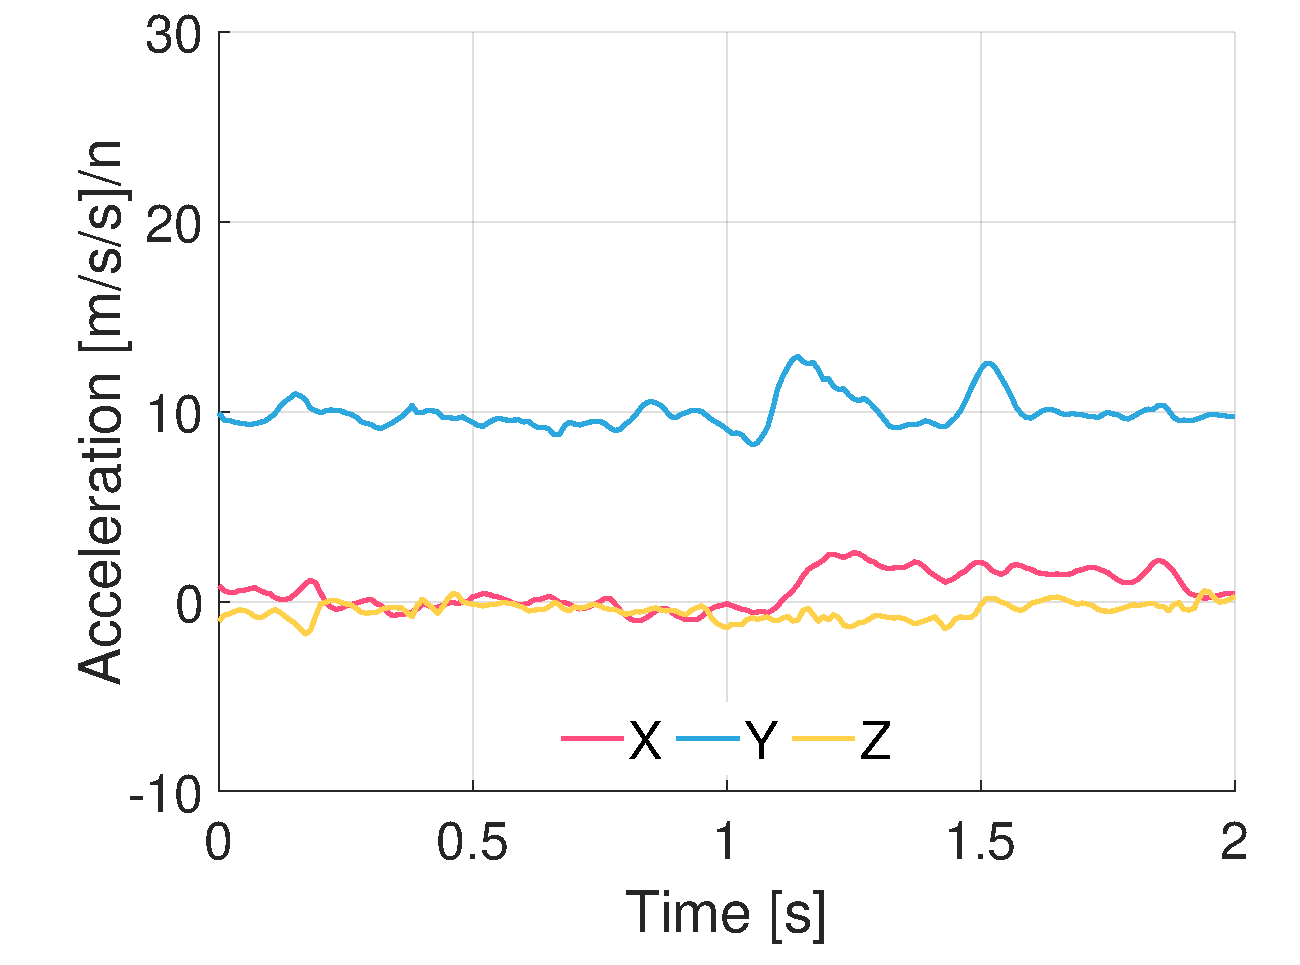
\includegraphics[width=\textwidth]{content/3-Methods/example-data/ch3_example_data_subject_01_chest_accel_activity_stop.pdf}
         \caption{Stopped}
    \end{subfigure}
    
    \begin{subfigure}[b]{0.49\textwidth}
         \centering
         \includegraphics[width=\textwidth]{content/3-Methods/example-data/ch3_example_data_subject_01_chest_accel_activity_stair_down.pdf}
         \caption{Stair Ascent}
    \end{subfigure}
    \begin{subfigure}[b]{0.49\textwidth}
         \centering
         \includegraphics[width=\textwidth]{content/3-Methods/example-data/ch3_example_data_subject_01_chest_accel_activity_stair_up.pdf}
         \caption{Stair Descent}
    \end{subfigure}
    
    \begin{subfigure}[b]{0.49\textwidth}
         \centering
         \includegraphics[width=\textwidth]{content/3-Methods/example-data/ch3_example_data_subject_01_chest_accel_activity_ramp_up.pdf}
         \caption{Ramp Ascent}
    \end{subfigure}
    \begin{subfigure}[b]{0.49\textwidth}
         \centering
         \includegraphics[width=\textwidth]{content/3-Methods/example-data/ch3_example_data_subject_01_chest_accel_activity_ramp_down.pdf}
         \caption{Ramp Descent}
    \end{subfigure}
    \caption[Example chest accelerometer data]{Example data for the chest accelerometer. The $x$ represent recording time in seconds. The y axis show the measured acceleration in m/s/s. The red lines represents the $x$ axis of the sensor, the blue solid lines the $y$ axis and the yellow lines the $z$ axis.}
    \label{fig:example-chest-accel-sensor-data}
\end{figure}

% Chest gyro
\begin{figure}[p]
\centering
    \begin{subfigure}[b]{0.49\textwidth}
         \centering
         \includegraphics[width=\textwidth]{content/3-Methods/example-data/ch3_example_data_subject_01_chest_gyro_activity_walking.pdf}
         \caption{Walking}
    \end{subfigure}
    \begin{subfigure}[b]{0.49\textwidth}
         \centering
         \includegraphics[width=\textwidth]{content/3-Methods/example-data/ch3_example_data_subject_01_chest_gyro_activity_stop.pdf}
         \caption{Stopped}
    \end{subfigure}
    
    \begin{subfigure}[b]{0.49\textwidth}
         \centering
         \includegraphics[width=\textwidth]{content/3-Methods/example-data/ch3_example_data_subject_01_chest_gyro_activity_stair_down.pdf}
         \caption{Stair Ascent}
    \end{subfigure}
    \begin{subfigure}[b]{0.49\textwidth}
         \centering
         \includegraphics[width=\textwidth]{content/3-Methods/example-data/ch3_example_data_subject_01_chest_gyro_activity_stair_up.pdf}
         \caption{Stair Descent}
    \end{subfigure}
    
    \begin{subfigure}[b]{0.49\textwidth}
         \centering
         \includegraphics[width=\textwidth]{content/3-Methods/example-data/ch3_example_data_subject_01_chest_gyro_activity_ramp_up.pdf}
         \caption{Ramp Ascent}
    \end{subfigure}
    \begin{subfigure}[b]{0.49\textwidth}
         \centering
         \includegraphics[width=\textwidth]{content/3-Methods/example-data/ch3_example_data_subject_01_chest_gyro_activity_ramp_down.pdf}
         \caption{Ramp Descent}
    \end{subfigure}
    \caption[Example chest gyroscope data]{Example data for the chest gyroscope. The $x$ represent recording time in seconds. The y axis show the measured angular velocity in deg/s. The red lines represents the $x$ axis of the sensor, the blue solid lines the $y$ axis and the yellow lines the $z$ axis.}
    \label{fig:example-chest-gyro-sensor-data}
\end{figure}
